\documentclass[lang=cn,10pt]{elegantbook}
\usepackage{physics}
\usepackage{hyperref}
\title{Somethings Strange}

\author{\textit{Astolfo}}

\extrainfo{Too young too simple, sometimes naive.}

\setcounter{tocdepth}{3}

\cover{cover.png}

% 本文档命令
\usepackage{array}
\newcommand{\ccr}[1]{\makecell{{\color{#1}\rule{1cm}{1cm}}}}

% 修改标题页的橙色带
% \definecolor{customcolor}{RGB}{32,178,170}
% \colorlet{coverlinecolor}{customcolor}

\begin{document}

\maketitle
\frontmatter


\mainmatter
\tableofcontents
\chapter{量子化学初步}
\section{量子力学基本假设}
\subsection{态叠加原理与完备性假设}
我们用$\ket{\cdot}$表示一个量子态。
\begin{theorem}[态叠加原理]
如果一个系统在测量中被发现有概率处于一系列态$\{\ket{\phi_{\alpha}}\}$,除此之外没有别的可能,那么这个系统的叠加态被定义为:
\[\ket{\psi}=\sum_{\alpha}c_{\alpha}\ket{\phi_{\alpha}}, \quad \text{满足归一化:} \sum_{\alpha}|c_{\alpha}|^2=1, \quad c_{\alpha}\in\mathbb{C}\]
\end{theorem}

需要说明的是这里我们认为所有的态$\{\ket{\phi_{\alpha}}\}$线性无关。因为我们可以考虑对线性相关的某个态再利用态叠加原理,使之由一系列线性无关的态组合而来,最终把所有线性相关的态都如上处理后,我们会发现所有的叠加态都可以被线性无关的态线性组合表示。这些线性无关的态构成了一组系统状态空间的一组基底。同时由于观测后系统只能处于唯一的某一个态上,但是\textcolor{blue}{\textbf{基底之间相互独立并不意味着基底之间相互正交}},但是非正交的基底可以通过标准正交化变换成标准正交基,我们没有必要在入门量子力学的时候你们早就处理折磨复杂的体系(疑似有点抖M)。于是我们直接默认系统中的所有态构成标准正交基,即$\ket{\alpha}^{\dagger}\ket{\alpha‘}=\delta_{\alpha\alpha'}$。

从上述的描述中我们不难发现,态叠加原理实质上是假设\textcolor{blue}{\textbf{量子态空间是线性的}}。同时在定义中我们引入了“除此之外别无可能”的表述,这表明该这一系列量子态张成的空间$\text{Span}\{\ket{\phi_{\alpha}}\}$是完备的。我们一般称测量中能观测到的态为纯态(对应混合态),两者统称为波函数。

我们可以做出如下论断,态叠加原理假设了量子力学中\textcolor{blue}{\textbf{量子态空间是$\mathbb{C}$上的一个完备的线性空间}}。上述的论述中我们提到了所有可及的态都是观测得来的,这就有了完备性假设的一个等价表述:\textcolor{blue}{\textbf{算符的本征态张成的空间是完备的}}。虽然目前我们还没定义什么是算符反正我先把这句话放这了。Ciallo$\sim$($\angle$$\cdot$$\omega$< )$\frown$$\star$


在这样的一个完备的线性空间上我们可以定义内积:
\begin{definition}[内积]
设 $V$ 是数域 $\mathbb{F}$(通常为实数域 $\mathbb{R}$ 或复数域 $\mathbb{C}$)上的线性空间。若映射 $\langle \cdot, \cdot \rangle: V \times V \to \mathbb{F}$ 满足以下性质:
\begin{enumerate}
    \item \textbf{正定性}:对任意 $\mathbf{x} \in V$,有 $\langle \mathbf{x}, \mathbf{x} \rangle \geq 0$,且 $\langle \mathbf{x}, \mathbf{x} \rangle = 0$ 当且仅当 $\mathbf{x} = \mathbf{0}$;
    \item \textbf{共轭对称性}:对任意 $\mathbf{x}, \mathbf{y} \in V$,有 $\langle \mathbf{x}, \mathbf{y} \rangle = \overline{\langle \mathbf{y}, \mathbf{x} \rangle}$;
    \item \textbf{线性性}:对任意 $\mathbf{x}, \mathbf{y}, \mathbf{z} \in V$ 和任意 $a, b \in \mathbb{F}$,有
    \[
    \langle a\mathbf{x} + b\mathbf{y}, \mathbf{z} \rangle = a^*\langle \mathbf{x}, \mathbf{z} \rangle + b^*\langle \mathbf{y}, \mathbf{z} \rangle, \quad \langle \mathbf{z}, a\mathbf{x} + b\mathbf{y} \rangle = z\langle \mathbf{z}, \mathbf{x} \rangle + b\langle \mathbf{z}, \mathbf{y} \rangle.
    \]
\end{enumerate}
则称 $\langle \cdot, \cdot \rangle$ 为 $V$ 上的一个内积。
\end{definition}
装备了内积的线性空间称为内积空间。内积诱导的范数定义为$\|\mathbf{x}\| = \sqrt{\langle \mathbf{x}, \mathbf{x} \rangle}$。若内积空间关于诱导范数完备,则称为希尔伯特空间。权且当上述定义的态空间是完备的希尔伯特空间,证明或者证伪留着以后再说。

因此我们定义态空间的内积:
\[\forall f,g \in \text{Span}\{\ket{\phi_{\alpha}}\}, \quad \langle f,g \rangle=\ket{f}^{\dagger}\ket{g}=\sum_{\alpha\alpha'}c_{f\alpha}^*c_{g\alpha'}\ket{\phi_{\alpha}}^{\dagger}\ket{\phi_{\alpha}}=\sum_{\alpha}c_{f\alpha}^*c_{g\alpha}\]

根据定义,任意一个叠加态都是归一化的:
\[\|\psi\|=\sqrt{\langle\psi,\psi\rangle}=\sqrt{\sum_{\alpha}|c_{\alpha}|^2}=1\]
\subsection{统计诠释与算符}
我们定义$\bra{\cdot}$也表示一个量子态,与$\ket{\cdot}$一一对应且满足$\bra{\cdot}=\ket{\cdot}^{\dagger}$。我们分别称$\bra{\cdot}$和$\ket{\cdot}$为左矢和右矢,从上一小节我们知道右矢张成的空间是一个完备的线性空间,同时,左矢通过共轭映射(一一映射)也会生成一个完备的线性空间(这由 Riesz 表示定理保证,每个左矢对应都对应一个右矢的共轭),也满足态叠加原理:
\[\bra{\psi}=\sum_{\alpha}\bra{\phi_{\alpha}}c_{\alpha}^*, \quad \text{满足归一化:} \sum_{\alpha}|c_{\alpha}^*|^2=1\]
同时由共轭的性质我们知道$\bra{\cdot}\ket{\cdot}=|\ket{\cdot}|^2\in\mathbb{R}\subset\mathbb{C}$。 假设右矢空间$R=\text{Span}\{\ket{\cdot}\}$,那么左矢空间$L$就是右矢空间的对偶空间,其中的元素为右矢空间的线性泛函(把右矢空间的点(态)映射到数域:$R \to \mathbb{K}=\mathbb{R}\text{ or }\mathbb{C}$):
\[\bra{f}:R \to \mathbb{K} \ , \quad \ket{g} \mapsto \bra{f}\ket{g}=\ket{\phi}^{\dagger}\ket{\psi}=\sum_{\alpha\alpha'}c_{f\alpha}^*c_{g\alpha'}\ket{\phi_{\alpha}}^{\dagger}\ket{\phi_{\alpha}}=\sum_{\alpha}c_{f\alpha}^*c_{g\alpha}\]

出了泛函这种特殊的映射,我们可以来看看更普通一点的映射,我们称呼态到态的映射为算符或者算子:
\[\hat{A}:R \to R \ , \quad \ket{\psi} \mapsto \hat{A}\ket{\psi}\]

虽然可以有各种各样奇怪的映射,但是根据上一小节的假设,态空间是一个完备的赋范线性空间,当然我们也主要关注线性算子。
\begin{definition}[线性算子]
    设$X,Y$是赋范线性空间,$T$是从$X$的线性子空间$D(T) \subset X$到$Y$的映射,若其满足
    \[\forall x,y \in X \ , \ \alpha,\beta \in \mathbb{K} \ , \ T(\alpha x+\beta y)=\alpha Tx+\beta Ty\]
\end{definition}
举个例子,我们看看算符$\hat{\bm{p}}_a=\ket{\phi_a}\bra{\phi_a}$作用到态上会发生什么:
\[\hat{\bm{p}}_a\ket{\psi}=\hat{\bm{p}}_a\left(\sum_{\alpha}c_{\alpha}\ket{\phi_{\alpha}}\right)=\sum_{\alpha}c_{\alpha}\hat{\bm{p}}_a\ket{\phi_{\alpha}}=\sum_{\alpha}c_{\alpha}\ket{\phi_a}\bra{\phi_a}\ket{\phi_{\alpha}}=c_a\ket{\phi_a}\]
这个算符提取了态$\ket{\psi}$在基底$\ket{\phi_a}$上的分量,也即是投影。因此该算符也被称为投影算符。我们观察到这个系数$c_{\alpha}$神奇的性质,归一化。同时,在上一小节中我们的论述中提到了基底是系统所有可能的态,那自然而然的我们认为会联想到$|c_{\alpha}|^2$那不就是概率嘛。于是就又了量子力学的第二个基本假设:

\begin{theorem}[统计诠释]
系统处于量子态$\ket{\phi_{\alpha}}$上的概率$w_{\alpha}$正比于(归一化后取等于)混合态$\ket{\psi}$中的系数平方$|c_{\alpha}|^2$:
\[w_{\alpha}\propto|c_{\alpha}|^2=|\bra{\phi_{\alpha}}\ket{\psi}|^2\]
\end{theorem}

这里说的概率是系统处于在量子态$\ket{\phi_{\alpha}}$的概率,而非在量子态$\ket{\psi}$上具有$\ket{\phi_{\alpha}}$的概率。这个差异的重点在于统计诠释说的是测量的结果$|\bra{\phi_{\alpha}}\ket{\psi}|^2$是怎样的,而非量子态$\ket{\psi}$是怎样的。\textbf{波函数不是描述体系本身具有的性质,不是物理量,而是描述对它测量有何结果的信息,是数学量}。

在量子力学的测量理论中,测量是整个量子力学在物理上的核心,测量所用的工具:\textcolor{blue}{\textbf{算符,是量子力学的唯一观测量}};测量的对象:量子态,是量子力学中系统的描述;测量的结果:算子的本征值;测量之间的“社交”,被\textcolor{blue}{\textbf{算符的对易关系}}所描述;测量的整个过程,被量子系统的运动方程—— Schrodinger 方程描述。可以说,测量,就是代表量子力学的基本假设,诠释着量子力学的物理。

再回到算符$\hat{O}$与纯态$\ket{\phi_{\alpha}}$上,我们说纯态是使用算符能测量到的态,也即当系统处于这个态时我们观测这个系统只会看到这个态(把算符$\hat{O}$作用到纯态$\ket{\phi_{\alpha}}$上我们只会得到纯态$\ket{\phi_{\alpha}}$本身)也即\textbf{纯态就是算符的本征态}。这也是经典物理熟悉的情况,可以认为经典世界是量子世界的本征值。再以投影算符$\hat{P}_a=\ket{\phi_a}\bra{\phi_a}$为例:
\[\hat{P}_a\ket{\phi_a}=\ket{\phi_a}\bra{\phi_a}\ket{\phi_a}=\ket{\phi_a}\]

\section{表象理论}
在上一节的基本假设中我们构建了一个由算符$\hat{A}$的正交归一的本征态空间$\{\ket{\phi_{\alpha}}\}$,并引出了其对偶空间$\{\bra{\phi_{\alpha}}\}$。而表象理论的核心目的就是如何在已知的态空间表示未知的态。现在终于不用再引入什么假设可以安心搞点数学了(喜

再次重申算符$\hat{A}$的本征态空间$\{\ket{\phi_{\alpha}}\}$基底正交归一:
\[\hat{A}\ket{\phi_{\alpha}}=\phi_{\alpha}\ket{\phi_{\alpha}}, \quad \bra{\phi_{\alpha}}\ket{\phi_{\alpha'}}=\delta_{\alpha\alpha'}\]
因此我们有:
\[\bra{\phi_{\alpha'}}\hat{A}\ket{\phi_{\alpha}}=\bra{\phi_{\alpha'}}\left(\phi_{\alpha}\ket{\phi_{\alpha}}\right)=\phi_{\alpha}\bra{\phi_{\alpha'}}\ket{\phi_{\alpha}}=\delta_{\alpha\alpha'}\phi_{\alpha}\]
不要对这个三明治感到惊讶($^{\circ}$o$^{\circ}$;;,似乎我们还没定义这是什么,这没什么(杰哥音),算符作用到态上后拿到的是另外一个态,你只是在拿一个左矢作用到一个新的右矢上算个内积而已。先别管这个,上面我们在做的是计算了算符$\hat{A}$在基底$\{\ket{\phi_{\alpha}}\}$下的“矩阵元”。你可能觉得这似乎就是矩阵元,但不是的,我没说这基底是有限的啊,甚至都没说这基底是可数的啊,那矩阵又何从谈起呢?话说回来,算符就可以写成如下形式:
\[\hat{A}=\sum_{\alpha}\ket{\phi_{\alpha}}\phi_{\alpha}\bra{\phi_{\alpha}}\]

再引入一个数学概念,我们之前定义了右矢空间的对偶空间,左矢空间,同时也知道,算符作用在右矢态上得到的是一个新的右矢态,两者结合一下就有:
\begin{definition}[伴随算符]
$\hat{A}^{\dagger}$是定义在右矢空间$R=\{\ket{\cdot}\}$的对偶空间$L=\{\bra{\cdot}\}$上的算符,存在唯一的定义在$R$上的算符$\hat{A}$满足
\[\forall \, \ket{\psi} \in R, \quad \bra{\psi}\hat{A}^{\dagger}=\hat{A}\ket{\psi}\]
如果一个算子的伴随算子是自身则称这类算子为自拌算符或者厄米算符。
\end{definition}

伴随算符具有以下性质(继续无脑假定态空间具有自反性,哎哎傻逼物理,严谨性这块烂完了):
\[\bra{\phi}\hat{A}^{\dagger}\ket{\psi}=\left(\bra{\psi}\hat{A}\ket{\phi}\right)^{\dagger}\]

\paragraph*{自拌算子的本征值为实数:}
\[A_{\psi}=\bra{\psi}\hat{A}\ket{\psi}=\bra{\psi}\hat{A}^{\dagger}\ket{\psi}=\left(\bra{\psi}\hat{A}\ket{\psi}\right)^{\dagger}=A_{\psi}^* \quad \Rightarrow \quad A_{\psi}\in\mathbb{R}\]

\paragraph*{自拌算子对应不同本征值的本征态正交:}
\[A_{\psi}\bra{\phi}\ket{\psi}=\bra{\phi}\hat{A}\ket{\psi}=\left(\bra{\psi}\hat{A}^{\dagger}\ket{\phi}\right)^{\dagger}=\left(\bra{\psi}\hat{A}\ket{\phi}\right)^{\dagger}=A_{\phi}^*\bra{\psi}\ket{\phi}^{\dagger}=A_{\phi}\bra{\phi}\ket{\psi} \quad \Rightarrow \quad \bra{\phi}\ket{\psi}=0\]

为什么要强调厄米算符这个概念,很简单,现实中我们能观测到的物理量都是实数的,我们自然而然会认为对应物理量的算符都是厄米的,这也算量子力学的一个假设:\textcolor{blue}{\textbf{观测物理量都对应一个厄米算符}}。

我们考虑一个特殊一点的算符——把对应所有基底的投影算符加起来——并计算这个新算符的矩阵元:
\[\sum_{\alpha}\ket{\phi_{\alpha}}\bra{\phi_{\alpha}} \quad \Rightarrow \quad \bra{\phi_{\alpha'}}\left(\sum_{\alpha}\ket{\phi_{\alpha}}\bra{\phi_{\alpha}}\right)\ket{\phi_{\alpha''}}=\sum_{\alpha}\bra{\phi_{\alpha'}}\ket{\phi_{\alpha}}\bra{\phi_{\alpha}}\ket{\phi_{\alpha''}}=\sum_{\alpha}\delta_{\alpha'\alpha}\delta_{\alpha\alpha''}=\delta_{\alpha'\alpha''}\]

于是我们得到了一个$\mathbbm{1}$:
\[\mathbbm{1}=\sum_{\alpha}\ket{\phi_{\alpha}}\bra{\phi_{\alpha}}\]

这个$\mathbbm{1}$可谓是表象理论中的关键,在合适的地方插入一个$\mathbbm{1}$可以让我们很舒服——地解决很多难算的问题。比如随便给一个态$\ket{\psi}$,我怎么寄吧知道这是什么,但是把$\mathbbm{1}$作用到态$\ket{\psi}$上:
\[\ket{\psi}=\mathbbm{1}\ket{\psi}=\sum_{\alpha}\ket{\phi_{\alpha}}\bra{\phi_{\alpha}}\ket{\psi}=\sum_{\alpha}c_{\alpha}\ket{\phi_{\alpha}}\]
我们也就得到了态$\ket{\psi}$在基底$\{\ket{\phi_{\alpha}}\}$下的表示,用一些已知的态就能表示一个不知何意味的态了。

另外一个例子,我们来看看一个重要的表象,坐标表象$\{\ket{\bm{r}}\}$,坐标表象的基底代表着空间中的位置格点,当态$\ket{\psi}$投影到该基底上时得到的是该态在其上的概率密度:
\[\bra{\bm{r}}\ket{\psi}=\psi(\bm{r})\]

坐标表象由位置算符$\hat{\bm{r}}$产生,也满足正交归一性(满足$\delta$-函数),产生的可观测量$\bm{r}$是实空间的坐标:
\[\hat{\bm{r}}\ket{\bm{r}}=\bm{r}\ket{\bm{r}}, \quad \bra{\bm{r}}\ket{\bm{r}'}=\delta_{\bm{r}\bm{r}'}=\delta(\bm{r}-\bm{r}')\]

在坐标表象下计算以下内积$\bra{\psi}\ket{\psi}$,你可能会说这不一眼盯真,鉴定为1吗?戳辣,还是上面那句话,我怎么知道这寄吧态$\ket{\psi}$是什么,没有一个表象来表示没有人能知道这寄吧态到底是什么:
\[\bra{\psi}\ket{\psi}=\bra{\psi}\mathbbm{1}\ket{\psi}=\bra{\psi}\left(\sum_{\alpha}\ket{\bm{r}_{\alpha}}\bra{\bm{r}_{\alpha}}\right)\ket{\psi}=\sum_{\alpha}\bra{\psi}\ket{\bm{r}_{\alpha}}\bra{\bm{r}_{\alpha}}\ket{\psi}=\sum_{\alpha}|\psi(\bm{r}_{\alpha})|^2\]
一通操作下来,这对吗?空间格点与实数基等势,那你嗯求和不炸了吗?那到底是哪里的问题呢?当然是$\mathbbm{1}$有问题(震怒,把这个$\mathbbm{1}$抓出来魔改:
\begin{theorem}[完备性公式]
算符$\hat{A}$的本征态空间$\{\ket{\phi_{\alpha}}\}$基底满足:
\[\mathbbm{1}=\sum_{\alpha}\ket{\phi_{\alpha}}w(\alpha)\bra{\phi_{\alpha}}\]
其中$w(\alpha)$是用来避免无穷的权重因子。
\end{theorem}

这里我们需要具体说明一下,基底数量有三种情况:有限,与自然数基等势(称之为可数)以及与实数基等势或者更多(没有其他分类,不要试图挑战连续统假设)。我们之前得到的$\mathbbm{1}$仅在有限基下良定义。因此我们需要对其进行修改,引入一个权重使其不会达到无穷,这并不违背我们给出的量子力学基本假设,因为乘上一个数字并不改\textcolor{blue}{\textbf{变态}}的性质(有点高血压的。对于离散的情况秩序要假设权重$w(\alpha)=1$即可回到上述我们推导的$\mathbbm{1}$,有时候对一些兼并的态我们也可以稍微调整一下系数,不过这都是技术细节,在现在来看这个完备性公式确实比较良定义了。

在有了正确的完备性公式后,我们再来计算内积$\bra{\psi}\ket{\psi}$:
\[\bra{\psi}\ket{\psi}=\bra{\psi}\mathbbm{1}\ket{\psi}=\bra{\psi}\left(\sum_{\alpha}\ket{\bm{r}_{\alpha}}w(\alpha)\bra{\bm{r}_{\alpha}}\right)\ket{\psi}=\sum_{\alpha}\bra{\psi}\ket{\bm{r}_{\alpha}}w(\alpha)\bra{\bm{r}_{\alpha}}\ket{\psi}=\sum_{\alpha}w(\alpha)|\psi(\bm{r}_{\alpha})|^2\]

对于坐标表象$\{\ket{\bm{r}}\}$,其权重$w(\alpha)$是每个单位空间格点的体积,即$w(\alpha)=\dd{\bm{r}_{\alpha}}=\dd{\bm{r}}$,因此
\[\bra{\psi}\ket{\psi}=\sum_{\alpha}w(\alpha)|\psi(\bm{r}_{\alpha})|^2=\int_{\mathbb{R}^n}\dd{\bm{r}}|\psi(\bm{r})|^2=1\]

空间表象中的$\mathbbm{1}$即是:
\[\mathbbm{1}=\int\dd{\bm{r}}\ket{\bm{r}}\bra{\bm{r}}\]

再来另外一个例子:
\[\psi(\bm{r})=\bra{\bm{r}}\ket{\psi}=\bra{\bm{r}}\mathbbm{1}\ket{\psi}=\int\dd{\bm{r}'}\bra{\bm{r}}\ket{\bm{r}'}\bra{\bm{r}'}\ket{\psi}=\int\dd{\bm{r}'}\delta(\bm{r}'-\bm{r})\psi(\bm{r}')\]
很好得符合了数学上的定义(舒服了

坐标表象下的正交归一性表现为$\delta$-函数,多了解一点其性质有助于身心健康以及后续的学习,比如$\delta$-函数的对称性和导数性质:
\[\delta(\bm{r}-\bm{r}')=\bra{\bm{r}}\ket{\bm{r}'}=\bra{\bm{r}'}\ket{\bm{r}}^*=\bra{\bm{r}'}\ket{\bm{r}}=\delta(\bm{r}'-\bm{r}), \quad \nabla_{\bm{r}}\delta(\bm{r}-\bm{r}')=-\nabla_{\bm{r}'}\delta(\bm{r}-\bm{r}')=-\nabla_{\bm{r}'}\delta(\bm{r}'-\bm{r})\]
声明一下,$\delta(\bm{r}-\bm{r}')$的自变量是被减的$\bm{r}$,梯度算子$\nabla$的下角标表示对哪一套坐标求导。根据以上两条性质以及分部积分,我们知道:
\[\int_{\mathbb{R}^n}\nabla_{\bm{r}}\delta(\bm{r}-\bm{r}')f(\bm{r}')\dd{\bm{r}'}=-\int_{\mathbb{R}^n}\nabla_{\bm{r'}}\delta(\bm{r}'-\bm{r})f(\bm{r}')\dd{\bm{r}'}=\int_{\mathbb{R}^n}\delta(\bm{r}'-\bm{r})\nabla_{\bm{r'}}f(\bm{r}')\dd{\bm{r}'}=\nabla_{\bm{r}}f(\bm{r}) \tag{a}\label{a}\]
即:
\[\nabla_{\bm{r}}\delta(\bm{r}-\bm{r}')=\delta(\bm{r}-\bm{r}')\nabla_{\bm{r}'}\]
我们来看一个有意思的算符,定义一个“导数”算符,它把态映射到态的导数(虽然我们既不知道态是什么也不知道态的导数是什么,权且假设态的导数也在完备的态空间中):
\[\hat{D}:R \to R, \quad \ket{\psi} \mapsto \ket{\nabla\psi} \]
由于我们不知道态是什么,我们只能知道态在某个表象空间下的投影,因此,选择坐标表象:
\[\bra{\bm{r}}\hat{D}\ket{\psi}=\bra{\bm{r}}\ket{\nabla\psi}=\nabla_{\bm{r}}\psi(\bm{r})\]
这里可能有点疑惑,详细解释一下:我们知道一个函数的导数(梯度)是什么,而函数是数域到数域到一个映射,即函数的导数这个映射是建立在坐标表象之上的,因此我们抽象构建了一个“导数”算符,使得其在坐标空间下的投影就是函数的导数。
下一步我们自然而然得会去考虑,那么“导数”算符在坐标表象下的算符表示是什么呢?为例求解该表示,我们还是先来插入一个$\mathbbm{1}$:
\[\bra{\bm{r}}\hat{D}\ket{\psi}=\int_{\mathbb{R}^n}\bra{\bm{r}}\hat{D}\ket{\bm{r}'}\bra{\bm{r}'}\ket{\psi}\dd{\bm{r}'}=\int_{\mathbb{R}^n}\bra{\bm{r}}\hat{D}\ket{\bm{r}'}\psi(\bm{r}')\dd{\bm{r}'}=\nabla_{\bm{r}}\psi(\bm{r})\]
与(\ref{a})式对比,可以发现:
\[\bra{\bm{r}}\hat{D}\ket{\bm{r}'}=\nabla_{\bm{r}}\delta(\bm{r}-\bm{r}')=\delta(\bm{r}-\bm{r}')\nabla_{\bm{r}'}\]
然后我们会发现这破算符不是厄米的而是反厄米的:
\[\bra{\bm{r}'}\hat{D}\ket{\bm{r}}=\nabla_{\bm{r}'}\delta(\bm{r}'-\bm{r})=-\nabla_{\bm{r}}\delta(\bm{r}-\bm{r}')=-\bra{\bm{r}}\hat{D}\ket{\bm{r}'}=-\bra{\bm{r}}\hat{D}\ket{\bm{r}'}^{\dagger}\neq\bra{\bm{r}}\hat{D}\ket{\bm{r}'}^{\dagger}\]

解决办法就很简单了,我们定义一个新算符$\hat{\bm{p}}=-i\hbar\hat{D}$就是厄米的了:
\[\bra{\bm{r}}\hat{\bm{p}}\ket{\bm{r}'}=-i\hbar\nabla_{\bm{r}}\delta(\bm{r}-\bm{r}')=i\hbar\nabla_{\bm{r}'}\delta(\bm{r}'-\bm{r})=(-i\hbar\nabla_{\bm{r}'}\delta(\bm{r}'-\bm{r}))^*=\bra{\bm{r}'}\hat{\bm{p}}\ket{\bm{r}}^{\dagger}\]
既然知道算符$\hat{\bm{p}}$是厄米的,那么我们可以直接给出其本征态以及本征值$\hat{\bm{p}}\ket{\bm{k}}=\bm{k}\ket{\bm{k}}, \ \bm{k}\in\mathbb{R}^n$。坐标表象下我们记$\psi_{\bm{k}}(\bm{r})=\bra{\bm{r}}\ket{\bm{k}}$:
\[\bra{\bm{r}}\hat{\bm{p}}\ket{\bm{k}}=\bm{k}\bra{\bm{r}}\ket{\bm{k}}=k\psi_{\bm{k}}(\bm{r})\]
\[\bra{\bm{r}}\hat{\bm{p}}\ket{\bm{k}}=\int_{\mathbb{R}^n}\bra{\bm{r}}\hat{\bm{p}}\ket{\bm{r}'}\bra{\bm{r}'}\ket{\bm{k}}\dd{\bm{r}'}=-i\hbar\int_{\mathbb{R}^n}\delta(\bm{r}-\bm{r}')\nabla_{\bm{r}'}\psi_{\bm{k}}(\bm{r}')\dd{\bm{r}'}=-i\hbar\nabla_{\bm{r}}\psi_{\bm{k}}(\bm{r})=\bm{k}\psi_{\bm{k}}(\bm{r})\]
利用分离变量法可以轻松求解上述微分方程:
\[\bra{\bm{r}}\ket{\bm{k}}=\psi_{\bm{k}}(\bm{r})=\frac{1}{\sqrt{2\pi}}\exp\left(\frac{i\bm{k}\cdot\bm{r}}{\hbar}\right)\]
很自然我们就能猜到算符$\hat{\bm{p}}=-i\hbar\nabla_{\bm{r}}$,恭喜你拿到了坐标表象下的动量算符以及它的本征态平面波$\ket{\bm{k}}$。而坐标算符$\hat{\bm{r}}$在坐标表象下就是一个数$\bm{r}$:
\[\left\{\begin{aligned}
\hat{\bm{r}} & \to \bm{r} \\ \hat{\bm{p}} & \to -i\hbar\nabla_{\bm{r}}
\end{aligned}\right.\]
类似的,如果你从动量表象出发,也可以拿到对应的坐标与动量算符:
\[\left\{\begin{aligned}
\hat{\bm{r}} & \to i\hbar\nabla_{\bm{p}} \\ \hat{\bm{p}} & \to \bm{p}
\end{aligned}\right.\]
本小节到这就快结束了,最后来个轻松愉快的小练习:证明一维动量算符$\hat{p}_x=-i\hbar\partial_x$是厄米算符:
\[\begin{aligned}
\bra{\phi}\hat{p}_x\ket{\psi}&=\int\int_{\mathbb{R}\times\mathbb{R}}\bra{\phi}\ket{x}\bra{x}\hat{p}_x\ket{x'}\bra{x'}\ket{\psi}\dd{x}\dd{x'}=\int\int_{\mathbb{R}\times\mathbb{R}}\phi^*(x)[-i\hbar\delta(x-x')\partial_{x'}]\psi(x')\dd{x}\dd{x'}\\
&=\int_{-\infty}^{\infty}\phi^*(x)[-i\hbar\partial_{x}]\psi(x)\dd{x}=-i\hbar\int_{-\infty}^{\infty}\phi^*(x)\dd{\psi(x)}=-i\hbar\eval{\phi^*(x)\psi(x)}_{-\infty}^{\infty}+i\hbar\int_{-\infty}^{\infty}\psi^*(x)\dd{\phi(x)}\\
&=\int_{-\infty}^{\infty}\psi^*(x)[i\hbar\partial_x]\phi(x)\dd{x}=\bra{\psi}\hat{p}_x^{\dagger}\ket{\phi}=\bra{\phi}\hat{p}_x\ket{\psi}^{\dagger}
\end{aligned}\]

\subsection{表象变换}
表象理论的一大核心内容是表象之间的变换,这也是$\mathbbm{1}$发挥作用的重要领域。表象变换也即态空间的基底变换,假设我们已知基底$\{\ket{\phi_{\alpha}}\}$,某两个态$\ket{p},\ket{q}$与算符$\hat{O}$,则内积$\bra{p}\ket{q}$与算符$\hat{O}$在基底$\{\ket{\phi_{\alpha}}\}$下的表示为:
\[\bra{p}\ket{q}=\bra{p}\mathbbm{1}\ket{q}=\sum_{\alpha}\bra{p}\ket{\phi_{\alpha}}w(\alpha)\bra{\phi_{\alpha}}\ket{q}=\sum_{\alpha}w(\alpha)c_{p\alpha}^*c_{q\alpha}\]
\[\hat{O}=\mathbbm{1}\hat{O}\mathbbm{1}=\sum_{\alpha\alpha'}\ket{\phi_{\alpha}}w(\alpha)\bra{\phi_{\alpha}}\hat{O}\ket{\phi_{\alpha'}}w(\alpha')\bra{\phi_{\alpha'}}:=\sum_{\alpha\alpha'}\ket{\phi_{\alpha}}w(\alpha)O_{\alpha\alpha'}w(\alpha')\bra{\phi_{\alpha'}}\]
这里$O_{\alpha\alpha'}$是算符在基底$\{\ket{\phi_{\alpha}}\}$下的生成元,这里给出正式名称,再叫矩阵元就不礼貌了。这里突然想到,我们既然可以给内积中间插入一个$\mathbbm{1}$算符,我们能不能插入其他算符呢?比如:
\[\bra{p}\hat{O}\ket{q}=\sum_{\alpha\alpha'}\bra{p}\ket{\phi_{\alpha}}w(\alpha)O_{\alpha\alpha'}w(\alpha')\bra{\phi_{\alpha'}}\ket{q}=\sum_{\alpha\alpha'}c_{p\alpha}^*w(\alpha)O_{\alpha\alpha'}w(\alpha')c_{q\alpha'}\]
当$\ket{q}=\ket{p}$时,有:
\[\langle\hat{O}\rangle=\bra{p}\hat{O}\ket{p}=\sum_{\alpha\alpha'}\bra{p}\ket{\phi_{\alpha}}w(\alpha)O_{\alpha\alpha'}w(\alpha')\bra{\phi_{\alpha'}}\ket{p}=\sum_{\alpha\alpha'}c_{p\alpha}^*w(\alpha)O_{\alpha\alpha'}w(\alpha')c_{p\alpha'}\]
现在我们想说明上述表达式与数学上的期望定义相容,统计诠释告诉我们系数的平方$|c_{p\alpha}|^2$正比于概率(归一化后取等)考虑把归一化条件写成概率并对期望$\langle\hat{O}\rangle$做量纲分析:
\[\sum_{\alpha}P_p(\alpha):=\sum_{\alpha}w(\alpha)c_{p\alpha}^*c_{p\alpha}=1\]
\[\langle\hat{O}\rangle=\sum_{\alpha\alpha'}c_{p\alpha}^*w(\alpha)O_{\alpha\alpha'}w(\alpha')c_{p\alpha'}\sim\sum_{\alpha}w(\alpha)O_{\alpha\alpha}P_p(\alpha)\]
这与数学上期望的定义一致,我们称\textcolor{blue}{\textbf{$\langle\hat{O}\rangle=\bra{p}\hat{O}\ket{p}$为算符$\hat{O}$在态$\ket{p}$上的期望}}。

回到表象变换,假设我们希望变换到新的基底$\{\ket{\psi_{\beta}}\}$,我们可以继续使用插入$\mathbbm{1}$的方法:
\[\begin{aligned}
\bra{p}\ket{q}&=\sum_{\alpha}\bra{p}\ket{\phi_{\alpha}}w(\alpha)\bra{\phi_{\alpha}}\ket{q}=\sum_{\alpha}\bra{p}\mathbbm{1}\ket{\phi_{\alpha}}w(\alpha)\bra{\phi_{\alpha}}\mathbbm{1}\ket{q}\\
&=\sum_{\alpha}\sum_{\beta\beta'}\bra{p}\ket{\psi_{\beta}}w(\beta)\bra{\psi_{\beta}}\ket{\phi_{\alpha}}w(\alpha)\bra{\phi_{\alpha}}\ket{\psi_{\beta'}}w(\beta')\bra{\psi_{\beta'}}\ket{q}
\end{aligned}\]
\[\hat{O}=\sum_{\alpha\alpha'}\mathbbm{1}\ket{\phi_{\alpha}}w(\alpha)O_{\alpha\alpha'}w(\alpha')\bra{\phi_{\alpha'}}\mathbbm{1}=\sum_{\alpha\alpha'}\sum_{\beta\beta'}\ket{\psi_{\beta}}\beta)\bra{\psi_{\beta}}\ket{\phi_{\alpha}}w(\alpha)O_{\alpha\alpha'}w(\alpha')\bra{\phi_{\alpha'}}\ket{\psi_{\beta'}}w(\beta)\bra{\psi_{\beta'}}\]
经过上述这么一大坨,我们就把内积$\bra{p}\ket{q}$和算符$\hat{O}$在新的基底$\{\ket{\phi_{\alpha}}\}$下表示了出来(可喜可贺,可喜可贺

上述两个例子中都出现了变换元$S_{\alpha\beta}=\bra{\phi_{\alpha}}\ket{\psi_{\beta}}$,它是基底变换算符$\hat{S}_{\phi\psi}$的生成元,该算符可以写成:
\[\hat{S}_{\phi\psi}=\sum_{\alpha\beta}\ket{\phi_{\alpha}}w(\alpha)\bra{\phi_{\alpha}}\ket{\psi_{\beta}}w(\beta)\bra{\psi_{\beta}}=\sum_{\alpha\beta}\ket{\phi_{\alpha}}w(\alpha)S_{\alpha\beta}w(\beta)\bra{\psi_{\beta}}\]
容易看出其伴随算子是:
\[\hat{S}_{\psi\phi}^{\dagger}=\sum_{\beta'\alpha'}\ket{\psi_{\beta'}}w(\beta)\bra{\psi_{\beta'}}\ket{\phi_{\alpha'}}w(\alpha')\bra{\phi_{\alpha'}}\]
利用正交归一化条件$\bra{\phi_{\alpha'}}\ket{\phi_{\alpha}}=\delta_{\alpha'\alpha}$以下等式成立:
\[\sum_{\alpha'}\ket{\phi_{\alpha'}}\bra{\phi_{\alpha'}}\ket{\phi_{\alpha}}w(\alpha')=\ket{\phi_{\alpha}}\]
借助上面的等式计算$\hat{S}_{\psi\phi}^{\dagger}\hat{S}_{\phi\psi}$:
\[\begin{aligned}
\hat{S}_{\psi\phi}^{\dagger}\hat{S}_{\phi\psi}&=\sum_{\beta'\alpha'\alpha\beta}\ket{\psi_{\beta'}}w(\beta')\bra{\psi_{\beta'}}\ket{\phi_{\alpha'}}w(\alpha')\bra{\phi_{\alpha'}}\ket{\phi_{\alpha}}w(\alpha)\bra{\phi_{\alpha}}\ket{\psi_{\beta}}w(\beta)\bra{\psi_{\beta}}\\&=\sum_{\beta'\alpha\beta}\ket{\psi_{\beta'}}w(\beta')\bra{\psi_{\beta'}}\ket{\phi_{\alpha}}w(\alpha)\bra{\phi_{\alpha}}\ket{\psi_{\beta}}w(\beta)\bra{\psi_{\beta}}=\mathbbm{1}\mathbbm{1}\mathbbm{1}=\mathbbm{1}
\end{aligned}\]
相对应的$\hat{S}_{\phi\psi}\hat{S}_{\psi\phi}^{\dagger}=\mathbbm{1}$读者不难自证。综上所述说明,变换算符$\hat{S}_{\phi\psi}$是一个酉算符。

\section{对易}
定义两算符$\hat{A}$、$\hat{B}$的对易子:
\[\comm{\hat{A}}{\hat{B}}=\hat{A}\hat{B}-\hat{B}\hat{A}\]

如果\textcolor{blue}{\textbf{对易子为0则称两算符对易}}。对易反映的是算符的可交换性,数学意义上如果两算符对易,他们\textcolor{blue}{\textbf{拥有相同的本征函数集}}。此时一般用两个算符的本征值来代表他们有共同的本征态$\hat{A}\ket{ab}=a\ket{ab}, \ \hat{B}\ket{ab}=b\ket{ab}$:
\[\hat{A}\hat{B}\ket{ab}=\hat{A}b\ket{ab}=b\hat{A}\ket{ab}=ba\ket{ab}=\hat{B}a\ket{ab}=\hat{B}\hat{A}\ket{ab} \quad \Leftrightarrow \quad \comm{\hat{A}}{\hat{B}}=\hat{0}\]

为什么要定义算符的对易,数学上严格的表述是赋范线性空间的算子只满足线性和结合律一般不具备交换律。\textbf{这就好比你肚子空空时先吃饭再答辩才能拉出好东西,而先答辩再吃饭可能还没等答辩完就饿昏过去了}。

而当两算符具有相同的本征态时一个算符只会把本征态映射到一个数乘上本征态本身上而不改\textcolor{blue}{\textbf{变态}}本身,当下一个算符作用上去的时候还是作用在这个本征态上。物理上玄乎的表述来说就是观测会改变系统的状态,只有当算符对易且观测本征态时,观测才不会改变系统的状态(跟放屁一样)。

对易还有以下关系:
\[\comm{\hat{A}}{\hat{B}}=-\comm{\hat{B}}{\hat{A}}, \quad \comm{\hat{A}}{\hat{B}+\hat{C}}=\comm{\hat{A}}{\hat{B}}+\comm{\hat{A}}{\hat{C}}\]
\[\comm{\hat{A}}{\hat{B}\hat{C}}=\hat{B}\comm{\hat{A}}{\hat{C}}+\comm{\hat{A}}{\hat{B}}\hat{C}, \quad \comm{\hat{A}\hat{B}}{\hat{C}}=\hat{A}\comm{\hat{B}}{\hat{C}}+\comm{\hat{A}}{\hat{C}}\hat{B}\]
\[\comm{\hat{A}}{\comm{\hat{B}}{\hat{C}}}+\comm{\hat{B}}{\comm{\hat{A}}{\hat{C}}}+\comm{\hat{C}}{\comm{\hat{A}}{\hat{B}}}=0\]

一个比较重要的对易是坐标与动量的对易关系$\comm{\hat{x}}{\hat{p}_x}=i\hbar$ (如果没法直接脑补算符之间的运算可以把对易子作用到一个坐标表象的态$\psi(x)$上再算):
\[\comm{\hat{x}}{\hat{p}_x}=\hat{x}\hat{p}_x-\hat{p}_x\hat{x}=-i\hbar x\partial_x+i\hbar\partial_xx=i\hbar x\partial_x+i\hbar+i\hbar\hat{x}\partial_x=i\hbar\]

\section{不确定性原理}
对任意两不对易的算符,都满足不确定性原理 (Uncertainty principle):
\[\Delta \hat{A}\Delta \hat{B} \geqslant \frac{1}{2}\qty|\left \langle \comm{\hat{A}}{\hat{B}} \right \rangle|, \quad \Delta\hat{A}=\sqrt{\delta\hat{A}}=\sqrt{\hat{A}-\langle \hat{A} \rangle}\]
下面给出两种证明:

\paragraph*{一、利用内积的非负性:}

定义$\ket*{\varphi}=(\delta\hat{A}+i\lambda \delta\hat{B})\ket*{f}$,其中,$\hat{A}$、$\hat{B}$为两不对易的厄米算符,则:
\[\bra*{\varphi}\ket*{\varphi}=\bra*{f}(\delta\hat{A}-i\lambda \delta\hat{B})(\delta\hat{A}+i\lambda \delta\hat{B})\ket*{f} = \left \langle (\delta\hat{A})^2 \right \rangle+i\lambda\left \langle \comm{\delta\hat{A}}{\delta\hat{B}} \right \rangle+\left \langle \lambda^2(\delta\hat{B})^2 \right \rangle \geqslant 0\]
上式子左侧为$\lambda$的二次式,根据初中数学我们知道:
\[\left |i\left \langle \comm{\delta\hat{A}}{\delta\hat{B}} \right \rangle\right |^2-4\left \langle (\delta\hat{A})^2 \right \rangle\left \langle (\delta\hat{B})^2 \right \rangle \leqslant 0 \quad \Leftrightarrow \quad \left \langle (\delta\hat{A})^2 \right \rangle\left \langle (\delta\hat{B})^2 \right \rangle \geqslant \qty|\frac{i}{2}\left \langle \comm{\delta\hat{A}}{\delta\hat{B}} \right \rangle|^2=\frac{1}{4}\qty|\left \langle \comm{\delta\hat{A}}{\delta\hat{B}} \right \rangle|^2\]
依照定义显然有如下关系:
\[\comm{\delta\hat{A}}{\delta\hat{B}}=\comm{\hat{A}}{\hat{B}}\]
代入上式得:
\[(\Delta \hat{A})^2(\Delta \hat{B})^2 = \left \langle (\delta\hat{A})^2 \right \rangle\left \langle (\delta\hat{B})^2 \right \rangle \geqslant \frac{1}{4}\qty|\left \langle \comm{\delta\hat{A}}{\delta\hat{B}} \right \rangle|^2=\frac{1}{4}\qty|\left \langle \comm{\hat{A}}{\hat{B}} \right \rangle|^2 \quad \Rightarrow \quad \Delta \hat{A}\Delta \hat{B} \geqslant \frac{1}{2}\qty|\left \langle \comm{\hat{A}}{\hat{B}} \right \rangle|\]

\paragraph*{二、利用施瓦兹不等式:}$\bra*{a}\ket*{a}\bra*{b}\ket*{b} \geqslant \bra*{a}\ket*{b}\bra*{b}\ket*{a}=|\bra*{a}\ket*{b}|^2$

定义$\ket*{a}=\delta\hat{A}\ket*{f}$,$\ket*{b}=\delta\hat{B}\ket*{f}$,代入不等式得到:
\[\left \langle \delta\hat{A}^2 \right \rangle\left \langle \delta\hat{B}^2 \right \rangle \geqslant \left \langle \delta\hat{A}\delta\hat{B} \right \rangle\left \langle \delta\hat{B}\delta\hat{A} \right \rangle=\left \langle \delta\hat{A}\delta\hat{B} \right \rangle^2\]

再定义反对易子$\qty{\hat{A},\hat{B}}=\hat{A}\hat{B}+\hat{B}\hat{A}$,则:
\[\delta\hat{A}\delta\hat{B}=\frac{1}{2}\comm{\delta\hat{A}}{\delta\hat{B}}+\frac{1}{2}\qty{\delta\hat{A},\delta\hat{B}}\]

故:
\[\left \langle \delta\hat{A}^2 \right \rangle\left \langle \delta\hat{B}^2 \right \rangle \geqslant \frac{1}{4} \left | \left \langle \comm{\delta\hat{A}}{\delta\hat{B}} \right \rangle+\left \langle \qty{\delta\hat{A},\delta\hat{B}} \right \rangle \right |^2\]

分别对对易子及反对易子取复共轭可知,对易子是纯虚数而反对易子是纯实数:
\[\comm{\hat{A}}{\hat{B}}^{\dagger}=\hat{B}^{\dagger}\hat{A}^{\dagger}-\hat{A}^{\dagger}\hat{B}^{\dagger}=\hat{B}\hat{A}-\hat{A}\hat{B}=-\comm{\hat{A}}{\hat{B}}\]
\[\qty{\hat{A},\hat{B}}^{\dagger}=\hat{B}^{\dagger}\hat{A}^{\dagger}+\hat{A}^{\dagger}\hat{B}^{\dagger}=\hat{B}\hat{A}+\hat{A}\hat{B}=\qty{\hat{A},\hat{B}}\]

故上式可以继续展开:
\[\left \langle \delta\hat{A}^2 \right \rangle\left \langle \delta\hat{B}^2 \right \rangle \geqslant \frac{1}{4} \left | \left \langle \comm{\delta\hat{A}}{\delta\hat{B}} \right \rangle \right |^2 +\frac{1}{4} \left |\left \langle \qty{\delta\hat{A},\delta\hat{B}} \right \rangle \right |^2 \geqslant \frac{1}{4} \left | \left \langle \comm{\delta\hat{A}}{\delta\hat{B}} \right \rangle \right |^2 \quad \Rightarrow \quad \Delta \hat{A}\Delta \hat{B} \geqslant \frac{1}{2}\qty|\left \langle \comm{\hat{A}}{\hat{B}} \right \rangle|\]

物理上认为\textcolor{blue}{\textbf{测不准原理提供的是两个算符(测量)之间的兼容程度,越兼容不确定性越小}}。比如你不会觉得测量$y$方向的坐标会跟$x$方向的动量有什么不兼容,因此它俩是对易的。以动量和坐标为例,$\comm{\hat{x}}{\hat{p}_x}=i\hbar$,则:
\[\Delta \hat{x}\Delta \hat{p}_x \geqslant \frac{1}{2}\qty|\left \langle \comm{\hat{x}}{\hat{p}_x} \right \rangle|=\frac{\hbar}{2}\]

\section{自由粒子}
以一维自由粒子为例,其受到的势能$V$为0,其薛定谔方程可以简化为:
\[\hat{H}\varPsi(x)=-\frac{\hbar^2}{2m}\frac{\mathrm{d}^2\varPsi(x)}{\mathrm{d}x^2}=E\varPsi(x)\]

容易解出其解是一个沿着$x$轴正负方向行进的平面波:
\[\varPsi(x)=C_1e^{ikx}+C_2e^{-ikx}, \quad k=\sqrt{2mE}/\hbar\]

一般要求薛定谔方程的解要是品优波函数,满足\textbf{单值、连续$C^n \ (n \geq 2)$、平方($L^2$)可积},很显然自由粒子并不满足这个要求,因为不可积。但这并不代表自由粒子是一个毫无意义的模型,比如如果我们在动量空间考虑其薛定谔方程有:
\[\hat{H}\varPsi(k)=\frac{\hbar^2k^2}{2m}\varPsi(k)=E(k)\varPsi(k) \quad \Rightarrow \quad E(k)=\frac{\hbar^2k^2}{2m}\]
我们可以轻松获得能量与动量的关系,在凝聚态中称为色散关系(Dispersion relation)非常重要。
\section{平动量子化——势箱}
\subsection{一维势箱}
上一小节中我们得不到一个有限模长的自由粒子态,即没有真正意义上的自由粒子。但是如果我们可以退而求其次引入一个有限的零势能环境,在这样的条件下是否存在可能的粒子态呢?因此我们引入势箱模型如下所示,其边界条件可以保证波函数平方可积性,满足了品优波函数的要求。

我们给定一维势箱,粒子的势能$V(x)$为分段函数:
\[V(x)=\left\{
\begin{array}{rl}
+\infty & x<0\\
0 & 0 \leq x \leq l\\
+\infty & x>l
\end{array} \right.\]

由薛定谔方程,我们可以变形得到:
\[-\frac{\hbar^2}{2m}\nabla^2\varPsi+V\varPsi=E\varPsi \quad \Rightarrow \quad \varPsi=\frac{\hbar^2}{2m(V-E)}\nabla^2\varPsi\]

显然,我们能得到:
\[\lim_{V \rightarrow +\infty}\varPsi=0\]

因此,粒子波函数只可能出现在$x \in [0,l]$的范围内,且为保证连续性,波函数还需满足满足下列边界条件$\varPsi(0)=0, \ \varPsi(l)=0$,在这种意义下势箱波函数可以看成是一种驻波:
\[\varPsi(0)=C_1\sin \ 0+C_2\cos \ 0=0 \Rightarrow C_2=0\]
\[\varPsi(l)=C_1\sin(\frac{\sqrt{2mE}}{\hbar}l)=0 \quad \Rightarrow \quad E=\frac{n^2 \pi^2 \hbar^2}{2ml^2}=\frac{n^2 h^2}{8ml^2} \quad (n\in\mathbb{N}_+)\]
利用边界条件$\varPsi(l)=0$,我们得到一维势箱能量量子化。

最后利用归一化得到一维势箱波函数及能量表达式:
\[\int_0^l\varPsi^*\varPsi\dd{x}=C_1^2\int_0^l \sin^2\left (\frac{n \pi}{l}x \right )\dd{x}=\frac{C_1^2}{2}\int_0^l\left ( 1- \cos\left (\frac{2n \pi}{l}x \right ) \right )\dd{x}=\frac{C_1^2l}{2}=1 \quad \Rightarrow \quad C_1=\sqrt{\frac{2}{l}}\]
\[\varPsi_n=\sqrt{\frac{2}{l}}、sin\left (\frac{n \pi}{l}x \right ) \qquad E_n=\frac{n^2 h^2}{8ml^2} \quad (n\in\mathbb{N}_+)\]

\begin{center}
    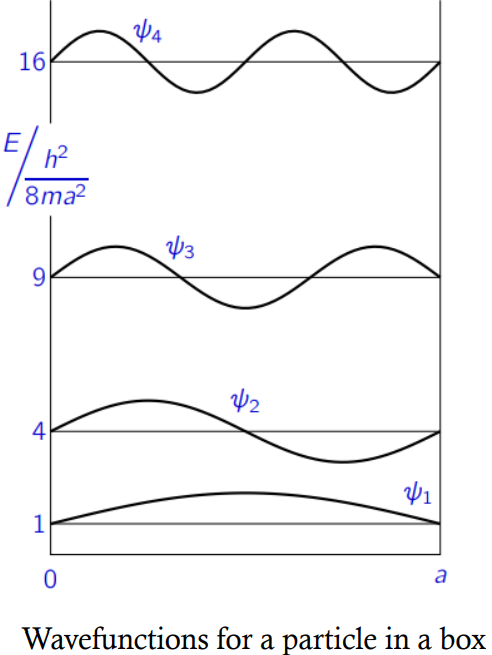
\includegraphics[scale=0.4]{fig/lzhx/微信图片_20211025150139.png}
\end{center}

\subsection{三维势箱Box[a,b,c]}
三维势箱在利用分离变量的方法可以看成三个一维势箱的乘积,这里我们简单介绍一下分离变量法在势箱中的应用,假设三维势箱三个坐标相互独立,则三维势箱波函数可以写成:
\[\varPsi(x,y,z):=X(x)Y(y)Z(z)\]
此时薛定谔方程可以展开为:
\[-\frac{\hbar^2}{2m}\nabla^2\varPsi=-\frac{\hbar^2}{2m}\left (YZ\frac{\partial^2X}{\partial x^2}+XZ\frac{\partial^2Y}{\partial y^2}+XY\frac{\partial^2Z}{\partial z^2} \right )=EXYZ\]

显然,除了平凡解$\psi=0$外,我们可以认为解出的波函数仅在有限个点上取值为零,不考虑这些奇异点,我们将方程两边同时除以$XYZ$:
\[-\frac{\hbar^2}{2m}\left (\frac{1}{X}\frac{\partial^2X}{\partial x^2}+\frac{1}{Y}\frac{\partial{d}^2Y}{\partial y^2}+\frac{1}{Z}\frac{\partial^2Z}{\partial z^2} \right )=E\]

同样的,我们定义:
\[E:=E_x+E_y+E_z\]

因此,我们可以将上述三维势箱薛定谔方程方程写成三个一维势箱薛定谔方程:
\[-\frac{\hbar^2}{2m}\frac{\mathrm{d}^2X}{\mathrm{d}x^2}=E_xX, \qquad -\frac{\hbar^2}{2m}\frac{\mathrm{d}^2Y}{\mathrm{d}y^2}=E_yY, \qquad -\frac{\hbar^2}{2m}\frac{\mathrm{d}^2Z}{\mathrm{d}z^2}=E_zZ\]

求解并合并得到三维势箱的波函数及能量:
\[\varPsi=\sqrt{\frac{8}{abc}}\sin\left (\frac{n_x \pi}{l}x \right )\sin\left (\frac{n_y \pi}{l}y \right )\sin\left (\frac{n_z \pi}{l}z \right ), \quad E_{x,n}=\frac{h^2}{8m} \left (\frac{n_x^2}{a^2}+\frac{n_y^2}{b^2}+\frac{n_z^2}{c^2} \right ) \quad (n_x,n_y,n_z \in \mathbb{N}_+)\]

\section{振动量子化——谐振子}
对势箱中的振动系统,我们可以把哈密顿量构造成:
\[\hat{H}=-\frac{\hbar^2}{2m_1}\nabla^2_1-\frac{\hbar^2}{2m_2}\nabla^2_2+V\]

对势能部分$V(r)$(内坐标表示),我们在平衡位置进行泰勒展开:
\[V(r)=V(r_e)+V^{'}(r)(r-r_e)+\frac{1}{2}V^{''}(r)(r-r_e)^2+\frac{1}{6}V^{'''}(r)(r-r_e)^3 \cdots=\sum_{i=0}^{+\infty}\frac{V^{(i)}(r_e)}{i!}(r-r_e)^i\]

对谐振子系统,其势能项可以为:
\[V(r)=V(r_e)+\frac{1}{2}V^{''}(r)(r-r_e)^2\]

因此,势箱中的谐振子薛定谔方程可以描述为:
\[\left (-\frac{\hbar^2}{2m_1}\nabla^2_1-\frac{\hbar^2}{2m_2}\nabla^2_2+V(r_e)+\frac{1}{2}V^{''}(r)(r-r_e)^2 \right )\varPsi=E\varPsi\]
考虑质心系
\[\left (-\frac{\hbar^2}{2\mu}\nabla^2+V(r_e)+\frac{1}{2}V^{''}(r)(r-r_e)^2 \right )\varPsi=E\varPsi\]

这里,我们不再求解该方程,有兴趣的可以自己上网查,这边直接给出解的形式:

则,解为:
\[\varPsi_n(x)=\left(\frac{\mu\omega}{\pi\hbar}\right)^{\frac{1}{4}}\frac{1}{\sqrt{2^nn!}}H_n(\sqrt{\frac{\mu\omega}{\hbar}}x)exp\left(-\frac{\mu\omega}{2\hbar}x^2\right) \qquad (n=1,2,3 \cdots)\]

能量为:
\[E_n=\left(n+\frac{1}{2}\right)h\nu=\left(n+\frac{1}{2}\right)\hbar\omega \qquad (n=1,2,3\cdots)\]

其中:
\[H_n(q)=(-1)^ne^{q^2}\frac{\mathrm{d}}{\mathrm{d}x}e^{-q^2} \qquad (n=1,2,3\cdots)\]
\[H_0(q)=1 \qquad H_1(q)=2q \qquad H_2(q)=4q^2-2\]
\[\omega=\sqrt{\frac{k}{\mu}}\]

当然,对一般的振动系统,谐振子近似经常是不够的,这时我们会引入非谐校正,比如,引入$Morse \ potential$:
\[V(r)=D_e\left[1-e^{-\beta(r-r_e)}\right]^2\]

同样对其进行展开得到:
\[V(r)=D_e\left[\beta^2(r-r_e)^2-\beta^3(r-r_e)^3+\cdots\right]\]

因此,对应于谐振子的力常数$k$有如下关系:
\[k=2\beta^2D_e\]

其能量可以用以下表达式给出:
\[E_\nu=\left(\nu+\frac{1}{2}\right)\hbar\omega-\left(\nu+\frac{1}{2}\right)^2\hbar\omega x_e \qquad x_e=\frac{\hbar\beta^2}{2\mu\omega}=\frac{\hbar\omega}{4D_e}\]

\begin{center}
    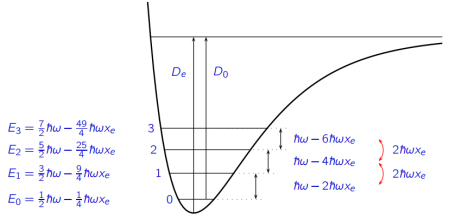
\includegraphics[scale=0.7]{fig/lzhx/微信图片_20211104112141.png}
\end{center}

\section{转动量子化——刚性转子}
由之前的讨论,我们知道,一个粒子的哈密顿量可以表示成:
\[\hat{H}=-\frac{\hbar^2}{2m}\nabla^2 + V=-\frac{\hbar^2}{2m}\left ( \frac{\partial^2}{\partial x^2}+\frac{\partial^2}{\partial y^2}+\frac{\partial^2}{\partial z^2}\right ) + V\]

因此,我们可以考虑两个粒子组成的刚性转子哈密顿量为:
\[\hat{H}=-\frac{\hbar^2}{2m}\left ( \frac{\partial^2}{\partial x_2^2}+\frac{\partial^2}{\partial y_2^2}+\frac{\partial^2}{\partial z_2^2}\right ) -\frac{\hbar^2}{2m}\left ( \frac{\partial^2}{\partial x_2^2}+\frac{\partial^2}{\partial y_2^2}+\frac{\partial^2}{\partial z_2^2}\right ) + V_{12}\]

考虑势箱中的刚性转子,$V_{12}=0$:
\[\hat{H}=-\frac{\hbar^2}{2m}\left ( \frac{\partial^2}{\partial x_1^2}+\frac{\partial^2}{\partial y_1^2}+\frac{\partial^2}{\partial z_1^2}\right ) -\frac{\hbar^2}{2m}\left ( \frac{\partial^2}{\partial x_2^2}+\frac{\partial^2}{\partial y_2^2}+\frac{\partial^2}{\partial z_2^2}\right )\]

定义内坐标:
\[ \left \{
    \begin{array}{ll}
        x=x_1-x_2  \\
        y=y_1-y_2  \\
        z=z_1-z_2
    \end{array}
    \right .
\]

则刚性转子的哈密顿量可以写成:
\[\hat{H}=-\frac{\hbar^2}{2}\left (\frac{1}{m_1}+\frac{1}{m_2}\right )\left ( \frac{\partial^2}{\partial x^2}+\frac{\partial^2}{\partial y^2}+\frac{\partial^2}{\partial z^2}\right )=-\frac{\hbar^2}{2\mu}\left ( \frac{\partial^2}{\partial x^2}+\frac{\partial^2}{\partial y^2}+\frac{\partial^2}{\partial z^2}\right ) \]

在球坐标下展开:
\[\hat{H}=-\frac{\hbar^2}{2\mu} \left (\frac{1}{r^2}\frac{\partial}{\partial{r}}(r^2\frac{\partial}{\partial{r}})+\frac{1}{r^2sin\theta}\frac{\partial}{\partial{\theta}}(sin\theta\frac{\partial}{\partial{\theta}})+\frac{1}{r^2sin^2 \theta }\frac{\partial^2}{\partial{\phi^2}} \right )\]

已知其中$r$为常数,则哈密顿量可以继续简化成:
\[\hat{H}=-\frac{\hbar^2}{2\mu} \left (\frac{1}{r^2sin\theta}\frac{\partial}{\partial{\theta}}(sin\theta\frac{\partial}{\partial{\theta}})+\frac{1}{r^2sin^2 \theta }\frac{\partial^2}{\partial{\phi^2}} \right )\]

将哈密顿量对波函数作用,我们稍作变形:
\[\hat{H}\varPsi=-\frac{\hbar^2}{2\mu} \left (\frac{1}{r^2sin\theta}\frac{\partial}{\partial{\theta}}(sin\theta\frac{\partial}{\partial{\theta}})+\frac{1}{r^2sin^2 \theta }\frac{\partial^2}{\partial{\phi^2}} \right )\varPsi=E\varPsi\]
\[-\hbar^2\left (\frac{1}{sin\theta}\frac{\partial}{\partial{\theta}}(sin\theta\frac{\partial}{\partial{\theta}})+\frac{1}{sin^2 \theta }\frac{\partial^2}{\partial{\phi^2}} \right )\varPsi=2\mu r^2 E\varPsi\]

稍微回顾一下经典力学,考虑两个质点$m_1$、$m_2$和轻轴组成的刚性旋转子,两质点间距为r,则此系统的质心系坐标、转动惯量和角动量及能量可以表示成:
\[r_1=\frac{m_2}{m_1+m_2}r \qquad r_2=\frac{m_1}{m_1+m_2}r\]
\[I=I_1+I_2=m_1r_1^2+m_2r_2^2=\frac{m_1m_2}{m_1+m_2}r^2\]
\[L=I\omega \qquad E=\frac{1}{2}I\omega^2=\frac{L^2}{2I}\]

则,我们可以将上述薛定谔方程改写成:
\[-\hbar^2\left (\frac{1}{sin\theta}\frac{\partial}{\partial{\theta}}(sin\theta\frac{\partial}{\partial{\theta}})+\frac{1}{sin^2 \theta }\frac{\partial^2}{\partial{\phi^2}} \right )\varPsi=L^2\varPsi\]

定义角动量平方算符,它反映的是波函数在空间中的角度部分延展程度:
\[\hat{J}^2=-\hbar^2\left (\frac{1}{sin\theta}\frac{\partial}{\partial{\theta}}(sin\theta\frac{\partial}{\partial{\theta}})+\frac{1}{sin^2 \theta }\frac{\partial^2}{\partial{\phi^2}} \right )\]

因此有:
\[\hat{J}^2\varPsi=L^2\varPsi\]

如果我们去解这个方程,我们会得到(我爬了,我实在不想再解一遍,想看的自己去附录求解氢原子薛定谔方程里找类似的部分,这里提供两个解的思路:一是级数法解微分方程,另外是利用升降算符):
\[\hat{J}^2\varPsi=l(l+1)\hbar^2\varPsi\]

其中$l$为角量子数。

当然,既然有了$\hat{J}^2$利用角动量模的平方表征波函数的角度部分,当然也会有利用角动量在某方向上的投影表征波函数的角度部分的算符,我们取投影方向为z:
\[\hat{J_z}\varPsi=l\hbar\varPsi\]

值得一提的是,量子力学中大部分算符是延用经典力学的算符,比如角动量算符可以通过$J=r \times p$得到。
 
\begin{center}
    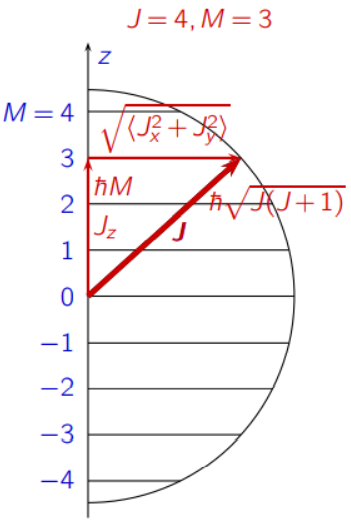
\includegraphics[scale=0.5]{fig/lzhx/微信图片_20211026130340.png}
\end{center}

\section{氢原子}
\subsection{氢原子薛定谔方程求解}
想看自己看第\ref{hydrgen}章。

\subsection{实、复轨道?}
举个例子,求解氢原子薛定谔方程我们能得到$n=2$,$l=1$,$m=-1,0,1$三个轨道波函数的表达式:
\[2p_0=N_{2p}ze^{-\frac{r}{2}} \qquad (m=0)\]
\[2p_1=-N_{2p}\frac{\sqrt{2}}{2}(x+iy)e^{-\frac{r}{2}} \qquad (m=1) \]
\[2p_{-1}=N_{2p}\frac{\sqrt{2}}{2}(x-iy)e^{-\frac{r}{2}} \qquad (m=-1) \]

这些轨道与我们所熟知的$2p_x,2p_y,2p_z$有如下关系:
\[2p_z=2p_0=N_{2p}ze^{-\frac{r}{2}} \quad 2p_x=\frac{\sqrt{2}}{2}(2p_{-1}-2p_1)=N_{2p}xe^{-\frac{r}{2}} \quad 2p_y=\frac{\sqrt{2}i}{2}(2p_{-1}+2p_1)=N_{2p}ye^{-\frac{r}{2}}\]

由于能量简并,这几个轨道的线性组合得到的任意波函数都是哈密顿量的本征函数,如果轨道能量不简并的话,轨道线性组合的结果将并不会是哈密顿量的本征函数,其对算符作用后得到的也不是本征值而是期望值。

\section{单核多电子体系}
\subsection{波恩-奥本海默(Born-Oppenheimer)近似}
理论上对于一个微观体系,只要我们确定了粒子组成及其相互作用,我们就能写出该体系的哈密顿量,利用基本假设薛定谔方程去求解体系的波函数。但是实际上你解个氢原子都解得要死要活的了,甚至氢分子你都不能给出解析解。那么引入一些近似在不降低太多准确度的前提下大幅提高计算的速度就显得尤为重要。这里我们将介绍一个最普遍的近似——波恩-奥本海默(BO)近似。

哈密顿量可以写成动能部分和势能部分,那么我们还能继续拆下去吗,该怎么拆呢?一个自然而然的想法就是我们能不能把核的运动和电子的运动分离开呢?于是我们就假设核跟电子的运动无关,进而可以将动能项拆成核动能部分和电子动能部分:
\[\hat{H}=\hat{T_n}+\hat{T_e}+\hat{V}=\hat{T_n}+\hat{H_e}=-\sum_i\frac{\hbar^2}{2m_{n,i}}\nabla^2_{n,i}-\sum_j\frac{\hbar^2}{2m_e}\nabla^2_{e,j}+\sum_{i,j}V_{i,j}\]

由于核的运动与电子的运动解耦,我们假设电子的波函数$\psi(\bm{Q},\bm{q})$和核的波函数$\varphi(\bm{Q})$可以分离,于是波函数可以写成如下形式,其中$\bm{Q}$为核坐标,$\bm{q}$为电子坐标:
\[\varPsi(\bm{Q},\bm{q})=\psi(\bm{Q},\bm{q})\varphi(\bm{Q})\]

由于解耦,对电子部分的薛定谔方程来说核坐标$\bm{Q}$被视为参数引入,电子可以感受到核对其的库仑力,这就意味着,反复求解不同核坐标微小变化下的电子薛定谔方程可以获得电子能量$U(\bm{Q})$关于核坐标$\bm{Q}$函数,成为势能面(PES)。由于这种将电子波函数重新计算为无穷小变化的核几何形状的函数的过程让人想起绝热定理的条件,因此这种获得 PES 的方式通常称为绝热近似,而 PES 本身称为绝热面。

正如BO近似的另一个名字定核近似,简单理解,电子相对于核运动太快,波恩-奥本海默近似就是认为核不动,当然这是不对的,\textcolor{blue}{\textbf{BO近似认为的是电子相较于原子核运动很快所以认为核坐标变化后电子总能在瞬间达到新的平衡}},所以有$\nabla^2_n\psi(\bm{Q},\bm{q}) \approx 0, \ \nabla_n\psi(\bm{Q},\bm{q}) \approx 0$。

将哈密顿量作用在波函数上,先看核动能部分:
\[\begin{aligned}
\hat{T_n}\varPsi(\bm{Q},\bm{q})&=-\sum_i\frac{\hbar^2}{2m_{n,i}}\left (\nabla^2_{n,i}\psi(\bm{Q},\bm{q}) \cdot \varphi(\bm{Q})+2\nabla_{n,i}\psi(\bm{Q},\bm{q}) \cdot \nabla_{n,i}\varphi(\bm{Q})+ \psi(\bm{Q},\bm{q}) \cdot \nabla^2_{n,i}\varphi(\bm{Q})  \right )\\ 
&\approx -\sum_i\frac{\hbar^2}{2m_{n,i}}\psi(\bm{Q},\bm{q}) \cdot \nabla^2_{n,i}\varphi(\bm{Q})=-\psi(\bm{Q},\bm{q})\sum_i\frac{\hbar^2}{2m_{n,i}}\nabla^2_{n,i}\varphi(\bm{Q})
\end{aligned}\]

考虑电子动能部分:
\[\hat{T_e}\varPsi(\bm{Q},\bm{q})=-\varphi(\bm{Q})\sum_j\frac{\hbar^2}{2m_e}\nabla^2_{e,j}\psi(\bm{Q},\bm{q})\]

合并整个哈密顿量,可以将薛定谔方程改写成如下形式:
\[\hat{H}\varPsi(\bm{Q},\bm{q})=-\psi(\bm{Q},\bm{q})\sum_i\frac{\hbar^2}{2m_{n,i}}\nabla^2_{n,i}\varphi(\bm{Q})-\varphi(\bm{Q})\sum_j\frac{\hbar^2}{2m_e}\nabla^2_{e,j}\psi(\bm{Q},\bm{q})+\sum_{i,j}V_{i,j}\psi(\bm{Q},\bm{q})\varphi(\bm{Q})=E\psi(\bm{Q},\bm{q})\varphi(\bm{Q})\]

利用分离变量获得电子薛定谔方程:
\[-\sum_j\frac{\hbar^2}{2m_e}\nabla^2_{e,j}\psi(\bm{Q},\bm{q})+\sum_{i,j}V_{i,j}\psi(\bm{Q},\bm{q})=U(\bm{Q})\psi(\bm{Q},\bm{q})\]
与核运动方程:
\[-\sum_i\frac{\hbar^2}{2m_{n,i}}\nabla^2_{n,i}\varphi(\bm{Q})=[E-U(\bm{Q})]\varphi(\bm{Q})\]

电子结构所关心的是电子薛定谔方程,解出给定核构型下的电子分布,而动力学关心的是核薛定谔方程,认为给定核构型下的电子结构是已知的。一个有意思的事是:我们求解氢原子的波函数时用的是只含电子项的薛定谔方程,但是我们依然说这个是精确解,这是为什么呢?\textcolor{blue}{\textbf{因为波恩-奥本海默近似本质上是假定变量可分离,因此对实际上确实可分离的体系这就不是一种近似}}。BO近似是必要的,毕竟三体以上的系统我们没法精确求解。

\subsection{平均场(Mean field)近似}
至此,在BO近似后,我们开始接触多电子体系,需要注意的是现在我们其实还是不能直接处理这样的多电子体系,主要的原因是电子-电子相互作用我们处理不了(本质上还是三体以上的系统没法精确求解),所以我们需要考虑进一步近似把多电子体系近似成我们能处理的单电子体系。

考虑一个多电子多核系统,其电子哈密顿量可以表示成:
\[\hat{H}=-\sum_{i}\frac{\hbar^2}{2m_i}\nabla^2_i+\sum_{i,j}\frac{q_iq_j}{4 \pi \varepsilon_0 r_{ij}}-\sum_i\frac{q_iq_n}{4 \pi \varepsilon_0 r_{i}}\]

在平均场近似下,把其他电子对某电子的双体算符$(\hat{V}_{ij})$平均成其他电子对该电子产生的势场$(\hat{V}_{i})$,此时体系哈密顿算符可以被拆分成单个粒子的哈密顿算符之和:
\[\hat{H}=\sum_{i}\hat{H}_{i} \qquad \text{where} \quad \hat{H}_i=-\frac{\hbar^2}{2m_i}\nabla^2_i+V_i\]

同理,电子波函数也可以近似成各个单电子波函数的乘积$\varPsi=\varPsi_1(\bm{q}_1)\varPsi_2(\bm{q}_2)\cdots$(这里先对波函数这样的拆分方法正确性按下不表),此时系统的总薛定谔方程可以被拆分成一系列的单体哈密顿方程:
\[\hat{H}_i\varPsi_i=\left( -\frac{\hbar^2}{2m_i}\nabla^2_i+\hat{V}_i \right)\varPsi_i=\varepsilon_i\varPsi_i\]

\subsection{粒子全同性与泡利不相容原理}
全同性应该是微观粒子与宏观物体最不同的地方之一。

简单来说,对两个宏观物体A、B,除了速度、位置外,我们还有大小、颜色之类的特征作为区分物体A、B,这也即表面在经典物理框架下,并没有全同性这一说法。但对于微观粒子A、B,我们似乎只有速度和位置这类无法区分粒子的可观测量。

而对微观粒子,你可以通过测量获得粒子的一个一个一个物理量,但是会发现你测量你舌头上的电子跟野兽先辈林檎上的电子也能测出一样的物理量,即使把你舌头上的电子和野兽先辈林檎上的电子调换一下,你的舌头和野兽先辈的林檎都还是安然无恙的,这也就是微观粒子的全同性。

接下来,我们的表述将在全同性这一微观粒子基本性质下展开。

首先定义对换算符$\hat{P}_{ij}$:
\[\hat{P}_{ij}\varPsi(\cdots,i,\cdots,j,\cdots)=\varPsi(\cdots,j,\cdots,i,\cdots)\]

基于全同性,就一个多粒子体系而言,我们调换一对同类型的粒子,显然其分布概率(经典物理量)并不会被改变(有经典对应的物理量在埃伦费斯特定理(Ehrenfest's theorem)的保证下符合经典物理的行为):
\[\begin{aligned}
|\varPsi(\cdots,i,\cdots,j,\cdots)|^2&=|\varPsi(\cdots,j,\cdots,i,\cdots)|^2 \\ 
\varPsi(\cdots,i,\cdots,j,\cdots)&=\pm\varPsi(\cdots,j,\cdots,i,\cdots)
\end{aligned}\]

依据上述描述,对换算符和哈密顿算符必然是对易的:
\[\qty[\hat{P}_{ij},\hat{H}]=0\]

对应,上述两种波函数行为,我们定义两类粒子——玻色子和费米子:
\[
    \begin{array}{lll}
        \text{Boson} & \varPsi(\cdots,i,\cdots,j,\cdots)=\varPsi(\cdots,j,\cdots,i,\cdots) & \text{symmetric} \\
        \text{Fermion} & \varPsi(\cdots,i,\cdots,j,\cdots)=-\varPsi(\cdots,j,\cdots,i,\cdots) & \text{antisymmetric}
    \end{array}
\]

两者在自旋(某种对称性)上有截然不同的特征:玻色子自旋为整数,费米子自旋为半整数。我们来看电子,电子是费米子,所以电子的波函数应该是反对称的。

当然除了一次换电子,我们也可以考虑一次对换多个电子,我们将其记为$\hat{P}_k$,称为置换算符,在线代的行列式部分中已经用到过该算符。利用置换算符我们还可以构造对称算符$\hat{S}$以及反对称算符$\hat{A}$,其中$\tau$为任意n元排列$k$的逆序数,$k$的个数为$n!$:
\[\hat{S}=\frac{1}{\sqrt{n!}}\sum_{k}\hat{P}_{k} \qquad \hat{A}=\frac{1}{\sqrt{n!}}\sum_{k}(-1)^{\tau}\hat{P}_{k}\]

用这两个算符,我们可以构造出多满足泡利不相容原理的玻色子或费米子体系的波函数,以双粒子双能级体系为例,粒子用$1,2$区分,能级用$a,b$区分,\textcolor{blue}{\textbf{注意这里我们引入标号只是为例我们书写方便并不代表微观粒子可以区分}}:
\[
    \begin{array}{ll}
        \text{Boson} & \hat{S}\varPsi_{ab}(1,2)=\frac{1}{\sqrt{2!}}[\varphi_a(1)\varphi_b(2)+\varphi_a(2)\varphi_b(1)]\\
        \text{Fermion} & \hat{A}\varPsi_{ab}(1,2)=\frac{1}{\sqrt{2!}}[\varphi_a(1)\varphi_b(2)-\varphi_a(2)\varphi_b(1)] 
    \end{array}
\]

考虑一件有意思的事情,如果所有粒子处于同一个量子态,玻色子和费米子会有什么样的行为?

我们这里继续使用上述的两个算符构造:
\[\hat{S}\varPsi_{1}(1,2,3 \cdots)=\frac{1}{\sqrt{n!}}\sum_{k}\hat{P}_{k}\varPsi_{1}(1,2,3 \cdots)=\frac{1}{\sqrt{n!}}\cdot n!\prod_{i=1}^n\varphi_1(i)=\sqrt{n!}\prod_{i=1}^n\varphi_1(i)\]
\[\hat{A}\varPsi_{1}(1,2,3 \cdots)=\frac{1}{\sqrt{n!}}\sum_{k}(-1)^{\tau}\hat{P}_{k}\varPsi_{1}(1,2,3 \cdots)=\frac{1}{\sqrt{n!}}\left (\frac{n!}{2}\prod_{i=1}^n\varphi_1(i)-\frac{n!}{2}\prod_{i=1}^n\varphi_1(i) \right )=0\]
这证明了我们为什么只“见过”波色子扎推在一个能级中,而费米子只能孤零零地处于各自不同的能级上。

\subsection{电子自旋}
非相对论量子力学体系下,电子自旋被认为是电子的内禀性质,强行跟轨道角动量类比得到:

\[
    \begin{array}{ll}
        \hat{J}(\hat{J_x},\hat{J_y},\hat{J_z}) & \hat{S}(\hat{S_x},\hat{S_y},\hat{S_z}) \\
        L=\sqrt{l(l+1)}\hbar & S=\sqrt{s(s+1)}\\
        i=0,1,2 \cdots & s=\frac{1}{2}\\
        J_z=m_l\hbar & S_z=m_s\hbar\\
        m_l - \text{magnetic number}, & m_s - \text{magnetic spin number},\\
        \hat{J}^2=\hat{J_x}^2+\hat{J_y}^2+\hat{J_z}^2 & \hat{S}^2=\hat{S_x}^2+\hat{S_y}^2+\hat{S_z}^2 \\
        \qty[\hat{J}^2,\hat{J_n}]=0 \ (n=x,y,z) & \qty[\hat{S}^2,\hat{S_n}]=0 \ (n=x,y,z)\\
        \qty[\hat{J_x},\hat{J_y}]=i\hbar\hat{J_z} & \qty[\hat{S_x},\hat{S_y}]=i\hbar\hat{S_z}\\
        \qty[\hat{J_z},\hat{J_x}]=i\hbar\hat{J_y} & \qty[\hat{S_z},\hat{S_x}]=i\hbar\hat{S_y}\\
        \qty[\hat{J_y},\hat{J_z}]=i\hbar\hat{J_x} & \qty[\hat{S_y},\hat{S_z}]=i\hbar\hat{S_x}
    \end{array}
\]

虽然电子的自旋被认为是电子场的自然结论,但我们不打算在这里介绍相对论量子力学(我暂时也不会)。
本小节我们只介绍电子自旋的一些物理性质并讨论其部分算符以及可观测量,在下一章节我们会介绍电子自旋对原子的物理性质如光谱的影响。

\begin{center}
    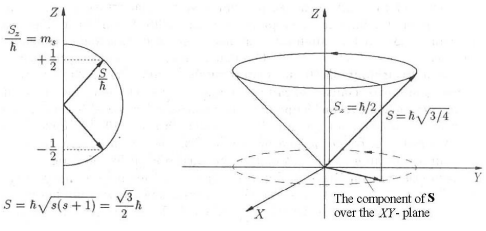
\includegraphics[scale=0.7]{fig/lzhx/微信图片_20211028113518}
\end{center}

总结一下我们至今碰到的算符,这里我们采用量子数形式的狄拉克表示符号代替波函数:
\[
    \begin{array}{ll}
        \ket{nlm_lm_s}=R_{nl}(r)Y_{l,m_l}(\theta,\varphi)\sigma_{m_s} \\
        \hat{H}\ket{nlm_lm_s}=E_{nl}\ket{nlm_lm_s} \\
        \hat{J}^2\ket{nlm_lm_s}=l(l+1)\hbar^2\ket{nlm_lm_s} \\
        \hat{J_z}\ket{nlm_lm_s}=m_l\hbar\ket{nlm_lm_s} \\
        \hat{S}^2\ket{nlm_lm_s}=s(s+1)\hbar^2\ket{nlm_lm_s} \\
        \hat{S_z}\ket{nlm_lm_s}=m_s\hbar\ket{nlm_lm_s}
    \end{array}
\]

如果我们对一个双电子体系进行考察,其自旋可以采用如下四种状态:
\[\sigma_{12}=\sigma_{1}\sigma_{2}=\alpha_1\alpha_2, \ \alpha_1\beta_2, \ \beta_1\alpha_2, \ \beta_1\beta_2\]

我们定义该体系的总自旋角动量z投影算符为:
\[\hat{S}_z=\hat{S}_{1z}+\hat{S}_{2z}\]

将其作用在该体系上:
\[\hat{S_z}\sigma_{12}=\hat{S_{1z}}\sigma_{1}\sigma_{2}+\hat{S_{2z}}\sigma_{1}\sigma_{2}=(m_{s1}+m_{s2})\sigma_{12}:=M_s\sigma_{12}\]

显然$M_s$可以取值$-1,0,1$,分别对应正交归一化波函数:
\[
    \left \{
    \begin{array}{ll}
        M_s=1  & \sigma_{12}=\alpha_1\alpha_2\\
        M_s=0  & \sigma_{12}=\alpha_1\beta_2,\beta_1\alpha_2\\
        M_s=-1 & \sigma_{12}=\beta_1\beta_2
    \end{array}
    \right .
\]

但总感觉上式有什么不对的地方。我们会发现当$M_s=0$时出现的自旋波函数对称性不满足我们在全同性中给出的要求(不对称的乘上什么都是不对称的),为此,我们需要讲这两个波函数进行线性组合使之满足对称性及归一化的要求,组合的合理性详见线性代数关于简并特征值的描述。

关于归一化,我们在这里补充一点说明,由于电子自旋假设,电子波函数可以写成,其中$\varphi$为轨道波函数,$\sigma$为自旋波函数,在之前的章节中,我们已经介绍了轨道波函数是归一的:
\[\varPsi=\varphi\sigma\]

介绍一种简单的表示方法——狄拉克表示:
\[
    \left \{
    \begin{array}{l}
        \bra{\varPsi}:=\varPsi^{*} \\
        \ket{\varPsi}:=\varPsi \\
        \bra{\varPsi}\hat{H}\ket{\varPsi}:=\int_E \varPsi^{*}\hat{H}\varPsi d\tau \\
        \bra{\varPsi}\ket{\varPsi}:=\int_E \varPsi^{*}\varPsi d\tau 
    \end{array} 
    \right .
\]
\[\bra{\varPsi}\ket{\varPsi}=\bra{\varphi\sigma}\ket{\varphi\sigma}=\bra{\varphi}\ket{\varphi}\bra{\sigma}\ket{\sigma}=1 \cdot 1=1\]

回到上述问题,我们假设:
\[\sigma_{0,1}=C_1\alpha_1\beta_2+C_2\beta_1\alpha_2 \qquad (C_1,C_2 \in \mathbb{R})\]

并构造$\sigma_{0,1}$的正交向量$\sigma_{0,2}$,在$\alpha_1\beta_2,\beta_1\alpha_2$张成的二维空间中,与$\sigma_{0,1}$正交的向量有且只有:
\[\sigma_{0,2}= \pm (C_1\alpha_1\beta_2-C_2\beta_1\alpha_2)\]

考虑常数的任意性,不妨取:
\[\sigma_{0,2}= C_1\alpha_1\beta_2-C_2\beta_1\alpha_2\]

$\sigma_{0,1}$、$\sigma_{0,2}$满足条件:
\[\bra{\sigma_{0,i}}\ket{\sigma_{0,i}}=C_1^2\bra{\alpha_1\beta_2}\ket{\alpha_1\beta_2}+C_2^2\bra{\beta_1\alpha_2}\ket{\beta_1\alpha_2}+2C_1C_2\bra{\alpha_1\beta_2}\ket{\beta_1\alpha_2}=C_1^2+C_2^2=1 \qquad (i=1,2)\]
\[\bra{\sigma_{0,1}}\ket{\sigma_{0,2}}=C_1^2\bra{\alpha_1\beta_2}\ket{\alpha_1\beta_2}-C_2^2\bra{\beta_1\alpha_2}\ket{\beta_1\alpha_2}=C_1^2-C_2^2=0\]

取系数$C_1$、$C_2$为正,得到:
\[\sigma_{0,1}=\frac{1}{\sqrt{2}}(\alpha_1\beta_2+\beta_1\alpha_2) \qquad \sigma_{0,2}= \frac{1}{\sqrt{2}}(\alpha_1\beta_2-\beta_1\alpha_2)\]

故$M_s$取值$-1,0,1$分别对应正交归一化波函数为:
\[ 
    \left \{
    \begin{array}{ll}
        M_s=1  & \sigma_{12}=\alpha_1\alpha_2\\
        M_s=0  & \sigma_{12}=\frac{1}{\sqrt{2}}(\alpha_1\beta_2+\beta_1\alpha_2),\frac{1}{\sqrt{2}}(\alpha_1\beta_2-\beta_1\alpha_2)\\
        M_s=-1 & \sigma_{12}=\beta_1\beta_2
    \end{array}
    \right .
\]
考虑对称性,我们可以讲上述四个轨道分为两类:
\[ 
    \begin{array}{ll}
        \text{symmetric}: & \text{antisymmetric}: \\
         \alpha_1\alpha_2\\
         \frac{1}{\sqrt{2}}(\alpha_1\beta_2+\beta_1\alpha_2) & \frac{1}{\sqrt{2}}(\alpha_1\beta_2-\beta_1\alpha_2)\\
         \beta_1\beta_2
    \end{array}
\]

类似于上述的讨论,关于双粒子的轨道波函数,我们也能构造出对称于反对称的正交归一波函数:
\[
    \begin{array}{ll}
        \text{symmetric}: & \text{antisymmetric}: \\
        \frac{1}{\sqrt{2!}}[\varphi_a(1)\varphi_b(2)+\varphi_a(2)\varphi_b(1)] & \frac{1}{\sqrt{2!}}[\varphi_a(1)\varphi_b(2)-\varphi_a(2)\varphi_b(1)] 
    \end{array}
\]

将两者组合,为满足电子波函数反对称化的要求,我们只能这么组合:
\[
    \begin{array}{l}
        \varPsi_{singlet}=\frac{1}{\sqrt{2!}}[\varphi_a(1)\varphi_b(2)+\varphi_a(2)\varphi_b(1)]\times\frac{1}{\sqrt{2}}(\alpha_1\beta_2-\beta_1\alpha_2)\\
        \varPsi_{triplet}=\frac{1}{\sqrt{2!}}[\varphi_a(1)\varphi_b(2)-\varphi_a(2)\varphi_b(1)]\times \left \{
            \begin{array}{l}
                \alpha_1\alpha_2\\
                \frac{1}{\sqrt{2}}(\alpha_1\beta_2+\beta_1\alpha_2)\\
                \beta_1\beta_2
            \end{array}
        \right .
    \end{array}
\]

至此,我们也顺便组合出了单重态和三重态的电子波函数。

\subsection{slater行列式}
slater行列式是一种构造反对称波函数的表示方式,这里以锂原子为例,数字为电子编号,其slater行列式为:
\[\varPhi=\frac{1}{\sqrt{n!}}
\left |
\begin{array}{lll}
1s(1)\alpha(1) & 1s(1)\beta(1) & 2s(1)\alpha(1) \\
1s(2)\alpha(2) & 1s(2)\beta(2) & 2s(1)\alpha(2) \\
1s(1)\alpha(3) & 1s(1)\beta(3) & 2s(1)\alpha(3)
\end{array}
\right |
=\frac{1}{\sqrt{n!}}
\left |
\begin{array}{lll}
1s(1) & \overline{1s(1)} & 2s(1) \\
1s(2) & \overline{1s(2)} & 2s(2) \\
1s(3) & \overline{1s(3)} & 2s(3)
\end{array}
\right |
\]

或者,我们可以换一种更简洁的表示方式:
\[\varPhi=\hat{A}\varPsi_{a_1,a_2,a_3 \cdots}(1,2,3\cdots)=\frac{1}{\sqrt{n!}}\sum_k(-1)^{\tau}\varPsi_{a_k}(k)\]

\subsection{氦原子}
根据上面的讨论,我们可以得到氦原子的$1s2s$激发单重态轨道波函数:
\[\varPsi_{+}=\frac{1}{\sqrt{2!}}[\varphi_a(1)\varphi_b(2)+\varphi_a(2)\varphi_b(1)]\]

久违地考虑一下能量,写出氦原子的电子哈密顿算符:
\[\hat{H}=-\sum_{i=1}^2\frac{\hbar^2}{2m_e}\nabla^2_i-\sum_{i=1}^2\frac{e^2}{2 \pi \varepsilon_0 r_{i}}+\frac{e^2}{4 \pi \varepsilon_0 r_{12}}\]

定义,球形势场下的单电子体系哈密顿算符为$\hat{h}$与能量$\varepsilon$,由之前的讨论我们知道该体系是可以精确求解的(下面的运算均在原子单位下表示,简洁):
\[E=\bra{\varPsi_{+}}\hat{H}\ket{\varPsi_{+}}=\bra{\varPsi_{+}}\hat{h}_1\ket{\varPsi_{+}}+\bra{\varPsi_{+}}\hat{h}_2\ket{\varPsi_{+}}+\bra{\varPsi_{+}}\frac{1}{r_{12}}\ket{\varPsi_{+}}=2\varepsilon_{1}+\bra{\varPsi_{+}}\frac{1}{r_{12}}\ket{\varPsi_{+}}\]

可以发现,阻止我们精确求解多电子体系的主要障碍来源于电子——电子相互作用项:
\[\bra{\varPsi_{+}}\frac{1}{r_{12}}\ket{\varPsi_{+}}\]

更准确的说是轨道——轨道相互作用,因为电子自旋部分与积分坐标无关且正交归一:
\[\bra{\varPsi_{+}}\frac{1}{r_{12}}\ket{\varPsi_{+}}=\bra{\varphi_{+}\sigma_{singlet}}\frac{1}{r_{12}}\ket{\varphi_{+}\sigma_{singlet}}=\bra{\varphi_{+}}\frac{1}{r_{12}}\ket{\varphi_{+}}\bra{\sigma_{singlet}}\ket{\sigma_{singlet}}=\bra{\varphi_{+}}\frac{1}{r_{12}}\ket{\varphi_{+}}\]

具体来看它:
\[\bra{\varphi_{+}}\frac{1}{r_{12}}\ket{\varphi_{+}}=\frac{1}{2}\int_{\mathbb{R}^{3 \times 2}}[\varphi_a(1)\varphi_b(2)+\varphi_a(2)\varphi_b(1)]^{*}\frac{1}{r_{12}}[\varphi_a(1)\varphi_b(2)+\varphi_a(2)\varphi_b(1)]d\tau_1d\tau_2\]
\[\bra{\varphi_{+}}\frac{1}{r_{12}}\ket{\varphi_{+}}=\int_{\mathbb{R}^{3 \times 2}} \left ( [\varphi_a(1)\varphi_b(2)]^{*}\frac{1}{r_{12}}[\varphi_a(1)\varphi_b(2)]+[\varphi_a(1)\varphi_b(2)]^{*}\frac{1}{r_{12}}[\varphi_a(2)\varphi_b(1)] \right )d\tau_1d\tau_2\]

定义库伦积分$J$和交换积分$K$,显然这两个积分都是正的:
\[J:=\int_{\mathbb{R}^{3 \times 2}}[\varphi_a(1)\varphi_b(2)]^{*}\frac{1}{r_{12}}[\varphi_a(1)\varphi_b(2)]d\tau_1d\tau_2\]
\[K:=\int_{\mathbb{R}^{3 \times 2}}[\varphi_a(1)\varphi_b(2)]^{*}\frac{1}{r_{12}}[\varphi_a(2)\varphi_b(1)]d\tau_1d\tau_2\]

可以看出,库伦积分与经典物理中的定义相符,而交换积分更像是经典物理中“凭空冒出来”的。

最后,我们得到:
\[\bra{\varPsi_{+}}\frac{1}{r_{12}}\ket{\varPsi_{+}}=J+K\]

对三重态:
\[\varPsi_{-}=\frac{1}{\sqrt{2!}}[\varphi_a(1)\varphi_b(2)-\varphi_a(2)\varphi_b(1)]\]

同理有:
\[\bra{\varPsi_{-}}\frac{1}{r_{12}}\ket{\varPsi_{-}}=J-K\]

可见同电子排布下,三重态能量一般是要比单重态低,验证洪特规则。

观察三重态和单重态波函数分布概率对$r_{12}$变化的行为:
\begin{center}
    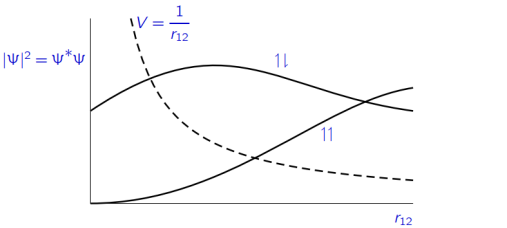
\includegraphics[scale=0.8]{fig/lzhx/微信图片_20211030111438.png}
\end{center}

在7.3中我们已经介绍了当$r_{12}=0$时的情况,三重态电子在$r_{12}=0$时分布概率为0,且从图像上来看,自旋平行的电子在空间上倾向于相互远离。而单重态电子在$r_{12}=0$时仍有分布,最大分布概率对应的$r_{12}$存在,也即我们一般认识的轨道半径。三重态在$r_{12}=0$的情况被称作Fermi hole。

\section{原子光谱}
对于原子的实际哈密顿量$\hat{H}$,我们可以把它拆成以下三个部分:平均场近似下的$\hat{H}_0$,平均场近似带来的与实际哈密顿量的势能误差项$\hat{H}^{'}$,以及填入电子后电子自旋与轨道自旋耦合带来的哈密顿量$\hat{H}_{SO}$。
\[\hat{H_0}=-\frac{\hbar^2}{2m_e}\sum_i\nabla^2_i+\sum_iV_i\]
\[\hat{H}^{'}=\sum_{i,j}\frac{1}{r_{ij}}-\sum_iV_i\]
\[\hat{H}_{SO}=\sum_{i}\xi(r_i)\hat{L}_i \cdot \hat{S}_i\]

旋轨耦合来源于哪里?其源头来自于量子纠缠,在原子分子尺度下,组成其的微粒——原子核/电子的德布罗意波强烈耦合,波函数无法独立区分,体系的物理量不能通过每个粒子的物理量进行加和得到。
\[\Psi(x_1,x_2) \neq \psi(x_1)\psi(x_2) \qquad \hat{A}\Psi(x_1,x_2) \neq (\hat{A}_1+\hat{A}_2)\psi(x_1)\psi(x_2)=(a_1+a_2)\psi(x_1)\psi(x_2)\]

表示方法(光谱项,光谱支项):
\[^{2S+1}L \qquad ^{2S+1}L_J\]

其中:
\[S=\sum_i\overrightarrow{m_s}(i)\]
\[L=\sum_i\overrightarrow{m_l}(i)\]
\[\overrightarrow{J}=\overrightarrow{S}+\overrightarrow{L} \qquad J=L+S,L+S-1,\cdots |L-S|\]

光谱支项多重度:
\[(2S+1)(2L+1)\]

每个光谱支项的简并度:
\[m_j:=2J+1\]

\subsection{Hund规则}
1、同电子组态,S越大越稳定;

2、S相同,L越大越稳定;

3、L、S相同,若电子数小于半满,J越小越稳定;若电子数大于半满,J越大越稳定。

\section{多核粒子体系——线性变分法}
对一些复杂的多核粒子体系,我们没有办法通过精确求解薛定谔方程得到其能量与波函数,但是我们可以通过利用现有的精确求解波函数猜测其实际波函数的办法来近似实际体系。
一般而言自然体系都会倾向于使得某态的能量尽可能低,所以我们可以利用猜测轨道得到的能量来衡量近似的质量。
当然该不等式可能需要要求猜测波函数是正交归一的。
\[\expval{\tilde{E}}=\frac{\bra{\varPhi}\hat{H}\ket{\varPhi}}{\bra{\varPhi}\ket{\varPhi}} \geqslant E_0\]

这里介绍一下基于原子轨道线性组合(LCAO)得到的猜测分子波函数LCAO-MO进行变分的过程,选用线性组合主要也是因为运算简单。

利用态叠加原理,现定义猜测波函数$\varPhi$,下表达式中,$c_i$为系数,$f_i$为已知波函数,波函数组张成的空间称为变分空间:
\[\varPhi=\sum_ic_if_i\]

代入我们的判据:
\[\expval{\tilde{E}}=\frac{\sum_{i,j}c_ic_j\bra{f_i}\hat{H}\ket{f_j}}{\sum_{i,j}c_ic_j\bra{f_i}\ket{f_j}}\]

这里再定义几个符号:
\[H_{ij}:=\bra{f_i}\hat{H}\ket{f_j} \qquad S_{ij}:=\bra{f_i}\ket{f_j} \qquad \sum:=\sum_{i,j}\]

则:
\[\expval{\tilde{E}}=\frac{\sum c_ic_jH_{ij}}{\sum c_ic_jS_{ij}}\]

为了找到再已有函数下使得$\expval{\tilde{E}}$最小的系数组$c_i$,我们需要$\expval{\tilde{E}}$对系数组$c_i$的偏导值等于0,二阶偏导矩阵正定。

为方便处理,我们做以下变形:
\[\expval{\tilde{E}}\sum c_ic_jS_{ij}=\sum c_ic_jH_{ij}\]

对$c_i$求偏导:
\[\frac{\partial \expval{\tilde{E}}}{\partial c_i}\sum c_ic_jS_{ij}+2\expval{\tilde{E}}\sum_j c_jS_{ij}=2\sum_j c_jH_{ij}\]
\[\frac{\partial \expval{\tilde{E}}}{\partial c_i}=\frac{2}{\sum c_ic_jS_{ij}}\left(\sum_j c_jH_{ij}-\expval{\tilde{E}}\sum_j c_jS_{ij}\right)=\frac{2}{\sum c_ic_jS_{ij}}\left(\sum_j \left (H_{ij}-\expval{\tilde{E}}S_{ij}\right )c_j\right)\]
\[\frac{\partial \expval{\tilde{E}}}{\partial c_i}=0 \Leftrightarrow \sum_j \left (H_{ij}-\expval{\tilde{E}}S_{ij}\right )c_j=0 \qquad (i=1,2,3 \cdots)\]

合并上式:
\[
\begin{pmatrix}
H_{11}-\expval{\tilde{E}}S_{11} & H_{12}-\expval{\tilde{E}}S_{12} & \ldots & H_{1n}-\expval{\tilde{E}}S_{1n}\\
H_{21}-\expval{\tilde{E}}S_{21} & H_{22}-\expval{\tilde{E}}S_{22} & \ldots & H_{2n}-\expval{\tilde{E}}S_{2n}\\
\vdots & \vdots & \ddots & \vdots\\
H_{n1}-\expval{\tilde{E}}S_{n1} & H_{n2}-\expval{\tilde{E}}S_{n2} & \ldots & H_{nn}-\expval{\tilde{E}}S_{nn}\\
\end{pmatrix}
\begin{pmatrix}
c_1\\
c_2\\
\vdots\\
c_n\\
\end{pmatrix}
=0
\]

要使得上述齐次方程有解,需要其系数矩阵行列式为0:
\[
    \begin{vmatrix}
        H_{11}-\expval{\tilde{E}}S_{11} & H_{12}-\expval{\tilde{E}}S_{12} & \ldots & H_{1n}-\expval{\tilde{E}}S_{1n}\\
        H_{21}-\expval{\tilde{E}}S_{21} & H_{22}-\expval{\tilde{E}}S_{22} & \ldots & H_{2n}-\expval{\tilde{E}}S_{2n}\\
        \vdots & \vdots & \ddots & \vdots\\
        H_{n1}-\expval{\tilde{E}}S_{n1} & H_{n2}-\expval{\tilde{E}}S_{n2} & \ldots & H_{nn}-\expval{\tilde{E}}S_{nn}\\
    \end{vmatrix}
    =0
\]

求解上述行列式我们能得到能量的估计最小值$\expval{\tilde{E}}$。

下面举个例子,如果我们考虑两个波函数张成的变分空间的线性变分:
\[\varPhi=\sum_{i=1}^2c_if_i\]
\[\expval{\tilde{E}}=\frac{\sum c_ic_jH_{ij}}{\sum c_ic_jS_{ij}}\]
\[\expval{\tilde{E}}\sum_{i=1}^2 c_ic_jS_{ij}=\sum_{i=1}^2 c_ic_jH_{ij}\]

对$c_i$求偏导:
\[\frac{\partial \expval{\tilde{E}}}{\partial c_i}\sum c_ic_jS_{ij}+2\expval{\tilde{E}}\sum_{i=1}^2 c_jS_{ij}=2\sum_{i=1}^2 c_jH_{ij}\]
\[\frac{\partial \expval{\tilde{E}}}{\partial c_i}=\frac{2}{\sum c_ic_jS_{ij}}\left(\sum_{i=1}^2 c_jH_{ij}-\expval{\tilde{E}}\sum_{i=1}^2 c_jS_{ij}\right)=\frac{2}{\sum c_ic_jS_{ij}}\left(\sum_j \left (H_{ij}-\expval{\tilde{E}}S_{ij}\right )c_j\right)\]
\[\frac{\partial \expval{\tilde{E}}}{\partial c_i}=0 \Leftrightarrow \sum_{i=1}^2 \left (H_{ij}-\expval{\tilde{E}}S_{ij}\right )c_j=0 \qquad (i=1,2)\]
\[
\begin{pmatrix}
H_{11}-\expval{\tilde{E}}S_{11} & H_{12}-\expval{\tilde{E}}S_{12} \\
H_{21}-\expval{\tilde{E}}S_{21} & H_{22}-\expval{\tilde{E}}S_{22} \\
\end{pmatrix}
\begin{pmatrix}
c_1\\
c_2
\end{pmatrix}
=0
\]
\[
    \begin{vmatrix}
        H_{11}-\expval{\tilde{E}}S_{11} & H_{12}-\expval{\tilde{E}}S_{12} \\
        H_{21}-\expval{\tilde{E}}S_{21} & H_{22}-\expval{\tilde{E}}S_{22} \\
    \end{vmatrix}
    =0
\]

对同核双原子分子,重新定义几个符号:
\[\alpha:=H_{11}=H_{22} \qquad \beta:=H_{12}=H_{21} \qquad S:=S_{12}=S_{21} \qquad S_{11}=S_{22}=1\]
\[
    \begin{vmatrix}
        \alpha-\expval{\tilde{E}} & \beta-\expval{\tilde{E}}S \\
        \beta-\expval{\tilde{E}}S & \alpha-\expval{\tilde{E}} \\
    \end{vmatrix}
    =0
\]

整理得到:
\[\alpha-\expval{\tilde{E}}=\pm (\beta-\expval{\tilde{E}}S)\]
\[\expval{\tilde{E}}=\frac{\alpha-\beta}{1-S} \ or \ \frac{\alpha+\beta}{1+S}\]

两个能量分别反带回去得到轨道:
\[\varPhi=\frac{1}{\sqrt{2+2S}}(\varPsi_1+\varPsi_2) \ when \ \expval{\tilde{E}}=\frac{\alpha-\beta}{1-S}\] 
\[\varPhi=\frac{1}{\sqrt{2-2S}}(\varPsi_1-\varPsi_2) \ when \ \expval{\tilde{E}}=\frac{\alpha+\beta}{1+S}\]

现在我们关注一下这两个轨道在空间中的分布情况:
\[\rho=\int_{\mathbb{R^3}}|\varPhi|^2d\tau\]
\[\rho_+=\frac{1}{2+2S}\int_{\mathbb{R^3}}\left(\varPsi_1^2+\varPsi_2^2+2\varPsi_1\varPsi_2\right) d\tau\quad \text{when} \ \varPhi=\frac{1}{\sqrt{2+2S}}(\varPsi_1+\varPsi_2)\] 
\[\rho_-=\frac{1}{2-2S}\int_{\mathbb{R^3}}\left(\varPsi_1^2+\varPsi_2^2-2\varPsi_1\varPsi_2\right) d\tau\quad \text{when} \ \varPhi=\frac{1}{\sqrt{2-2S}}(\varPsi_1-\varPsi_2)\]

值得注意的是,这两个能量其实并不好直接看出相对高低,需要直接计算,注意$\alpha,\beta,S$的数值大小。
但是在波函数上我们可以有更简单的判断方法——通过数节点数,节点数越多,波函数变化越剧烈,动能部分的能量也越高,根据位里定理(第二章)能量也就越高。

\begin{figure}[htbp]
    \centering
    \begin{minipage}[t]{0.48\textwidth}
    \centering
    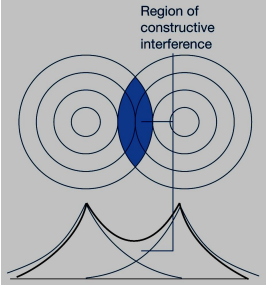
\includegraphics[width=5cm]{fig/lzhx/微信图片_20211102112346.png}
    \caption{$\rho_+$的分布图像}
    \end{minipage}
    \begin{minipage}[t]{0.48\textwidth}
    \centering
    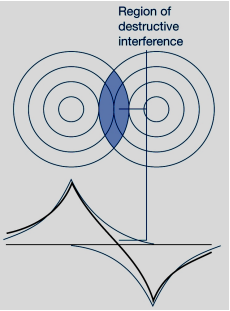
\includegraphics[width=5cm]{fig/lzhx/微信图片_202111021123461.png}
    \caption{$\rho_-$的分布图像}
    \end{minipage}
\end{figure}

有意思的是,如果考虑了重叠积分,组成的分子轨道上升的能量比下降的多:
\[\Delta E=\left(\frac{\alpha-\beta}{1-S}-\alpha\right)-\left(\alpha-\frac{\alpha+\beta}{1+S}\right)=2S \cdot \frac{\alpha S-\beta}{1-S^2}\]

考虑重叠积分$S$一般比较小,做小量分析,原式$\sim 2S \cdot (-\beta)>0$

\section{计算化学入门前的垫脚石上的艹}
\subsection{Hartree-Fock方法}
我们都知道一个孤立微观系统的哈密顿如下:
\[\hat{H}=\hat{T}_N+\hat{T}_e+\hat{V}_{Ne}+\hat{V}_{ee}+\hat{V}_{NN}\]
在BO近似后,$\hat{T}_N$从电子哈密顿中被移除,$\hat{V}_{NN}$给定核位置后是个常数,可以不包含在电子哈密顿中,但一般来说都还是算的。
\[\hat{H}_{el}=\hat{T}_e+\hat{V}_{Ne}+\hat{V}_{ee}+\hat{V}_{NN}=\sum_i\left(-\frac{1}{2}\nabla^2_i+\sum_N\frac{Z}{r_{Ni}}\right)+\sum_{i<j}\frac{1}{r_{ij}}+V_{NN}\]

虽然我们已经把核项给舍去了,但电子部分的哈密顿依然是一个多体哈密顿,还是一个难以求解的问题。
我们一般能处理的都是单体问题,比如氢原子的电子薛定谔、谐振子等等,所以我们希望能将多体问题尽可能精确地转换为单体问题来处理,如我们考虑平均场近似,即将其他电子对该电子的两体作用考虑为一个等效场:
\[\hat{H}_{el} \approx \sum_i\left(-\frac{1}{2}\nabla^2_i+\sum_N\frac{Z}{r_{Ni}}+\hat{v}_i\right)+V_{NN}:=\sum_i\hat{F}_i + V_{NN}\]

如此一来,上述多电子问题就被转换为了单电子问题,多体哈密顿量被转换单体哈密顿量的加和,理所当然,该体系的波函数也变成了几个单体波函数(自旋轨道)的乘积Hartree积:
\[\Psi = \psi_1(1)\psi_2(2)\cdots\psi_n(n)=\prod_i\psi_i(i)\]

由于电子费米子的全同性的要求,上述需要对Hartree基做反对称化得到Slater行列式:
\[\Psi=\frac{1}{\sqrt{n!}}
    \begin{vmatrix}
        u_1(1) & u_2(1) & \ldots & u_n(1)\\
        u_1(2) & u_2(2) & \ldots & u_n(2)\\
        \vdots & \vdots & \ddots & \vdots\\
        u_1(n) & u_2(n) & \ldots & u_n(n)\\
    \end{vmatrix}
\]

可以看到上面我们假定了单体波函数组成的体系波函数是精确的,然后认为哈密顿量是不精确的,由此出发,我们会希望通过不断修正哈密顿量来使得结果更精确,于是就有了MP2、MP4等微扰方法的出现。
另一方面,如果我们认为哈密顿量是精确的,那么就认为波函数是不精确的,从Slater行列式出发我们通过变分方法来求解尽可能精确的波函数,已知能量表达式为:
\[E=\frac{\bra{\Psi}\hat{H}\ket{\Psi}}{\bra{\Psi}\ket{\Psi}}\]

体系波函数满足:
\[\bra{u_i(1)}\ket{u_j(1)}=\delta_{ij}\]

体系哈密顿量为:
\[\hat{H}=\sum_i\left(-\frac{1}{2}\nabla^2_i+\sum_N\frac{Z}{r_{Ni}}\right)+\sum_{i<j}\frac{1}{r_{ij}}+V_{NN}\]

由Condon-Slater规则可知,能量$E$如下所示,其中$\bra{ij}\ket{ij},\bra{ij}\ket{ji}$为库伦积分和交换积分,$\hat{h}_i$包括了动能项和核对电子的势能(单体算符):
\[E=\bra{\varPhi}\hat{H}\ket{\varPhi}=\sum_ih_i+\frac{1}{2}\sum_{i,j}\left(\bra{ij}\ket{ij}-\bra{ij}\ket{ji}\right)\]

得到了能量,我们接下来顺理成章的就该来变分,但这里的变分并不是简单的求极值,而是条件变分,由于波函数的限制我们求变分时需要引入以下条件进行拉格朗日乘数法:
\[\bra{u_i(1)}\ket{u_j(1)}-\delta_{ij}=0\]

定义泛函$\eta(\lambda_{ij})$:
\[\eta(\lambda_{ij})=E+\sum_{i,j}\lambda_{ij}(\bra{u_i(1)}\ket{u_j(1)}-\delta_{ij})\]

由(变分计算量太大而且其他书上有,我就不写了):
\[\frac{\delta\eta(\lambda_{ij})}{\delta u_i}=\frac{\delta}{\delta u_i}\left(E+\sum_{i,j}\lambda_{ij}(\bra{u_i(1)}\ket{u_j(1)}-\delta_{ij})\right)=0\]

得到的变分结果我们记为:
\[\hat{F}\varphi_i=\varepsilon_i\varphi_i \qquad \varepsilon_i=\bra*{u_i}\hat{h} + \hat{J} - \hat{p}\ket*{u_i}\]

其中,$\hat{F}$为Fork算符,$\varepsilon_i$为轨道能量,$\varphi_i$为正则自旋轨道,Fork算符表达式为:
\[\hat{F} = \hat{h} + \hat{J} - \hat{p}\]
\[\hat{J}u_i(1) = \sum_{j \neq i}\left(\int u_j^*(2)\frac{1}{r_{ij}}u_j(2)d\tau_2\right)u_i(1) \qquad \hat{p}u_i(1) = \sum_{j \neq i}\left(\int u_j^*(2)\frac{1}{r_{ij}}u_i(2)d\tau_2\right)u_j(1)\]

Hartree-Fork能量如下给出,可以看到其不等于轨道能量之和,原因是因为考虑了电子之间的相互作用。

\[E_{HF}=\sum_ih_i+\frac{1}{2}\sum_{i,j}\left(\bra{ij}\ket{ij}-\bra{ij}\ket{ji}\right)+V_{NN}\]

当然,单个Slater行列式描述一个多体问题也是有误差的,于是我们希望能进一步地精确波函数,于是就有了CI、CC等方法。

话说回来,由于我们还是给不出每一个自旋轨道的解析式,所以这个方法我们还没办法直接用。

\subsection{Hartree-Fock–Roothaan方法}
如上文所说,我们给不出Hartree-Fock方程所需的体系波函数,所以我们需要用已知的函数去拟合体系波函数,这里给出Roothaan给出的方法,得到的方程称为Hartree-Fock–Roothaan方程:

假定体系波函数可以被已知基组展开,下面的公式中同时会展示矩阵表示,基向量采用行向量表示:
\[\psi_i=\sum_{\nu=1}c_{\nu i}f_{\nu} \qquad (\mathbf{\Psi} = \mathbf{\Phi} \mathbf{C}_{\text{coeff}})\]
将基函数带入Hartree-Fock方程后可以得到如下表达式:
\[\hat{F}\sum_{\nu=1}c_{\nu i}f_{\nu}=\varepsilon_i\sum_{\nu=1}c_{\nu i}f_{\nu}\]
对上述方程等式两边同时左乘一个$f_{\mu}$可以得到
\[\sum_{\nu=1}c_{\nu i}\bra{f_{\mu}}\hat{F}\ket{f_{\nu}}=\varepsilon_i\sum_{\nu=1}c_{\nu i}\bra{f_{\mu}}\ket{f_{\nu}} \quad \text{where} \quad F_{rs}=\bra{f_r}\hat{F}\ket{f_s} \quad \text{and} \quad S_{rs}=\bra{f_r}\ket{f_s}\]

如果把所有波函数都做上述展开,则可写成如下Hartree-Fock–Roothaan方程
\[\mathbf{F}\mathbf{C}=\mathbf{S}\mathbf{C}\varepsilon\]

上述方程组似乎跟我们能解的方程有一点点不一样,我们能处理的是方程组是厄密矩阵(这里是实对称阵)的正交对角化的问题:
\[\mathbf{F}\mathbf{C}'=\mathbf{C}'\varepsilon\]

Fock矩阵也是实对称矩阵,overlap矩阵也是实对称矩阵,我们自然会想到能不能将Hartree-Fock–Roothaan方程转化成上述方程呢?
考虑如下基的酉变换:
\[\phi_i = \sum_{i}U_{ji}f_j \qquad \mathbf{\varPhi}=\mathbf{U}\mathbf{\Psi}\]
其中$\mathbf{U}$为
\[\mathbf{U}=\mathbf{X}\mathbf{s}^{-1/2} \qquad \mathbf{X}^{\dagger}\mathbf{S}\mathbf{X}=\mathbf{s}\]
$\mathbf{X}$,$\mathbf{s}$为$\mathbf{S}$正交对角化的变换矩阵和对角阵,$\mathbf{s}^{-1/2}$为矩阵$\mathbf{s}^{-1}$的开放,其定义为$\mathbf{s}^{-1/2}\mathbf{s}^{-1/2}=\mathbf{s}^{-1}$。

做完如下变换之后,Hartree-Fock–Roothaan方程可以改写成:
\[\mathbf{U}^{\dagger}\mathbf{S}\mathbf{U}\mathbf{C}'=(\mathbf{X}\mathbf{s}^{-1/2})^{\dagger}\mathbf{S}(\mathbf{X}\mathbf{s}^{-1/2})\mathbf{C}'=\mathbf{X}^{\dagger}\mathbf{S}\mathbf{X}\mathbf{s}^{-1}\mathbf{C}'=\mathbf{s}\mathbf{s}^{-1}\mathbf{C}'=\mathbf{C}' \ , \ (\mathbf{C}':=\mathbf{U}^{\dagger}\mathbf{C})\]
\[\mathbf{U}^{\dagger}\mathbf{F}\mathbf{U}\mathbf{C}'=\varepsilon\mathbf{C}' \Rightarrow \mathbf{F}'\mathbf{C}'=\varepsilon\mathbf{C}' \ , \ (\mathbf{F}':=\mathbf{U}^{\dagger}\mathbf{F}\mathbf{U})\]

然后我们就能解这样一个变换后的方程了。
实际上在python中使用scipy.linalg.eigh($\mathbf{F}$,$\mathbf{S}$)就能直接解出$\mathbf{C}$。
但求解Hartree-Fock–Roothaan方程真的只是做一个对角化吗,如果是这样就好了。
我们具体来看每个矩阵的具体形式,系数矩阵和overlap矩阵是简单的,fock矩阵包含了单电子积分和双电子积分:
\[F_{\mu\nu} = \bra*{\phi_{\mu}}\hat{h} + \hat{J} - \hat{p}\ket*{\phi_{\nu}}\]
单电子积分是简单的
\[h_{\mu\nu}=\bra*{\phi_{\mu}}\hat{h}\ket*{\phi_{\nu}}\]
双电子积分我们打包处理
\begin{equation*}
    \begin{aligned}
        \bra*{\phi_{\mu}}\hat{J} - \hat{p}\ket*{\phi_{\nu}} & = \bra*{\phi_{\mu}}\ket{\sum_{j \neq i}\left(\int u_j^*(2)\frac{1}{r_{ij}}u_j(2)\dd{\tau_2}\right)\phi_{\nu}(1)-\sum_{j \neq i}\left(\int u_j^*(2)\frac{1}{r_{ij}}\phi_{\nu}(2)\dd{\tau_2}\right)u_j(1)} \\
         & = \sum_{j}\iint \phi_{\mu}^*(1)u_j^*(2)\left[\frac{1}{r_{ij}}(1-\hat{P}_{12})\right]u_j(2)\phi_{\nu}(1) \dd{\tau_1}\dd{\tau_2} \\
         & = \sum_{\alpha}\sum_{\beta}\sum_{j}c^*_{\alpha j}c_{\beta j}\iint \phi_{\mu}^*(1)\phi_{\alpha}^*(2)\left[\frac{1}{r_{ij}}(1-\hat{P}_{12})\right]\phi_{\beta}(2)\phi_{\nu}(1) \dd{\tau_1}\dd{\tau_2} \\
         & := \sum_{\alpha}\sum_{\beta}D_{\alpha\beta}\iint \phi_{\mu}^*(1)\phi_{\alpha}^*(2)\left[\frac{1}{r_{ij}}(1-\hat{P}_{12})\right]\phi_{\beta}(2)\phi_{\nu}(1) \dd{\tau_1}\dd{\tau_2} \\
         & := \sum_{\alpha}\sum_{\beta}D_{\alpha\beta}\bra{\phi_{\mu}\phi_{\alpha}}\ket{|\phi_{\nu}\phi_{\beta}}
    \end{aligned}
\end{equation*}
其中$D_{\alpha\beta}$是密度矩阵的矩阵元,显然我们知道密度矩阵可以由系数矩阵得到$\mathbf{D}=\mathbf{C}\mathbf{C}^{\dagger}$,所以事实上,我们得到的类似矩阵对角化的一个方程实际上也不像是看起来的那么简单,对这样的方程我们没办法直接求解,于是我们选择万能的迭代。
迭代需要一个初猜,在这里也就是初始的密度矩阵(给初猜也是技术活),然后通过对角化更新密度矩阵,反复迭代直到密度矩阵不再变化,这也就是SCF过程。
\[\mathbf{F}(\mathbf{C}')\mathbf{C}'=\mathbf{C}'\varepsilon\]

关于Hartree-Fock方法更多的内容推荐大家阅读\textbf{Szabo前三章},也希望各位能够自己写一个程序来实现(doge),这里提供两个实例:
\href{https://github.com/yangdatou/hf-tutorial}{大头版HF (积分算好了) }和
\href{https://github.com/Walter-Feng/Hartree-Fock-in-CPP}{叔叔版HF (从基组开始嗯造)}。

Hartree-Fock–Roothaan方程还有另外一个形式,以密度矩阵形式体现
\[\mathbf{F}\mathbf{P}\mathbf{S}=\mathbf{S}\mathbf{P}\mathbf{F}\]

证明上述方程与Hartree-Fock–Roothaan方程等价之前先介绍密度矩阵的几个性质
\[1. \ \mathbf{P}=\mathbf{P}^{\dagger} \qquad 2. \ \mathbf{P}\mathbf{S}\mathbf{P}=\mathbf{P} \qquad 3.\ \text{Tr}(\mathbf{P}\mathbf{S})=N\]

开始证明
\[\mathbf{F}\mathbf{C}=\varepsilon\mathbf{S}\mathbf{C} \quad \Rightarrow \quad \mathbf{F}\mathbf{C}(\mathbf{S}\mathbf{C})^{\dagger}=\varepsilon\mathbf{S}\mathbf{C}(\mathbf{S}\mathbf{C})^{\dagger} \quad \Rightarrow \quad \mathbf{F}\mathbf{P}\mathbf{S}=\varepsilon\]
\[\mathbf{F}\mathbf{C}=\varepsilon\mathbf{S}\mathbf{C} \quad \Rightarrow \quad \mathbf{F}\mathbf{C}(\mathbf{F}\mathbf{C})^{\dagger}=\varepsilon\mathbf{S}\mathbf{C}(\mathbf{F}\mathbf{C})^{\dagger} \quad \Rightarrow \quad \mathbf{I}=\varepsilon\mathbf{S}\mathbf{P}\mathbf{F} \quad \Rightarrow \quad \mathbf{I}=(\varepsilon\mathbf{S}\mathbf{P}\mathbf{F})^{\dagger} \quad \Rightarrow \quad \mathbf{S}\mathbf{P}\mathbf{F}=\varepsilon^{\dagger}=\varepsilon\]

基于上述形式的自洽场方程可以介绍DIIS辣!


\subsection{部分基组}
\paragraph*{Slater-type orbitals (STO's)}
\[\phi_{abc}^{STO}(x,y,z)=Nx^ay^bz^ce^{-\zeta r}\]
其中,$N$为归一化系数,且a,b,c被角动量控制:$a+b+c=L$,在远距离与近距离行为拟合实际波函数较好。长得跟氢原子波函数形式相近但是缺乏节点且不完全球谐,且收敛慢。

\paragraph*{Gaussian-type orbitals (GTO's)}
\[\phi_{abc}^{GTO}(x,y,z)=Nx^ay^bz^ce^{-\zeta r^2}\]
其中,$N$为归一化系数,且a,b,c被角动量控制:$a+b+c=L$。收敛快且有多种方法处理,长得跟氢原子波函数完全不一样。单个函数在近距离行为相较于Slater函数拟合实际波函数较差,解决办法是用多个函数来逼近Slater函数。

\begin{center}
    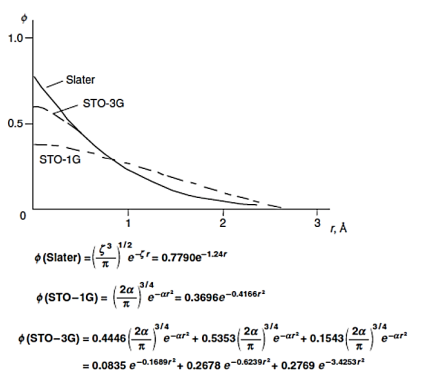
\includegraphics{fig/lzhx/微信图片_20211102165150}
\end{center}

\paragraph*{Contracted Gaussian type orbitals (CGTO's)}
\[\phi_{abc}^{CGTO}(x,y,z)=N\sum_{i=1}^n x^ay^bz^ce^{-\zeta r^2}\]
比较神奇的是,一般我们不叫这个基组CGTO,而是STO-nG。

下面给出的是STO-3G描述不同原子需要的函数个数,一般而言STO-3G都是作为计算体系的极小基:
\begin{center}
    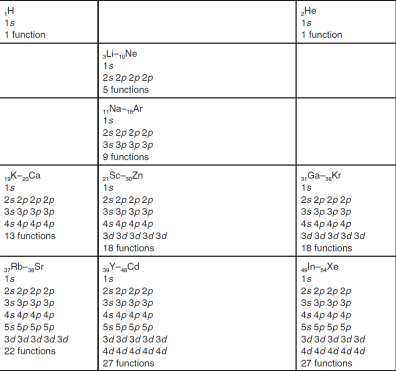
\includegraphics[scale=0.7]{fig/lzhx/微信图片_20211102171332.png}
\end{center}

\paragraph*{3–21G Split Valence and Double-Zeta Basis Set}
在这种基组下,我们把电子分为两种,核层(core orbitals)与价层(valence orbital),内层的轨道每一个轨道用一个包含三个Gaussian函数的基函数描述,价层每个轨道分为内层与外层,内层(inner shell)用两个Gaussian函数描述,外层(outer shell)用一个Gaussian函数描述,6-31G等同理:
\begin{center}
    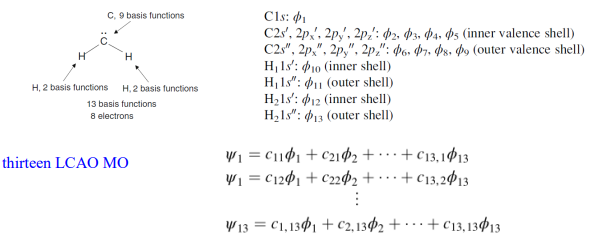
\includegraphics[scale=0.9]{fig/lzhx/微信图片_20211102172815}
\end{center}
\begin{center}
    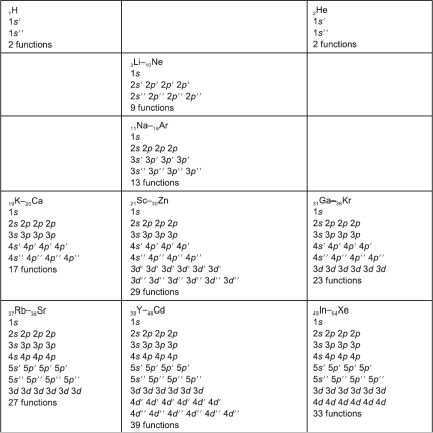
\includegraphics[scale=0.7]{fig/lzhx/微信图片_202111021728151}
\end{center}

\section{分子光谱}
在化学范围内,我们考虑一个分子的能量由平动、转动、振动、电子能量组成:
\[E=E_{tr}+E_{rot}+E_{vib}+E_{ele}\]
\begin{center}
    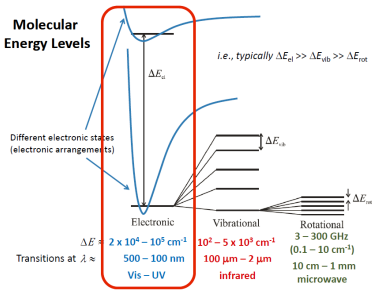
\includegraphics{fig/lzhx/微信图片_20211102175446.png}
\end{center}

与原子光谱类似,分子光谱也有类似的表达方式:
\[M^S\Lambda^{(+/-)}_\Omega\]

其中,$s$、$\Lambda$、$\Omega$由下式给出:
\[S=2s+1 \qquad \hat{J}_z\varPsi=\Lambda\varPsi \qquad \Omega=|\Lambda+S| \qquad \Lambda=\sum_ij_i \qquad S=\sum_iS_i\]

$\Lambda$的取值如下,判断的方法是看开壳层电子所在轨道的$j$值的矢量叠加:
\[\begin{array}{ll}
    \Lambda=0 & \Sigma \\
    \Lambda=\pm 1 & \Pi \\
    \Lambda=\pm 2 & \Delta \\
    \cdots
\end{array}\]

$\Omega$的结果通常用$g$或者$u$来表示,其取值可以通过判断$u$轨道上的单电子个数来判断——每一个在$u$上的电子其对称性都记为$u$,总的$\Omega$取值通过以下方式将各个$u$通过结合运算合成:
\begin{center}
    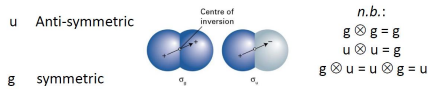
\includegraphics{fig/lzhx/微信图片_20211106011930.png}
\end{center}

分子谱相中右上角的角标$+/-$仅在$\Lambda$取值为$\Sigma$时显现,其取值由波函数轨道部分对称或反对称决定:对称时为+,反之为-。

$M$为按能量从低到高用符号$X$、$A$、$B$$\cdots$来表示,如:$X^3\Sigma^-_g$、$A^1\nabla^2_g$、$B^1\Sigma^+_g$。

谱相的多重度为:
\[
    \begin{array}{ll}
        2(2s+1) & if \quad \Lambda \neq 0 \\
        2s+1 & if \quad \Lambda = 0
    \end{array}
\]

\subsection{双原子分子光谱实例}
如果不考虑将电子激发到其他能级上,$O_2$分子可能的开壳层排布为:
\[
    \begin{array}{lcccccc}
        state & \pi_+(\alpha\beta)\pi_- & \pi_+(\alpha)\pi_-(\alpha) & \pi_+(\alpha)\pi_-(\beta) & \pi_+(\beta)\pi_-(\alpha) & \pi_+(\beta)\pi_-(\beta) & \pi_+\pi_-(\alpha\beta) \\
        M_L=  & 2 & 0 & 0 & 0 & 0 & -2 \\
        M_S=  & 0 & 1 & 0 & 0 & -1 & 0
    \end{array}
\]

当然,这么写是并不完全合理,由于全同性,对于对应相同谱相的电子组态我们无法区分,如1、6,3、4三对电子组态,因此,在正式确定对应于同一个谱相的电子组态时,我们需要按照波函数反对称化以及粒子全同性的要求将其两两线性组合。

如对1、6这组,首先写出其价层的$Slater$行列式,并定义简写:
\[
\varphi_1=\frac{1}{\sqrt{2}}
\begin{vmatrix}
    \pi_{g+}(1)\alpha(1) & \pi_{g+}(1)\beta(1) \\
    \pi_{g+}(2)\alpha(2) & \pi_{g+}(2)\beta(2)
\end{vmatrix}
:=
\begin{vmatrix}
    \pi_{g+}(1)\alpha(1) & \pi_{g+}(2)\beta(2)
\end{vmatrix}
\]
\[
\varphi_6=\frac{1}{\sqrt{2}}
\begin{vmatrix}
    \pi_{g-}(1)\alpha(1) & \pi_{g-}(1)\beta(1) \\
    \pi_{g-}(2)\alpha(2) & \pi_{g-}(2)\beta(2)
\end{vmatrix}
:=
\begin{vmatrix}
    \pi_{g-}(1)\alpha(1) & \pi_{g-}(2)\beta(2)
\end{vmatrix}
\]

由于我们指定了这两个电子排布在某个确定角动量的轨道上,这不符合粒子全同性的要求,当然更本质的原因是这两个波函数不是$\hat{S}^2$的本征函数,其自旋无意义,这里需要对两个态进行正交线性组合:
\[\Psi=\frac{1}{\sqrt{2}}(\varphi_1+\varphi_6) \qquad \Psi'=\frac{1}{\sqrt{2}}(\varphi_1-\varphi_6)\]

\[|M_L|=2 \qquad |M_S|=0 \qquad g \times g=g\]

故,这两组电子组态对应的分子谱项为:$^1\nabla^2_g$

同理,对2、5组:
\[
\varphi_2=\frac{1}{\sqrt{2}}
\begin{vmatrix}
    \pi_{g+}(1)\alpha(1) & \pi_{g-}(1)\alpha(1) \\
    \pi_{g+}(2)\alpha(2) & \pi_{g-}(2)\alpha(2)
\end{vmatrix}
=\frac{1}{\sqrt{2}}
\begin{vmatrix}
    \pi_{g+}(1) & \pi_{g-}(1) \\
    \pi_{g+}(2) & \pi_{g-}(2)
\end{vmatrix}
\alpha(1)\alpha(2)
\]
\[
\varphi_5=\frac{1}{\sqrt{2}}
\begin{vmatrix}
    \pi_{g+}(1)\beta(1) & \pi_{g-}(1)\beta(1) \\
    \pi_{g+}(2)\beta(2) & \pi_{g-}(2)\beta(2)
\end{vmatrix}
=\frac{1}{\sqrt{2}}
\begin{vmatrix}
    \pi_{g+}(1) & \pi_{g-}(1) \\
    \pi_{g+}(2) & \pi_{g-}(2)
\end{vmatrix}
\beta(1)\beta(2)
\]

这两种状态并不违反粒子全同性,故无需重新线性组合,他们对应相同的光谱项。
\[|M_L|=0 \qquad |M_S|=2 \qquad g \times g=g\]

由于轨道波函数部分反对称,故,这两组电子组态对应的分子谱项为:$^3\Sigma_g^-$

对3、4组:
\[
\varphi_3=\frac{1}{\sqrt{2}}
\begin{vmatrix}
    \pi_{g+}(1)\alpha(1) & \pi_{g-}(1)\alpha(1) \\
    \pi_{g+}(2)\beta(2) & \pi_{g-}(2)\beta(2)
\end{vmatrix}
=\frac{1}{\sqrt{2}}
\begin{vmatrix}
    \pi_{g+}(1) & \pi_{g-}(1) \\
    \pi_{g+}(2) & \pi_{g-}(2)
\end{vmatrix}
\alpha(1)\beta(2)
\]
\[
\varphi_4=\frac{1}{\sqrt{2}}
\begin{vmatrix}
    \pi_{g+}(1)\beta(1) & \pi_{g-}(1)\beta(1) \\
    \pi_{g+}(2)\alpha(2) & \pi_{g-}(2)\alpha(2)
\end{vmatrix}
=\frac{1}{\sqrt{2}}
\begin{vmatrix}
    \pi_{g+}(1) & \pi_{g-}(1) \\
    \pi_{g+}(2) & \pi_{g-}(2)
\end{vmatrix}
\beta(1)\alpha(2)
\]

显然,这样的排布不满足全同性的要求,重新线性组合得到:
\[\Psi=\frac{1}{2}(\pi_{g+}(1)\pi_{g-}(2)-\pi_{g-}(1)\pi_{g+}(2))(\alpha(1)\beta(2)+\beta(1)\alpha(2))\]
\[\Psi'=\frac{1}{2}(\pi_{g+}(1)\pi_{g-}(2)+\pi_{g-}(1)\pi_{g+}(2))(\alpha(1)\beta(2)-\beta(1)\alpha(2))\]
\[|M_L|=0 \qquad |M_S|=2 \qquad g \times g=g\]

考虑轨道部分,对$\Psi$,其最外层轨道部分反对称,故右上角表为-,同理$\Psi$右上角表为+,注意到$\Psi$的自选部分为三重态,故其左上角标为3而非单重态的1:
\[
    \begin{array}{ll}
        \Psi & ^3\Sigma_g^- \\
        \Psi' & ^1\Sigma_g^+ 
    \end{array}
\]

最后,按能量高低给氧分子的三个谱相表上相应符号:
\begin{center}
    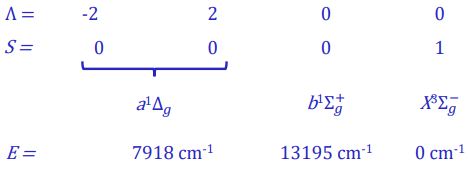
\includegraphics{fig/lzhx/微信图片_20211106140136.png}
\end{center}

\section{附录I:一点数学(微积分线代什么的自己去看书)}
\subsection{变量分离}
变量分离是解偏微分方程的常用方法,其核心是假设偏微分方程的解可以由几个以不同变量(组)为自变量的函数共同表示,即:
\[y(\bm{r}_1,\bm{r}_2,\cdot\cdot\cdot,\bm{r}_n)=y_1(\bm{r}_1)y_2(\bm{r}_2)\cdot\cdot\cdot y_n(\bm{r}_n)\]

这里,我们以含时薛定谔方程为例简要介绍一下变量分离,下列方程即为含时薛定谔方程:
\[i \hbar \frac{\partial \psi}{\partial t} =\hat{H}\psi:=\left (-\frac{\hbar^2}{2m}\nabla^2+V \right ) \psi\]

这里,我们假设解出的波函数$\psi(\bm{r},t)$可以被分成以下形式:
\[\psi(\bm{r},t)=\varPsi(\bm{r})\phi(t)\]

那么含时薛定谔方程可以改写成:

\[i \hbar \varphi \frac{\partial \phi}{\partial t}= -\frac{\hbar^2}{2m} \phi \nabla^2 \varPsi+V\varPsi\phi\]

显然,除了平凡解$\psi=0$外,我们可以认为解出的波函数仅在有限个点上取值为零,不考虑这些奇异点,我们将方程两边同时除以$\varphi$$\phi$:

\[i \hbar \frac{1}{\phi} \frac{\partial \phi}{\partial t}= -\frac{\hbar^2}{2m} \frac{1}{\varPsi} \nabla^2 \varPsi+V\]

显然我们可以给出一个能量单位的参数$E$使得原方程可以写成以下方程组:
\[\left\{
\begin{array}{r}
i\hbar\frac{1}{\phi}\frac{\partial\phi}{\partial t}=E\\
-\frac{\hbar^2}{2m}\frac{1}{\varPsi}\nabla^2\varPsi+V=E
\end{array} \right. \quad \Rightarrow \quad
\left\{
\begin{array}{l}
\phi(t)=\exp(-\frac{iEt}{\hbar})\\
\hat{H}\varPsi=E\varPsi
\end{array} \right.\]

\subsection{球坐标下的拉普拉斯算符展开}
球坐标与直角坐标的转换关系如下:
\[x=r\sin\theta\cos\phi, \quad y=r\sin\theta\cos\phi, \quad z=r\cos\theta\]
计算某个坐标下的梯度算子$\nabla$可以考虑对坐标向量$\bm{r}=(x,y,z)$求导并归一化得到。如球坐标的单位向量在直角坐标的基底下可以被表示为:
\begin{equation*}
\begin{aligned}
\hat{\bm{r}} &=\pdv{\bm{r}}{r}= (\sin\theta \cos\phi, \sin\theta \sin\phi, \cos\theta), \\
\hat{\bm{\theta}} &=\frac{1}{r}\pdv{\bm{r}}{\theta}= (\cos\theta \cos\phi, \cos\theta \sin\phi, -\sin\theta), \\
\hat{\bm{\phi}} &=\frac{1}{r\sin\theta}\pdv{\bm{r}}{\phi}= (-\sin\phi, \cos\phi, 0).
\end{aligned}
\end{equation*}
因此我们可以写出球坐标下的梯度算子$\nabla$:
\[\nabla=\hat{\bm{r}}\pdv{r}+\hat{\bm{\theta}}\frac{1}{r}\pdv{\theta}+\hat{\bm{\phi}}\frac{1}{r\sin\theta}\pdv{\phi}\]
当我们考虑计算球坐标下的拉普拉斯算子$\Delta=\nabla^2=\nabla\cdot\nabla$时,我们注意到球坐标的单位向量对坐标的导数并非简单的0或者1(在直角坐标系下的情况):
\begin{equation*}
\begin{aligned}
\frac{\partial \hat{\bm{r}}}{\partial r} &=\frac{\partial \hat{\bm{\theta}}}{\partial r}=\frac{\partial \hat{\bm{\phi}}}{\partial r}=0\\
\frac{\partial \hat{\bm{r}}}{\partial \theta} &= (\cos\theta \cos\phi, \cos\theta \sin\phi, -\sin\theta) = \hat{\bm{\theta}}, \\
\frac{\partial \hat{\bm{r}}}{\partial \phi} &= (-\sin\theta \sin\phi, \sin\theta \cos\phi, 0) = \sin\theta \, \hat{\bm{\phi}},\\
\frac{\partial \hat{\bm{\theta}}}{\partial \theta} &= (-\sin\theta \cos\phi, -\sin\theta \sin\phi, -\cos\theta) = -\hat{\bm{r}}, \\
\frac{\partial \hat{\bm{\theta}}}{\partial \phi} &= (-\cos\theta \sin\phi, \cos\theta \cos\phi, 0) = \cos\theta \, \hat{\bm{\phi}},\\
\frac{\partial \hat{\bm{\phi}}}{\partial \theta} &= (0, 0, 0) = \bm{0}, \\
\frac{\partial \hat{\bm{\phi}}}{\partial \phi} &= (-\cos\phi, -\sin\phi, 0) = -\sin\theta \, \hat{\bm{r}} - \cos\theta \, \hat{\bm{\theta}}.
\end{aligned}
\end{equation*}

因此在直角坐标系下的拉普拉斯算子$\nabla^2$可以表示成如下形式:
\[\nabla^2=(\bm{i}\frac{\partial}{\partial{x}}+\bm{j}\frac{\partial}{\partial{y}}+\bm{k}\frac{\partial}{\partial{z}}) \cdot (\bm{i}\frac{\partial}{\partial{x}}+\bm{j}\frac{\partial}{\partial{y}}+\bm{k}\frac{\partial}{\partial{z}})=\frac{\partial^2}{\partial{x}^2}+\frac{\partial^2}{\partial{y}^2}+\frac{\partial^2}{\partial{z}^2}\]
但我们并不能直接将球坐标系下的梯度做点乘得到球坐标下的拉普拉斯算子:
\[\nabla^2=(\hat{\bm{r}}\pdv{r}+\hat{\bm{\theta}}\frac{1}{r}\pdv{\theta}+\hat{\bm{\phi}}\frac{1}{r\sin\theta}\pdv{\phi}) \cdot (\hat{\bm{r}}\pdv{r}+\hat{\bm{\theta}}\frac{1}{r}\pdv{\theta}+\hat{\bm{\phi}}\frac{1}{r\sin\theta}\pdv{\phi}) \neq \frac{\partial^2}{\partial{r^2}}+\frac{1}{r^2}\frac{\partial^2}{\partial{\theta^2}}+\frac{1}{r^2sin^2 \theta }\frac{\partial^2}{\partial{\phi^2}}\]
需要对每一项分别计算,第一项:
\[
\hat{\mathbf{r}}\frac{\partial}{\partial r} \cdot \left(\hat{\mathbf{r}}\frac{\partial}{\partial r}\right) = \hat{\mathbf{r}} \cdot \left(\frac{\partial\hat{\mathbf{r}}}{\partial r}\frac{\partial}{\partial r} + \hat{\mathbf{r}}\frac{\partial^2}{\partial r^2}\right) = \hat{\mathbf{r}} \cdot \hat{\mathbf{r}}\frac{\partial^2}{\partial r^2} = \frac{\partial^2}{\partial r^2}
\]
第二项:
\[
\hat{\mathbf{r}}\frac{\partial}{\partial r} \cdot \left(\hat{\boldsymbol{\theta}}\frac{1}{r}\frac{\partial}{\partial \theta}\right) = \hat{\mathbf{r}} \cdot \left(\frac{\partial\hat{\boldsymbol{\theta}}}{\partial r}\frac{1}{r}\frac{\partial}{\partial \theta} + \hat{\boldsymbol{\theta}}\frac{\partial}{\partial r}\left(\frac{1}{r}\frac{\partial}{\partial \theta}\right)\right) = 0
\]
第三项:
\[
\hat{\mathbf{r}}\frac{\partial}{\partial r} \cdot \left(\hat{\boldsymbol{\phi}}\frac{1}{r\sin\theta}\frac{\partial}{\partial \phi}\right) = \hat{\mathbf{r}} \cdot \left(\frac{\partial\hat{\boldsymbol{\phi}}}{\partial r}\frac{1}{r\sin\theta}\frac{\partial}{\partial \phi} + \hat{\boldsymbol{\phi}}\frac{\partial}{\partial r}\left(\frac{1}{r\sin\theta}\frac{\partial}{\partial \phi}\right)\right) = 0
\]
第四项:
\[
\hat{\boldsymbol{\theta}}\frac{1}{r}\frac{\partial}{\partial \theta} \cdot \left(\hat{\mathbf{r}}\frac{\partial}{\partial r}\right) = \hat{\boldsymbol{\theta}} \cdot \left(\frac{\partial\hat{\mathbf{r}}}{\partial \theta}\frac{\partial}{\partial r} + \hat{\mathbf{r}}\frac{\partial^2}{\partial\theta\partial r}\right) = \hat{\boldsymbol{\theta}} \cdot \hat{\boldsymbol{\theta}}\frac{\partial}{\partial r} = \frac{1}{r}\frac{\partial}{\partial r}
\]
第五项:
\[
\hat{\boldsymbol{\theta}}\frac{1}{r}\frac{\partial}{\partial \theta} \cdot \left(\hat{\boldsymbol{\theta}}\frac{1}{r}\frac{\partial}{\partial \theta}\right) = \hat{\boldsymbol{\theta}} \cdot \left(\frac{\partial\hat{\boldsymbol{\theta}}}{\partial \theta}\frac{1}{r}\frac{\partial}{\partial \theta} + \hat{\boldsymbol{\theta}}\frac{1}{r}\frac{\partial^2}{\partial\theta^2}\right) = \hat{\boldsymbol{\theta}} \cdot \left(-\hat{\mathbf{r}}\frac{1}{r}\frac{\partial}{\partial \theta} + \hat{\boldsymbol{\theta}}\frac{1}{r}\frac{\partial^2}{\partial\theta^2}\right) = \frac{1}{r^2}\frac{\partial^2}{\partial\theta^2}
\]
第六项:
\[
\hat{\boldsymbol{\theta}}\frac{1}{r}\frac{\partial}{\partial \theta} \cdot \left(\hat{\boldsymbol{\phi}}\frac{1}{r\sin\theta}\frac{\partial}{\partial \phi}\right) = \hat{\boldsymbol{\theta}} \cdot \left(\frac{\partial\hat{\boldsymbol{\phi}}}{\partial \theta}\frac{1}{r\sin\theta}\frac{\partial}{\partial \phi} + \hat{\boldsymbol{\phi}}\frac{1}{r}\frac{\partial}{\partial \theta}\left(\frac{1}{r\sin\theta}\frac{\partial}{\partial \phi}\right)\right) = 0
\]
第七项:
\[
\hat{\boldsymbol{\phi}}\frac{1}{r\sin\theta}\frac{\partial}{\partial \phi} \cdot \left(\hat{\mathbf{r}}\frac{\partial}{\partial r}\right) = \hat{\boldsymbol{\phi}} \cdot \left(\frac{\partial\hat{\mathbf{r}}}{\partial \phi}\frac{\partial}{\partial r} + \hat{\mathbf{r}}\frac{\partial^2}{\partial\phi\partial r}\right) = \hat{\boldsymbol{\phi}} \cdot \left(\sin\theta\hat{\boldsymbol{\phi}}\frac{\partial}{\partial r}\right) = \frac{1}{r\sin\theta}\sin\theta\frac{\partial}{\partial r} = \frac{1}{r}\frac{\partial}{\partial r}
\]
第八项:
\[
\hat{\boldsymbol{\phi}}\frac{1}{r\sin\theta}\frac{\partial}{\partial \phi} \cdot \left(\hat{\boldsymbol{\theta}}\frac{1}{r}\frac{\partial}{\partial \theta}\right) = \hat{\boldsymbol{\phi}} \cdot \left(\frac{\partial\hat{\boldsymbol{\theta}}}{\partial \phi}\frac{1}{r}\frac{\partial}{\partial \theta} + \hat{\boldsymbol{\theta}}\frac{1}{r\sin\theta}\frac{\partial^2}{\partial\phi\partial\theta}\right) = \hat{\boldsymbol{\phi}} \cdot \left(\cos\theta\hat{\boldsymbol{\phi}}\frac{1}{r}\frac{\partial}{\partial \theta}\right) = \frac{1}{r\sin\theta}\cos\theta\frac{1}{r}\frac{\partial}{\partial \theta} = \frac{\cot\theta}{r^2}\frac{\partial}{\partial \theta}
\]
第九项:
\[\begin{aligned}
\hat{\boldsymbol{\phi}}\frac{1}{r\sin\theta}\frac{\partial}{\partial \phi} \cdot \left(\hat{\boldsymbol{\phi}}\frac{1}{r\sin\theta}\frac{\partial}{\partial \phi}\right) &= \hat{\boldsymbol{\phi}} \cdot \left(\frac{\partial\hat{\boldsymbol{\phi}}}{\partial \phi}\frac{1}{r\sin\theta}\frac{\partial}{\partial \phi} + \hat{\boldsymbol{\phi}}\frac{1}{r\sin\theta}\frac{\partial^2}{\partial\phi^2}\right)\\
&= \hat{\boldsymbol{\phi}} \cdot \left[(-\sin\theta\hat{\mathbf{r}} - \cos\theta\hat{\boldsymbol{\theta}})\frac{1}{r\sin\theta}\frac{\partial}{\partial \phi} + \hat{\boldsymbol{\phi}}\frac{1}{r\sin\theta}\frac{\partial^2}{\partial\phi^2}\right] = \frac{1}{r^2\sin^2\theta}\frac{\partial^2}{\partial\phi^2}
\end{aligned}
\]

将所有项合并并整理成标准形式:
\[
\nabla^2 = \frac{\partial^2}{\partial r^2} + \frac{2}{r}\frac{\partial}{\partial r} + \frac{1}{r^2}\frac{\partial^2}{\partial\theta^2} + \frac{\cot\theta}{r^2}\frac{\partial}{\partial\theta} + \frac{1}{r^2\sin^2\theta}\frac{\partial^2}{\partial\phi^2} = \frac{1}{r^2}\frac{\partial}{\partial r}\left(r^2\frac{\partial}{\partial r}\right) + \frac{1}{r^2\sin\theta}\frac{\partial}{\partial\theta}\left(\sin\theta\frac{\partial}{\partial\theta}\right) + \frac{1}{r^2\sin^2\theta}\frac{\partial^2}{\partial\phi^2}
\]

\section{附录II:氢原子薛定谔方程求解(级数解法)\label{hydrgen}}
利用分离变量法,我们假定定态波函数$\varPsi(r,\theta,\varphi)$可以表示成如下形式:
\[\varPsi(r,\theta,\varphi)=R(r)\Theta(\theta)\varPhi(\varphi)\]

带入定态薛定谔方程:
\[\hat{H}R(r)\Theta(\theta)\varPhi(\varphi)=ER(r)\Theta(\theta)\varPhi(\varphi)\]

将哈密顿算符展开,将拉普拉斯算符在极坐标系下展开,并整理方程,我们可以得到:
\[\frac{\Theta\varPhi}{r^2}\frac{\partial}{\partial{r}}(r^2\frac{\partial R}{\partial{r}})+\frac{R\varPhi}{r^2sin\theta}\frac{\partial}{\partial{\theta}}(sin\theta\frac{\partial \Theta}{\partial{\theta}})+\frac{R\Theta}{r^2sin^2 \theta }\frac{\partial^2 \varPhi}{\partial{\phi^2}}=-\frac{2m(E-V)}{\hbar^2}R\Theta\varPhi\]

在方程两边同时乘上因子$\frac{r^2sin^2 \theta}{R\Theta\varPhi}$,我们可以得到:
\[\frac{sin^2 \theta}{R}\frac{\partial}{\partial{r}}(r^2\frac{\partial R}{\partial{r}})+\frac{sin\theta}{\Theta}\frac{\partial}{\partial{\theta}}(sin\theta\frac{\partial \Theta}{\partial{\theta}})+\frac{1}{\varPhi}\frac{\partial^2 \varPhi}{\partial{\phi^2}}=-\frac{2m(E-V)}{\hbar^2}r^2sin^2 \theta\]

再通过移向,我们得到:
\[\frac{sin^2 \theta}{R}\frac{\partial}{\partial{r}}(r^2\frac{\partial R}{\partial{r}})+\frac{sin\theta}{\Theta}\frac{\partial}{\partial{\theta}}(sin\theta\frac{\partial \Theta}{\partial{\theta}})+\frac{2m(E-V)}{\hbar^2}r^2sin^2 \theta=-\frac{1}{\varPhi}\frac{\partial^2 \varPhi}{\partial{\phi^2}}\]

由于方程两边变量不同,若满足上述等式,方程左右两边都应等于同一个常数,不妨假设该常数为$m^2$,则我们可以得到两个方程:
\[\frac{\partial^2 \varPhi}{\partial{\phi^2}}+m^2\varPhi=0 \tag{a}\]
\[\frac{sin^2 \theta}{R}\frac{\partial}{\partial{r}}(r^2\frac{\partial R}{\partial{r}})+\frac{sin\theta}{\Theta}\frac{\partial}{\partial{\theta}}(sin\theta\frac{\partial \Theta}{\partial{\theta}})+\frac{2m(E-V)}{\hbar^2}r^2sin^2 \theta=m^2 \tag{4}\]

将方程$4$两边同时除以$sin^2 \theta$并整理,我们得到:
\[\frac{1}{R}\frac{\partial}{\partial{r}}(r^2\frac{\partial R}{\partial{r}})+\frac{2m(E-V)}{\hbar^2}r^2=\frac{m^2}{sin^2 \theta}-\frac{1}{\Theta sin\theta}\frac{\partial}{\partial{\theta}}(sin\theta\frac{\partial \Theta}{\partial{\theta}})\]

同样的,我们假定上述方程左右两边均等于参数$\beta$,于是我们又得到两个方程:
\[\frac{1}{R}\frac{\partial}{\partial{r}}(r^2\frac{\partial R}{\partial{r}})+\frac{2m(E-V)}{\hbar^2}r^2=\beta \tag{b}\]
\[\frac{m^2}{sin^2 \theta}-\frac{1}{\Theta sin\theta}\frac{\partial}{\partial{\theta}}(sin\theta\frac{\partial \Theta}{\partial{\theta}})=\beta \tag{c}\]

至此,我们将定态薛定谔方程拆分成三个含不同变量的常微分方程$a,b,c$。
\subsection{Φ方程的求解}
由球坐标中$\varphi$的范围及其边界条件$\varPhi(x)=\varPhi(x+2\pi)$、归一化条件以及方程$a$,我们在这一小节将要处理的对象是柯西问题:
\[\frac{\mathrm{d}^2 \varPhi}{\mathrm{d}{\phi^2}}+ m^2 \varPhi=0 \qquad \varPhi(x)=\varPhi(x+2\pi) ,\int_{0}^{2\pi}\varPhi^{*}\varPhi d\phi=1\]

方程$a$的通解形式为:
\[\varPhi(\phi)=C_1 e^{im\phi}+C_2 e^{-im\phi}\]

带入上述边界条件,我们得到上述柯西问题的解:
\[\varPhi(\phi)=\frac{1}{\sqrt{2\pi}}e^{im\phi} \qquad (m=0,\pm 1,\pm 2\cdot\cdot\cdot)\]

但显然,上述解与方程$a$的通解并不相同。但问题不大,由于微分方程特解的线性叠加性,我们可以选取一对绝对值为$|m|$的解线性叠加成我们认知中的方程$a$的通解。

\subsection{Θ方程的求解}
对方程$c$,我们做以下代换:
\[x=cos\theta \qquad \frac{\mathrm{d} \Theta}{\mathrm{d} x}=\frac{\mathrm{d} \Theta}{\mathrm{d} \theta}\left ( \frac{\mathrm{d} x}{\mathrm{d} \theta} \right )^{-1}=-\frac{1}{sin\theta} \frac{\mathrm{d} \Theta}{\mathrm{d} \theta} \qquad y(x)=\Theta(\theta)\]

则方程$c$可以改写成以下形式:
\[\frac{m^2}{1-x^2}-\frac{1}{y}\frac{\mathrm{d}}{\mathrm{d}{x}} \left [(1-x^2) \frac{\mathrm{d} y}{\mathrm{d}{x}} \right ]=\beta\]

经整理,我们可以将上述方程改写成:
\[\frac{\mathrm{d}}{\mathrm{d}{x}} \left [(1-x^2) \frac{\mathrm{d} y}{\mathrm{d}{x}} \right ]+\left (\beta- \frac{m^2}{1-x^2} \right )y=0\]

上述方程即为连带$Legendre$方程。

为了求解上述方程,我们需要从其简化入手,下面我们将给出连带$Legendre$方程的简化,$Legendre$方程:
\[\frac{\mathrm{d}}{\mathrm{d}{x}} \left [(1-x^2) \frac{\mathrm{d} y}{\mathrm{d}{x}} \right ]+\beta y=0\]

我们将用级数解法求解该方程,为了保证级数解法的正确性,我们引用一下定理保证在我们给定条件下的$Legendre$方程的解存在且唯一:

\textbf{定理} \qquad 如果$p(z)$和$q(z)$在圆$|z-z_0|<R$内单值解析,则在此圆内二阶线性微分方程的初值问题:
\[\frac{\mathrm{d}^2w}{\mathrm{d}x^2}+p(z)\frac{\mathrm{d}w}{\mathrm{d}x}+q(z)w=0\]
\[w(z_0)=a \qquad w^{'}(z_0)=b \qquad (\forall a,b \in \mathbb{C})\]
的解存在且唯一,并且解$w(z)$在这个圆内单值解析。

下面我们将开始求解$Legendre$方程,其中自变量$x$定义在$[-1,1] \subset \mathbb{R}$,我们首先取$x_0=0$,显然0是$Legendre$方程的常点,因此,我们假设方程的解在$x_0=0$的邻域内可以展开成一下形式:
\[y=\sum_{k=0}^{+\infty}c_kx^k\]

将展开式带入$Legendre$方程,并整理,我们得到:
\[\sum_{k=0}^{+\infty} \left \{ (k+2)(k+1)c_{k+2}-[k(k+1)-\beta]c_k \right \}x^k=0\]

然后我们得到了递推关系:
\[c_{k+2}=\frac{k(k+1)-\beta}{(k+2)(k+1)}c_k\]

进而:
\[c_{2k}=\prod_{n=1}^{k}\frac{(2k-1)(2k-2)-\beta}{(2k)(2k-1)}c_0\]
\[c_{2k+1}=\prod_{n=1}^{k}\frac{(2k)(2k-1)-\beta}{(2k)(2k+1)}c_1\]

因此,我们可以将方程的解按奇偶项拆开:
\[y(x)=c_1y_0(x)+c_2y_1(x)\]
\[y_0(x)=1+\sum_{k=1}^{+\infty}\frac{c_{2k}}{c_0}x^{2k}\]
\[y_1(x)=x+\sum_{k=1}^{+\infty}\frac{c_{2k+1}}{c_1}x^{2k+1}\]

容易看出当x取值$x= \pm 1$时,无穷级数$y_0(x)$、$y_1(x)$发散,与边界条件$|y(\pm 1)|< +\infty$矛盾,为了解决这个问题,我们将要使得无穷级数$y_0(x)$、$y_1(x)$退化为有限项,为此,我们将对特征值$\lambda$赋值:
\[\beta=l(l+1) \qquad l \in \mathbb{N}_{+}\]
\[y_0(x)=\sum_{k=0}^{+\infty}\frac{2^{2k}}{(2k)!}\frac{\Gamma(k-\frac{l}{2})\Gamma(\frac{l+1}{2}+k)}{\Gamma(-\frac{l}{2})\Gamma(\frac{l+1}{2})}x^{2k}\]
\[y_0(x)=\sum_{k=0}^{+\infty}\frac{2^{2k}}{(2k+1)!}\frac{\Gamma(k-\frac{l-1}{2})\Gamma(\frac{l}{2}+1+k)}{\Gamma(-\frac{l-1}{2})\Gamma(\frac{l}{2}+1)}x^{2k+1}\]

此时,无穷级数$y(x)$退化成2l项的有限级数$P_l(x)$,我们得到了该方程的本征函数解,也即$Legendre$多项式,在定义域内收敛:
\[P_l(x)=\sum_{k=0}^{[l/2]}(-1)^k \frac{(2l-2k)!}{2^l k! (l-k)!(l-2k)!}x^{l-2k}\]

回到连带$Legendre$方程,我们容易求出方程在$x= \pm 1$与$x=\infty$的指标为$\rho= \pm \frac{m}{2}$,于是我们做以下代换:
\[y=(x^2-1)^{\frac{m}{2}}v(x)\]

带入连带$Legendre$方程展开整理得:
\[(1-x^2)v^{''}-2(m+1)xv^{'}+[\beta-m(m+1)]v=0 \tag{d}\]

如果我们对$Legendre$方程求m次导:
\[\frac{\mathrm{d^{m+1}}}{\mathrm{d}{x^{m+1}}} \left [(1-x^2) \frac{\mathrm{d} y}{\mathrm{d}{x}} \right ]+\beta y^{(m)}=0\]
\[(1-x^2)\frac{\mathrm{d^{m+2}}y}{\mathrm{d}{x^{m+2}}}-2(m+1)x\frac{\mathrm{d^{m+1}}y}{\mathrm{d}{x^{m+1}}}+[\beta-m(m+1)]\frac{\mathrm{d^{m}}y}{\mathrm{d}{x^{m}}}=0\]

发现其与方程d形式相同。

于是,我们能直接写出连带$Legendre$方程的解:
\[y=(x^2-1)^{\frac{m}{2}}\frac{\mathrm{d^{m}}P_l(x)}{\mathrm{d}{x^{m}}}=(x^2-1)^{\frac{m}{2}}\frac{\mathrm{d^{m}}}{\mathrm{d}{x^{m}}}\sum_{k=0}^{[l/2]}(-1)^k \frac{(2l-2k)!}{2^l k! (l-k)!(l-2k)!}x^{l-2k}:=(x^2-1)^{\frac{m}{2}}P^m_l(x)\]

至此,方程b的解可以写成:
\[\Theta(\theta)=(-1)^msin^m(\theta)P^m_l(cos\theta)\]

同时为了满足归一化条件e,$\Theta(\theta)$最终可以表示成:
\[\int_0^{\pi}\Theta_{l,m}^{*}(\theta)\Theta_{l^{'},m^{'}}(\theta)sin\theta d\theta=\nabla^2_{l,l^{'}} \cdot \nabla^2_{m,m^{'}} \tag{e}\]
\[\Theta_{l,m}(\theta)=\sqrt{\frac{(2l-1)(l-|m|)!}{2(l+|m|)!}}P^{m}_l(cos\theta) \qquad |m| \leqslant l\]

此外,$Legendre$多项式也可以通过$Rodrigue$公式定义:
\[P_l(x) \equiv \frac{1}{2^ll!} \left ( \frac{\mathrm{d}}{\mathrm{d}x} \right )^l(x^2-1)^l\]

\textbf{补充说明:本小节涉及到的$m$为加说明均取绝对值。}

\subsection{R方程的求解}

对方程b,我们要处理的是以下柯西问题:
\[\frac{1}{R}\frac{\partial}{\partial{r}}(r^2\frac{\partial R}{\partial{r}})+\frac{2m(E-V)}{\hbar^2}r^2=\beta \qquad r>0 \qquad V=-\frac{e}{4 \pi \varepsilon_0 r}\]

对上述柯西问题,我们做以下代换并整理可以得到方程:
\[u \equiv rR\]
\[-\frac{\hbar^2}{2m}\frac{\mathrm{d^2}u}{\mathrm{d}r^2}+ \left (\frac{\hbar^2}{2m}\frac{l(l+1)}{r^2}-\frac{e}{4 \pi \varepsilon_0r} \right )u=Eu\]

容易看出,当$r \rightarrow +\infty$时,
\[u=Ae^{-\frac{\sqrt{-2mE}}{\hbar}r}+Be^{\frac{\sqrt{-2mE}}{\hbar}r}\]

当$E>0$时,容易看出u不收敛于0,为非束缚态;当$E<0$时,我们可以取$B=0$使得当$r \rightarrow +\infty$时$u \rightarrow 0$,因此,我们取$E<0$。

继续通过代换简化方程形式:
\[\kappa \equiv \frac{\sqrt{-2mE}}{\hbar} \qquad \rho \equiv \kappa r \qquad \rho_o \equiv \frac{me^2}{2 \pi \varepsilon_0 \hbar^2 \kappa}\]
\[\frac{\mathrm{d^2}u}{\mathrm{d}\rho^2}=\left [ 1-\frac{\rho_0}{\rho}+\frac{l(l+1)}{\rho^2} \right ]u\]

当$\rho \rightarrow +\infty$,原方程近似为:
\[\frac{\mathrm{d^2}u}{\mathrm{d}\rho^2}=u\]

其解为:
\[u(\rho)=Ae^{-\rho}+Be^{\rho}\]

由$\lim_{\rho \rightarrow +\infty}u(\rho)=0$,得到$B=0$,最终解应近似为:
\[u(\rho) \sim Ae^{-\rho}\]

当$\rho \rightarrow 0$,原方程近似为:
\[\frac{\mathrm{d^2}u}{\mathrm{d}\rho^2}=\frac{l(l+1)}{\rho^2}u\]

可以验证其解为:
\[u(\rho)=C\rho^{l+1}+D\rho^{-l}\]

由$\lim_{\rho \rightarrow 0}u(\rho)=0$,得到$D=0$,最终解应近似为:
\[u(\rho) \sim C\rho^{l+1}\]

由于$\rho \rightarrow +\infty$与$\rho \rightarrow 0$均在定义域范围内。所以最终$u(\rho)$的解应包含上述的两个部分,不妨假设$u(\rho)$为以下形式:
\[u(\rho)=\rho^{l+1}e^{-\rho}v(\rho)\]

于是,原方程可以展开为:
\[\rho\frac{\mathrm{d^2}v}{\mathrm{d}\rho^2} +2(l+1-\rho)\frac{\mathrm{d}v}{\mathrm{d}\rho}+[\rho_0-2(l+1)]v=0 \]

假定$v(\rho)$可以展开成如下泰勒级数:
\[v(\rho)=\sum_{j=0}^{+\infty}c_j\rho^j\]

则原方程可以展开成:
\[\sum_{j=0}^{+\infty}j(j+1)c_{j+1}\rho^j+2(l+1)\sum_{j=0}^{+\infty}(j+1)c_{j+1}\rho^j-2\sum_{j=0}^{+\infty}jc_j\rho^j+[\rho_0-2(l+1)]\sum_{j=0}^{+\infty}c_j\rho^j=0\]

由于$\rho$取值的任意性,上述方程同阶项系数和应为0,即:
\[j(j+1)c_{j+1}+2(l+1)(j+1)c_{j+1}-2jc_j+[\rho_0-2(l+1)]c_j=0\]

整理得到:
\[c_{j+1}=\frac{2(l+1+j)-\rho_0}{(j+1)(j+2l+2)}c_j\]

对上述递推关系做估计,当$j \rightarrow +\infty$,有:
\[c_{j+1}=\frac{2(l+1+j)-\rho_0}{(j+1)(j+2l+2)}c_j \sim \frac{2j}{(j+1)j}c_j=\frac{2}{(j+1)}c_j\]

那么我们将可以得到:
\[c_j \sim \frac{2^j}{j!}c_0\]
\[v(\rho) \sim c_0\sum_{j=0}^{+\infty}\frac{2^j}{j!}\rho^j=c_0e^{2\rho}\]
\[u(\rho) \sim c_0\rho^{l+1}e^{\rho}\]

可以看出,当$v(\rho)$3为无穷级数时,$u(\rho)$发散,为了解决这个问题,我们可以同样利用上一小节的思路,将无穷级数截断使之退化成有限项级数,保证其收敛性,因此必然存在一个$j_{max}$使得:
\[c_{j_{max}+1}=\frac{2(l+1+j_{max})-\rho_0}{(j_{max}+1)(j_{max}+2l+2)}c_{j_{max}}=0\]

即:
\[2(l+1+j_{max})-\rho_0=0\]

这时,我们定义:
\[n \equiv l+1+j_{max}\]

此时,无穷级数$v(\rho)$退化成了$n-l$项的有限项级数:
\[v(\rho)=L_{n-l-1}^{2l+1}(2\rho)\]

其中$L_q(x)$为$Laguerre$多项式,$L_{q-p}^{p}(x)$为连带$Laguerre$多项式:
\[L_{q-p}^{p}(x)=(-1)^p \left ( \frac{\mathrm{d}}{\mathrm{d}x} \right )^qL_q(x)\]\
\[L_q(x)=e^x\left ( \frac{\mathrm{d}}{\mathrm{d}x} \right )^q(e^{-x}x^q)\]

这里的n也就是主量子数,从其定义式上我们可以很明显得看出角量子数的取值应为:
\[l=0,1,2, \cdot\cdot\cdot ,n-1\]

我们也能看出:
\[\rho_0=2n\]

再结合$\rho_0$与$\kappa$的定义式,我们可以得到:
\[E_n=- \left [\frac{m}{2\hbar^2} \left ( \frac{e^2}{4 \pi \varepsilon_0} \right )^2 \right ] \frac{1}{n^2}\]

以及玻尔半径$a$:
\[\frac{4 \pi \varepsilon_0 \hbar^2}{me^2}=0.529 \times 10^{-10}m\]

最终,再根据归一化条件,我们可以写出方程b的解$R(r)$:
\[R(r)=\sqrt{ \left (\frac{2}{na} \right )^3 \frac{(n-l-1)!}{2n[(n+l)!]^3}}e^{-\frac{r}{na}}\left (\frac{2r}{na} \right )^l \left [L_{n-l-1}^{2l+1} \left ( \frac{2r}{na} \right ) \right ]\]

至此,上述通过分离变量得到的三个方程全部解出。

\subsection{小结}
汇总一下上述三个方程的解:
\[R_{n,l}(r)=\sqrt{ \left (\frac{2}{na} \right )^3 \frac{(n-l-1)!}{2n[(n+l)!]^3}}e^{-\frac{r}{na}}\left (\frac{2r}{na} \right )^l \left [L_{n-l-1}^{2l+1} \left ( \frac{2r}{na} \right ) \right ]\]
\[\Theta_{l,m}(\theta)=\sqrt{\frac{(2l-1)(l-|m|)!}{2(l+|m|)!}}P^{m}_l(cos\theta)\]
\[\varPhi_{m}(\phi)=\frac{1}{\sqrt{2\pi}}e^{im\phi}\]

两个角度变量函数还能合并为$Y_l^m(\theta,\phi)$:
\[Y_l^m(\theta,\phi)=\varepsilon \sqrt{\frac{(2l-1)(l-|m|)!}{4 \pi (l+|m|)!}}e^{im\phi}P^{m}_l(cos\theta)\]

其中,当$m \geq 0$时$\varepsilon=(-1)^m$,当$m \leq 0$时$\varepsilon=1$,以满足其自动正交性。

因此,氢原子定态波函数的解$\varPsi_{n,l,m}$为:
\[\varPsi_{n,l,m}=\sqrt{ \left (\frac{2}{na} \right )^3 \frac{(n-l-1)!}{2n[(n+l)!]^3}}e^{-\frac{r}{na}}\left (\frac{2r}{na} \right )^l \left [L_{n-l-1}^{2l+1} \left ( \frac{2r}{na} \right ) \right ]Y_l^m(\theta,\phi)\]
\chapter{核磁初步}
\section{一维核磁}
\subsection{磁自旋动量、磁矩和磁矩的能量}

在非相对论量子力学框架下,自旋的行为是通过类比角动量的行为来定义的(在学到了量子力学里可以推导),磁自旋动量$M_s$与自旋量子数$S$之间的关系(当考虑电子自旋时,自旋量子数为单电子数$n$的$\frac{1}{2}$):
\[\hat{J}^2 \varPsi = M_l^2 \varPsi \qquad M_s=\sqrt{l(l+1)} \hbar \qquad\]
\[\hat{S}^2 \varPsi = M_s^2 \varPsi \qquad M_s=\sqrt{S(S+1)} \hbar \qquad\]

磁自旋动量是一个高维向量,我们并不方便直接去研究其性质,但是我们可以在$\mathbb{R}^3$空间中研究其投影$m_{s_z}$,我们知道磁自旋动量的投影是空间量子化的,每个自旋量子数对应一不同磁自旋动量在空间上的量子化投影,共计$2S+1$个:
\[\hat{S_z} \varPsi =m_s \hbar \varPsi \qquad M_{s_z}:=m_s \hbar \qquad (m_s=-S,-S+1,...,S-1,S)\]

经典力学中带电的旋转体具有磁矩,这点在量子力学中直接被沿用,粒子自旋的磁矩$\mu$平行且正比于自旋角动量$M_{s_z}$,比例系数为磁旋比$\gamma$,这里给出磁矩和磁自旋动量的关系式:
\[\mu=\gamma M_s=\gamma \sqrt{S(S+1)} \hbar= g_N \sqrt{S(S+1)}  \mu_N\]

我们这里统一规定磁场方向为z轴正向,磁矩的同样也是一个高维向量,其投影同样也是空间量子化的,因此我们对磁矩$\mu$做$\mathbb{R}^3$空间的投影:
\[\mu_z=\gamma M_{s_z}=\gamma m_s \hbar \qquad (m_s=-S,-S+1,...,S-1,S)\]

则磁矩在磁场中的势能可以写成:
\[E=-\mu \cdot B_0=-\mu_zB_0=-\gamma m_s \hbar B_0 \qquad  (m_s=-S,-S+1,...,S-1,S)\]

由于核自旋能级跃迁的选律为$\Delta m= \pm 1$,以氢核为例,其$m_s= \pm \frac{1}{2}$,则使其跃迁即发生核磁共振现象的光子频率应为:
\[\nu_0 = \frac{\Delta E}{h}=\frac{\gamma \hbar B_0}{h}=\frac{\gamma B_0}{2\pi} \tag{a}\]

\begin{center}
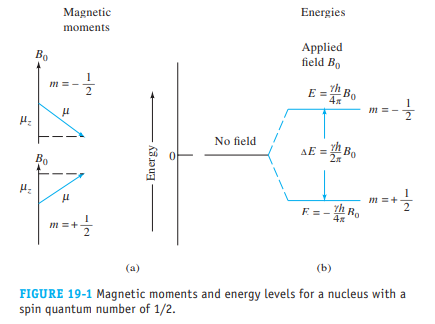
\includegraphics[scale=0.8]{./fig/hc/hc1.png}
\end{center}

\subsection{磁场下的核自旋能级}

核磁得到的数据是一组多次长时间(相对于瞬时而言)累计的信号,因此不同核自旋能级上的离子分部大致满足玻尔兹曼分布:
\[\rho_i=\frac{e^{-\frac{E_i}{kT}}}{Q} \qquad Q=\sum_{i=1}^{2S+1}e^{-\frac{E_i}{kT}} \tag{b}\]

由玻尔兹曼分布可知,与$B_0$同向的核自旋动量对应的进动圆锥面上分布这更多的粒子,不同核自旋动量对应的进动圆锥面上分布着不同数目的粒子。

\subsection{化学位移}

根据(a)式,我们可以关联起磁场与核自旋能差,但实际上,因为原子核并不会单独存在以及原子核并不是在任何情况下均不会发生变化的,分子中的电子云以及少量核自身的变化会产生一个与外加场相反的磁场抵消一部分外加场,使得\textbf{原子核感受到的磁场}并非完整的外加场,所以我们也可以定义一个屏蔽常数$\sigma$来描述这种屏蔽效应:
\[\nu =\frac{\gamma B_e}{2\pi}=\frac{\gamma (B_0-B')}{2\pi}:=\frac{\gamma B_0}{2\pi}(1-\sigma) \]

根据化学位移的定义我们可以有:
\[\delta=\frac{\nu_r-\nu_s}{\nu_s} \times 10^6=\frac{B_r-B_s}{B_s} \times 10^6=\frac{\sigma_s-\sigma_r}{1-\sigma_s} \times 10^6\]

\subsection{宏观磁矩、拉莫尔方程、核磁共振原理}

\textbf{核磁共振是一个大量分子的行为},那么我们可以知道,对于不同分子对应相同磁量子数的磁矩在空间上的分布应该是均匀的,如果我们把这些磁矩包起来,我们可以得到一个圆锥面,我们将这个圆锥面称之为进动圆锥面,采用这个命名这也许比较显然,因为原子核磁自旋轴向与磁矩重合,因此歪掉的磁矩在磁场会使得原子核发生进动。

由玻尔兹曼分布我们知道,粒子在不同进动圆锥面分布不均,因此,我们定义一个宏观磁矩M,其等于单位体积内所有粒子的磁矩的矢量和:
\[\overrightarrow{M}=\sum_i \overrightarrow{\mu}\]

定义单位体积磁矩而非整体磁矩主要的考虑是,为保证核磁能源源不断产生信号,粒子核自旋分布必须时刻保持近玻尔兹曼分布,即朝上的自旋始终多于朝下的自旋,因此整体核自旋方向应保持近平行于z轴,所以我们选取给出信号后被激发的部分或者所有粒子为一个整体做为对象。

对其进行正交分解得到沿着磁场方向的矢量和垂直磁场方向的矢量:
\[\overrightarrow{M}=\overrightarrow{M_{par}}+\overrightarrow{M_{prep}} \]

当无外加信号场时,$\overrightarrow{M_{perp}} \approx 0$,此时认为仅有沿磁场方向的$\overrightarrow{M_{par}}$,显然$\overrightarrow{M_{par}}>0$,记此时的$\overrightarrow{M_{par}}$为$\overrightarrow{M_0}$。

当未发生核磁共振的时候,在外加场的作用下,核自旋运动会产生核的进动(联想歪掉的陀螺),核自旋轴(单个核磁矩)进动围绕着z轴(磁力线),其进动的角速度和磁场有以下关系(虽然线性外加场下单个磁矩是歪的,但宏观磁矩依然是沿z轴正方向的):
\[\omega=\gamma B \tag{c}\]

此关系成为拉莫尔方程,这种进动也称之为拉莫尔进动。所谓核磁共振也就是\textbf{外加场在与某种拉莫尔进动同频的情况下为该拉莫尔进动提供能量}。下面我们来证明这个方程:

简单证明:

在外加场$B_0$存在时,核自旋进动的频率为:
\[\nu = \frac{\gamma B}{2 \pi}\]

故进动的角速度为:
\[\omega = 2 \pi \nu =2 \pi \cdot \frac{\gamma B}{2 \pi}= \gamma B\]

或者我们可以再严谨一点:

在均匀磁场$B$中,每单位体积磁矩所受力矩$M$为:

\[M=\mu \times B\]

于是根据角动量定理,得:

\[\frac{\mathrm{dL}}{\mathrm{d}t}=-M=-\mu \times B=-\gamma L \times B=\omega \times L\]

故:

\[\omega=-\gamma B\]

更进一步,我们甚至还能算出磁旋比$\gamma$,假定样品质点比荷都是$e/m$,把物体划分为许多体积元$d\tau$,则每个体积元的质量与电荷可表示为$de=\frac{e}{m}dm$,以$v$表示该体积元的速度,则电流密度$j$可表示为$j=v\frac{e}{m}\frac{dm}{d\tau}$,于是磁矩:

\[\mu=\frac{1}{2}\int r \times j d\tau=\frac{1}{2}\int r \times v\frac{e}{m}\frac{dm}{d\tau} d\tau=\frac{1}{2}\int r \times v\frac{e}{m}dm=\frac{e}{2m}\int r \times v dm=\frac{e}{2m}L\]

故磁旋比$\gamma$:

\[\gamma=\frac{e}{2m}\]

\begin{center}
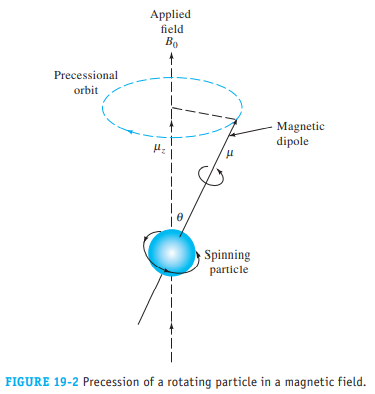
\includegraphics[scale=0.6]{./fig/hc/hc2.png}
\end{center}

拉莫尔方程告诉我们,带电体(这里是核自旋)在外磁场的存在下会绕外磁场进动,自然而然,我们可以知道宏观磁矩也会绕外磁场进动,在不发生核磁共振时外加场与宏观磁矩重合,可以认为宏观磁矩“零距离”绕磁场进动,这件事意味着我们只需要讨论磁场的取向就能较好地表述核磁共振。

这里给个例子,我们在三维直角坐标系里xOy平面上给定两个单位圆并记其上的一条半径分别为a、b,标记半径为a的圆以角速度$\omega$顺时针转动,标记半径为b的圆也以角速度$\omega$逆时针转动,两圆均以速度$v$朝z轴正方向运动,刚开始时a、b均与x轴正半轴重合。设半径a、b与圆周交点分别为A$(x_1,y_1,vt)$、B$(x_2,y_2,vt)$,可以写出A、B两点带时间参数的坐标:
\[A=(cos(\omega t),-sin(\omega t),vt) \qquad B=(cos(\omega t),sin(\omega t),vt)\]

考虑A、B中点O,则可以写出O点带时间参数的坐标:
\[O=(cos(\omega t),0,vt)\]

这时,我们会发现O点在曲线$x=cos(\frac{\omega z}{v})$上运动,这意味着我们用两个运动速度相同方向相反的圆偏振合成出了交变线偏振,当然同样的我们也可以将线性交变线偏振拆成两个方向相反的圆偏振。

因为磁场也是一种电磁波,有了上面的例子,我们可以知道:给原子核加上一个线偏振磁场相当于给原子核加上两个角速度方向相反、大小与某磁自旋量子数对应进动相同、垂直于原外加场的圆偏振磁场:
\[\overrightarrow{B}=\overrightarrow{B_0}+\overrightarrow{B'}=\overrightarrow{B_0}+\overrightarrow{B_{perp}}+\overrightarrow{-B_{perp}}\]

因为与进动方向相反的圆偏振磁场与进动在时域上正交,所有其对宏观磁矩的进动是没有贡献的,因此,我们可以给出对宏观磁矩的有效磁场$B_e$:
\[\overrightarrow{B_e}=\overrightarrow{B_0}+\overrightarrow{B_{perp}}\]

在实验室坐标系O-xyz下,宏观磁矩在旋转,磁场$\overrightarrow{B_{perp}}$也在旋转,当然我们也可以选定一个绕z轴旋转的坐标系固定磁场和宏观磁矩。所以在旋转坐标系O-x'y'z'中对宏观磁矩的有效磁场$B_e$在该坐标系下表达式为:
\[\overrightarrow{B_e}=\overrightarrow{B_0}+\overrightarrow{B_{perp}}+\overrightarrow{\frac{\omega}{\gamma}} \tag{d}\]

在旋转坐标系O-x'y'z'中$\overrightarrow{B_{perp}}$是固定的,便于处理,这也是为什么我们选择旋转坐标系的原因,这里,我们不妨将$\overrightarrow{B_{perp}}$固定在x'轴正方向。

共振时$\omega=\omega_0=2\pi \nu_0 \ , \ \overrightarrow{B_0}+\overrightarrow{\frac{\omega}{\gamma}}=0$,则有:
\[\overrightarrow{B_e}=\overrightarrow{B_{perp}} \tag{e}\]

不共振时,我们也能改写上式为:
\[\overrightarrow{B_e}=\overrightarrow{B_0}+\overrightarrow{\frac{\omega}{\gamma}}+\overrightarrow{B_{perp}}=\overrightarrow{\frac{\omega_0+\omega}{\gamma}}+\overrightarrow{B_{perp}}\]

其中$\omega_0$与$B_0$同向,$\omega$与$B_0$反向。

根据上面的讨论,我们知道,当发生核磁共振时,在旋转坐标系O-x'y'z'中,宏观磁矩$M$绕着x'轴转动,也就是发生从z'轴正方向到y'轴的偏转,其垂直外加场$B_0$的分量$M_{perp} \neq 0$,当撤去外加场$B'$,歪掉的宏观磁矩$M$会通过弛豫过程回复到原先方向。在实验室坐标系O-xyz下,在这个回复的过程中宏观磁矩$M$依旧在旋转,依然会继续切割外加场$B_0$产生信号直至其垂直外加场$B_0$的分量$M_{perp}=0$。通过检测弛豫信号,我们可以去推断这个原子核的自旋情况及其外部电子云的分布,当然对这个时域上的弛豫信号我们可以对其傅里叶变换研究其频域谱,这也就是我们常见的一维谱。

\subsection{弛豫过程}

我们都知道每一张核磁谱都是多次信号累加平均后得到的,这就意味着每次激发后激发态的原子需要回复到基态,我们把恢复到基态的这个过程称之为弛豫(relaxation)。从直观上来说,弛豫过程就是将倾斜的宏观磁矩扶正,我们有两个过程实现这个过程:

\qquad 1、将$M_{par}$的数值回复到$M_0$;

\qquad 2、将$M_{perp}$的数值减小至0;

第一种过程称为纵向弛豫,又称自旋-晶格耦合(spin-lattice relaxation),这里的晶格指的是环境,第二种过程称为横向弛豫。

对于纵向弛豫,核磁共振时,宏观矢量$\overrightarrow{M}$倾倒,$B_e$沿外加场分量变小,核自旋跃迁的能隙也变小,由于激发未饱和,基态的分子数多与激发态的分子数,能隙的变小意味着分子从磁场中吸收能量,这与核磁共振现象的描述是自洽的。纵向弛豫这是上述过程的逆过程——宏观矢量$\overrightarrow{M}$回正,$B_e$沿外加场分量变大,核自旋跃迁的能隙也变大,分子向磁场中释放能量。

对于横向弛豫,核磁共振的激发使得宏观矢量分量$\overrightarrow{M_{perp}}$不再为0,在横向上磁场分布不再均匀,这时,分子通过横向弛豫回复宏观矢量的过程是熵驱动的,分子本身不均匀的磁矩也有一定的贡献。

一般来说,纵向弛豫的耗时会大于等于横向弛豫。

\begin{center}
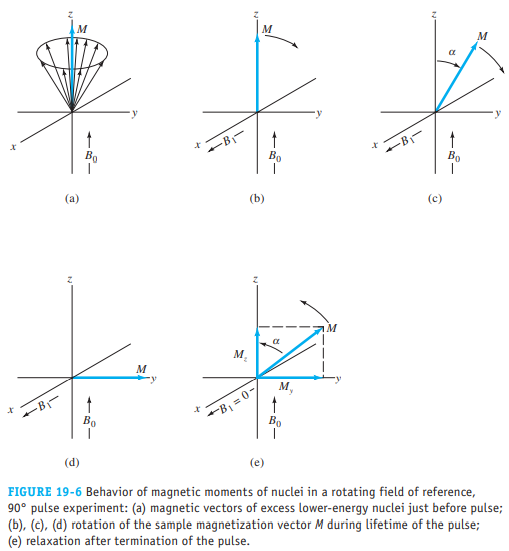
\includegraphics[scale=0.7]{./fig/hc/hc3.png}
\end{center}

\subsection{核磁共振谱的宽度}

依据海森堡测不准原理,我们有以下结论:
\[\Delta E \Delta t \sim h \tag{f}\]

(f)式中,t为横向弛豫用时。
\[\Delta \nu = \frac{\Delta E}{h} \sim \frac{1}{\Delta t} \tag{g}\]

\subsection{脉冲-傅里叶变换核磁共振}

我们知道,有效磁场$\overrightarrow{B_e}$的大小为:
\[|\overrightarrow{B_e}|=\frac{1}{\gamma}\sqrt{(\omega_0-\omega)^2+(\gamma B_{perp})^2}\]

当满足条件$(\gamma B_{perp})^2 \gg (\omega_0-\omega)^2$时,我们可以得到:
\[|\overrightarrow{B_e}| \approx |\overrightarrow{B_{perp}}|\]

这意味着当$\overrightarrow{B_{perp}}$足够大时,一定范围内所有的原子都能发生共振,不需要连续进行扫场或者扫频,打谱时间大大缩短(保证信噪比$\frac{S}{N} \propto \sqrt{n}$足够大),当然这也意味着需要使用短而强的脉冲进行核磁共振。

脉冲-傅里叶变换核磁共振具有以下优点:

\qquad 1、不论同种原子同位素处于分子何处、何种官能团上,都能同时共振;

\qquad 2、用时短,一次测量大概在微秒量级;

\qquad 3、分时装置,接受装置在发射装置后;

\qquad 4、可以使用不同种类的脉冲。

前三点保证了脉冲-傅里叶变换核磁共振用量少、用时短的优点,后两点则使得脉冲-傅里叶变换核磁共振可以完成许多CW(连续波)仪器做不到的事,比如开辟了二维核磁甚至多维核磁的利用。

\section{Nuclear Overhauser effect}

对分子中空间相距比较近(<5 \AA)的两核之一经行辐照,使之达到跃迁的饱和状态,此时记录另一和的核磁共振峰,可发现无此照射时的谱峰强度有所变化,这即使NOE效应,两个核在空间内足够接近是NOE效应的必要条件。

在以谱学方法研究立体化学时核磁共振是最有力的工具,以核磁共振研究立体化学时有以下几种方法:化学位移$\delta$值的变化、耦合常数J(与二面角$\phi$的关系)、NOE等。其中NOE是最有效的方法。

NOE产生的机制是磁性核之间的偶极耦合(dipole coupling),而通过化学键相连的磁性核的自旋-自旋耦合称为标量耦合(scalar coupling),磁性核有磁矩,磁矩与磁矩之间的相互作用正比于$\frac{1}{r^6}$,这也是为什么当两核空间上充分接近时才会有较强的NOE效应的重要原因。

\section{二维核磁}

在一维核磁的部分中,我们知道样品中的磁性核(有磁矩的核)在静电场$B_0$的作用下产生了宏观磁化矢量(宏观磁矩),为使核磁共振发生,需要一个频率恰当的电磁波。射频电磁波是线偏振磁场,可以分解为两个旋转方向相反的圆偏振磁场。其中之一与原子核进动方向相同,该旋转磁场与宏观磁化矢量$M$有相互作用。采用旋转坐标系,旋转坐标系中的旋转磁场$B_{perp}$是相对静止的,沿着x'轴正方向。$M$在$B_{perp}$的作用下,绕着x'轴转动,偏离z轴,产生了横向磁化矢量$M_{perp}$。

当我们使用合适的脉冲,我们可以将宏观磁矩旋转$90^{\circ}$至y'轴上,这样做的好处是宏观磁矩的垂直磁场分量达到最大,在检测信号时更加明显,同时这样也方便检测横向弛豫时间。由于分子内各个方向的磁矩不相同,总有一部分分子运动得快,另一部分分子运动的慢,在绕着磁场进动时,所有分子不都以角速度$2 \pi \nu$转动,但所有宏观磁矩都以$2 \pi \nu$为对称轴在一定角速度内均匀分布,这样的差异将称为我们分析分子中不同精细结构的重要信息。如何利用这些信息,将涉及到\textbf{自旋回波}的内容。

\subsection{自旋回波及其脉冲序列}

首先给出自旋回波的脉冲序列:
\[90^{\circ}_{x'}-DE-180^{\circ}_{x'}-DE, \ AQT\]

接下来我们将分3种情况讨论自旋回波并介绍一些特殊的自旋模式:

\subsubsection{无耦合时的自旋回波}

当施加一个脉冲使得宏观磁矩绕x'轴转$90^{\circ}$到y'轴上后,给其一段时间让其在实验室坐标系下绕z轴旋转,由上部分内容可知,我们设转得最快的宏观磁矩为F、最慢的为S,当施加一个脉冲使得宏观磁矩绕x'轴转$180^{\circ}$到x'Oy'平面y'负半轴区域后,S、F两者位置反转,下一个DE即为第一个DE的逆过程,在DE的最后时刻S、F都重合于y的负半轴。这样对称的过程可以\textbf{消除由于外磁场不均匀带来的误差}。同样的,自旋回波还能使\textbf{化学位移不同的同位素核化学位移重新聚集,这点在后面两种情况依然成立}。

我们可以优化一下这个脉冲序列:
\[90^{\circ}_{x'}-DE-180^{\circ}_{y'}-DE, \ AQT\]

这个优化后的脉冲序列原理于原先的基本一直,但其优势在于经过偶数次DE后宏观磁矩都在y'轴正方向上。我们都知道脉冲让宏观磁矩偏转的角度$\theta$由脉冲作用的宽度(时间)$t_p$调制,但实验中$t_p$不能完全准确,实际的脉冲角度应该为$180 \pm \theta'$,所以,经过偶数次的DE,我们可以消除这一误差来源。

\subsubsection{异核耦合体系的自旋回波} 

异核耦合体系AX的自旋回波基本于无耦合时类似,方便起见,我们只讨论其中的一个原子,对两个不同种的原子核其共振频率相差极大。

假设另外一个核对该原子核的耦合常数为$J$,我们只需将无耦合时的F换成$2 \pi \nu + \frac{J}{2}$,S换成$2\pi \nu - \frac{J}{2}$即可。同样的我们也可以发现自旋回波能将同种原子的不同耦合裂分峰重新聚焦。

\subsubsection{同核耦合体系的自旋回波} 

与异核耦合体系不同,同核体系AA两者的核磁共振频率很相近,这就使得同核耦合体系的自旋回波与异核耦合体系的自旋回波有不同,直接给结论:\textbf{同核耦合体系在经过一个自旋回波过程后,两宏观磁矩的垂直分量关于y'轴负半轴堆成,且均与之成角$2 \pi J \cdot DE$。}因为核磁共振信号强度为$\overrightarrow{B_{perp}}$在y'轴上的投影,所以在此条件下,核磁共振信号强度被$cos(2 \pi J \cdot DE)$调制(modulated),而与化学位移无关,这是后面讨论同核J谱的基础,就这样,我们开始一步步接近核磁共振二维谱了。

\subsubsection{核磁信号的相位被化学位移所调制} 

对异核体系AX,其中A为采集核,X为非采集核,我们讨论以下脉冲序列:
\[90^{\circ}_{x',A}-DE-180^{\circ}_{X}-DE, \ AQT\]

脉冲序列中$180^{\circ}$的脉冲仅作用在非采集核上,绕x'轴和绕y'轴作用类似。

到第一个DE为止都与之前的情况类似,在对非采集核的$180^{\circ}_{X}$后,$2 \pi \nu + \frac{J}{2}$与$2 \pi \nu - \frac{J}{2}$的位置互换,再经过一个DE,两者重新聚合,这时,核磁共振信号强度将被$cos(2 \pi \nu \cdot DE)$调制,即被化学位移调制,而与耦合常数无关。这时讨论异核位移相关谱的基础。

\subsubsection{BIRD脉冲序列} 

BIRD是bilinear rotational decoupling的缩写,译作双线性去耦合。其脉冲序列如下所示:

\[^1H: \qquad 90^{\circ}_{x'}-DE-180^{\circ}_{x'}-DE-90^{\circ}_{x'}, \ AQT\]
\[^{13}C: \qquad \qquad  \qquad \qquad \qquad \qquad \qquad 180^{\circ}_{x'}, \ AQT\]

对$^1H$和对$^{13}C$的$180^{\circ}_{x'}$脉冲是同时加上去的,BIRD脉冲具有以下作用:

\qquad 1、区分$^{13}C-^1H$和$^{12}C-^1H$;

\qquad 2、区分与$^{13}C$直接相连的氢(与$^1J_{CH}$相关)和与$^{13}C$间接接相连的氢(与$^2J_{CH}$、$^3J_{CH}$相关);

\subsubsection{自旋锁定} 

自旋锁定(spin locking)的模型较为简单,大致为对原子核施加一个$90^{\circ}_{x'}$的脉冲使得宏观磁矩转到y'轴正方向,这时,将$\overrightarrow{B_{perp}}$转到y'轴正方向,由于磁矩与磁场重合,他们之间的力矩为0,宏观磁矩不再转动,但弛豫过程还是在发生,所以宏观磁矩的长度会逐渐减小,所以理论上自旋锁定可以用来测定横向弛豫时间。

上面是对孤立磁矩的讨论,下面我们讨论二旋体系的情形:与NOE类似,这两个宏观磁矩都被固定在y'轴上,由于空间上足够接近,两磁矩间存在相互作用,因而构成旋转坐标系下的NOE,称为ROE(rotationg frame Overhauser effect),由ROE产生的二维谱称为ROESY。

\subsubsection{等频混合}

在了解等频混合之前我们首先要了解Hartmann-Hahn匹配(matching)和交叉极化(cross
ing-polarization)

Hartmann-Hahn匹配(matching)的具体内容为:
\[^1H: \qquad 90^{circ}_{x'}-CP-decoupling\]
\[^{13}C: \qquad CP, \ AQT\]

在$^1H$通道首先应用一个$\qquad 90^{circ}_{x'}$将磁矩转到y'轴后,立即加一个磁场将其固定住,同时打开$^{13}C$通道,并调节此通道的射频功率$B_{1C}$满足:
\[\gamma_H B_{1H}=\gamma_C B_{1C} \tag{h}\]

(h)式称为Hartmann-Hahn匹配条件,在此条件下$^{13}C$核与$^1H$核交换能量:由于$^1H$核磁旋比大、丰度高,因此此条件下将检测$^{13}C$核将得到增强性质,检测$^{1}H$核则相反。两核传递能量的过程为交叉极化。

我们知道,不同官能团由于环境的不同,同种同位素的核对应的宏观磁矩旋转频率(即化学位移)$\nu_i$不同,其在旋转坐标系下的旋转频率$\Delta \nu_i:=\nu_0-\nu_i$又称为偏置频率,也不同,这意味着其感受到的相同的射频功率$B_{1_i}$不同,因此将交叉极化推广到同核体系,由于同核体系只有一个射频功率$B_{1}$,不同官能团上的同位素核有不同的偏置频率,Hartmann-Hahn匹配条件难以达到。当然我们知道如果体系越接近Hartmann-Hahn匹配条件的要求,其交叉极化传递越好。

现在考虑两$^1H$核A、X:当满足$\nu_0 \gg \nu_A \ or \ \nu_X$时,$\nu_A$、$\nu_X$可以有以下近似\footnote{Davis D G, Bax A. J Am Chem Soc, 1985,107:2820-2821}:
\[\nu_A= \nu_0 + \frac{{\Delta \nu_A}^2}{2 \nu_0} \qquad \nu_X= \nu_0 + \frac{{\Delta \nu_X}^2}{2 \nu_0}\]

因此我们可以得到:
\[\nu_A-\nu_X=\frac{{\Delta \nu_A}^2-{\Delta \nu_X}^2}{2 \nu_0}\]

当
\[\left | \frac{{\Delta \nu_A}^2-{\Delta \nu_X}^2}{2 \nu_0} \right |<|J_{AX}| \tag{i}\]

满足时:A和X之间能有效传递磁化矢量。其物理意义为:采用强自旋锁定场时,化学位移偏差的影响小于耦合作用的影响,AX体系趋向于AA'体系,即形成一个强耦合体系。对于一个大的耦合体系来说,此耦合体系的各种磁化矢量能通过耦合常数充分相互影响,此时单个自旋模式(single spin mode)已经不复存在,取而代之的是集体自旋模式(collective spin mode)。

由上可知,为实现等频混合,自旋锁定场强度要比ROE强得多。

上述讨论的等频混合是HOHAHA和TOCSY等全相关谱的基础。

\subsection{一些二维核磁谱}

\subsubsection{COSY}

又叫$^1H-^1H \ COSY$,一般反映$^3J_{HH}$耦合关系,少数情况会有长程耦合的相关峰,当$^3J$较小(二面角接近$90^{\circ}$)时可能没有相关峰。

\subsubsection{HETCORE}

又叫$^1H-^{13}C \ COSY$,对$^{13}C$采集信号,一般反映$^1J_{CH}$耦合关系,不能反映季碳,不能反映$^nJ_{CH}$耦合关系。

\subsubsection{HMQC}

又叫HSQC,$^1H-^{13}C \ COSY$,对$^{1}H$采集信号,一般反映$^1J_{CH}$耦合关系,季碳无相关峰,归属完剩下的峰为活泼氢,对于区分非等价亚甲基、解析氢谱重叠有奇效。

\subsubsection{HMBC}

类似$^1H-^{13}C \ COSY$,对$^{1}H$采集信号,一般反映$^nJ_{CH}$耦合关系。

\subsubsection{INADEQUATE}

反映$^1J_{CC}$,准对角线$\omega_1=2\omega_2$,耦合(相邻)的一对碳$\omega_1$(横着的)相同,水平等距得分布在准对角线两侧,其$\omega_2$值对应其$\delta$值。

\subsubsection{TOCSY,HOHAHA}

全相关谱,啥都有($^nJ_{HH}$)。

\subsubsection{NOESY,ROESY}

只要空间相近的两个氢原子就会出峰,与$^1H-^1H \ COSY$有相似性,NOESY主要用于生物大分子,ROESY主要用于小分子。
\chapter{傅里叶变换}
\section{傅里叶变换的部分相关概念及性质}

\subsection{傅里叶级数}

\textit{我们知道,当一个函数$f(x)$满足} \textbf{迪利克雷(Dirichlet)条件} \textit{即在区间${[-\frac{T}{2},\frac{T}{2}]}$上满足} :

\qquad \qquad \text{1、f(x)在区间${[-\frac{T}{2},\frac{T}{2}]}$上连续或者只有有限个第一间断点;}

\qquad \qquad \text{2、f(x)在区间${[-\frac{T}{2},\frac{T}{2}]}$上只有有限个极值点。}

\textit{$f(x)$就可以展开成傅里叶级数} :
\[f(x)=\frac{a_0}{2}+\sum_{n=1}^{+\infty}(a_ncos(n\omega x)+b_nsin(n\omega x)) \tag{a}\]

\textit{其中:}
\[\omega=\frac{2\pi}{T} \qquad a_0=\frac{2}{T}\int_{-\frac{T}{2}}^{\frac{T}{2}}f(x)dx\]
\[a_n=\frac{2}{T}\int_{-\frac{T}{2}}^{\frac{T}{2}}f(x)cos(n\omega x)dx \qquad b_n=\frac{2}{T}\int_{-\frac{T}{2}}^{\frac{T}{2}}f(x)sin(n\omega x)dx\]
\[(n=1,2,3......) \tag{b}\]

\textit{将$cos(n\omega x)$、$sin(n\omega x)$写成复指数形式} :
\[cos(n\omega x)=\frac{e^{in\omega x}+e^{-in\omega x}}{2} \qquad sin(n\omega x)=\frac{e^{in\omega x}-e^{-in\omega x}}{2i} \tag{c}\]

\textit{则} (a) \textit{式可以写成以下形式 }:
\[f(x)=\frac{a_0}{2}+\sum_{n=1}^{+\infty}(\frac{a_n-ib_n}{2}e^{in\omega x}+\frac{a_n+ib_n}{2})e^{-in\omega x} \tag{d}\]

\textit{我们令 }:
\[c_0=\frac{a_0}{2}=\frac{1}{T}\int_{-\frac{T}{2}}^{\frac{T}{2}}f(x)dx\]
\[c_n=\frac{a_n-ib_n}{2}=\frac{1}{T}(\int_{-\frac{T}{2}}^{\frac{T}{2}}f(x)(cos(n\omega x)dx-isin(n\omega x))dx)=\frac{1}{T}\int_{-\frac{T}{2}}^{\frac{T}{2}}f(x)e^{-in\omega x}dx\]
\[c_{-n}=\frac{a_n+ib_n}{2}=\frac{1}{T}(\int_{-\frac{T}{2}}^{\frac{T}{2}}f(x)(cos(n\omega x)dx+isin(n\omega x))dx)=\frac{1}{T}\int_{-\frac{T}{2}}^{\frac{T}{2}}f(x)e^{in\omega x}dx\]
\[(n=1,2,3......)\]

\textit{合并写成 }:
\[c_n=\frac{1}{T}\int_{-\frac{T}{2}}^{\frac{T}{2}}f(x)e^{-in\omega x}dx \qquad (n=\pm 1,\pm 2,\pm 3......) \tag{e}\]

\textit{则}(a)\textit{式可以写成 }:
\[f(x)=c_0+\sum_{n=1}^{+\infty}(c_ne^{i\omega_n x}+c_{-n}e^{-i\omega_n x})=\sum_{n=-\infty}^{+\infty}c_ne^{i\omega_n x} \qquad (\omega_n:=n\omega) \tag{f}\]

\textit{最终,我们得到$f(x)$复指数形式的傅里叶级数 }:
\[f(x)=\sum_{n=-\infty}^{+\infty}(\frac{1}{T}\int_{-\frac{T}{2}}^{\frac{T}{2}}f(y)e^{-i\omega_n y}dy)e^{i\omega_n x} \tag{g}\]

\subsection{傅里叶积分定理}

\textit{在实际的应用中,我们得到的信号曲线不一定是一个周期函数,那么我们有没有办法将一个非周期的函数展开成傅里叶级数呢} ?

\textit{对于一个定义在实数轴上的非周期的函数,我们可以认为它的周期是无穷大,对此我们将把能展开成傅里叶级数的周期函数延拓到整个实数轴上,再将其周期取为无穷大。}

\textit{将$f(x)$按周期$T$在实数域上做延拓的到函数$f_T(x)$ }:
\[ f_T(x) := \left\{
\begin{array}{rl}
f(x) & \text{if } x \in [-\frac{T}{2},\frac{T}{2}]\\
f_T(x \pm T) & \text{if } x \notin [-\frac{T}{2},\frac{T}{2}] 
\end{array} \right. \]

\textit{当$T \rightarrow \infty$时,我们可以得到 }:
\[\lim_{T \rightarrow \infty}{f_T(x)=f(x)}\]

\textit{则,由$(g)$式可知,对于一个可以展开成傅里叶级数且其周期$T$无穷大的函数,其傅里叶级数可以写成 }:
\[f(x)=\lim_{T \rightarrow \infty}\frac{1}{T}\sum_{n=-\infty}^{+\infty}(\int_{-\frac{T}{2}}^{\frac{T}{2}}f(y)e^{-i\omega_n y}dy)e^{i\omega_n x} \tag{h}\]

\textit{这里,我们定义一个新的量$\Delta{\omega}$ }:
\[\Delta{\omega}:=\omega_n-\omega_{n-1}=\omega=\frac{2\pi}{T}\]

\textit{则$(h)$式可以写成 }:
\[f(x)=\lim_{\Delta{\omega} \rightarrow 0}\frac{1}{2\pi}\sum_{n=-\infty}^{+\infty}(\int_{-\frac{T}{2}}^{\frac{T}{2}}f(y)e^{-i\omega_n y}dy)e^{i\omega_n x}\Delta{\omega} \tag{i}\]

\textit{由积分的定义式我们可以知道$(i)$式最终可以写成 }:
\[f(x)=\frac{1}{2\pi}\int_{-\infty}^{+\infty}(\int_{-\infty}^{+\infty}f(y)e^{-i\omega y}dy)e^{i\omega x}d\omega \tag{j}\]

\textit{上面我们不严格地推导处理傅里叶积分公式,下面我们给出傅里叶积分公式的严格定义 }:

\textbf{傅里叶积分定理}

\text{若$f(x)$在${(-\infty,+\infty)}$满足:}

\qquad \qquad \text{在任一有限区间上满足迪利克雷条件;}

\qquad \qquad \text{在${(-\infty,+\infty)}$上绝对可积(即$\int_{-\infty}^{+\infty}|f(x)|dx$收敛);}

\text{当$f(x)$在点$x=x_0$处连续时,则有:}
\[\frac{1}{2\pi}\int_{-\infty}^{+\infty}(\int_{-\infty}^{+\infty}f(y)e^{-i\omega y}dy)e^{i\omega x_0}d\omega=f(x_0)\]

\text{当$f(x)$在点$x=x_0$处不连续时,则有:}
\[\frac{1}{2\pi}\int_{-\infty}^{+\infty}(\int_{-\infty}^{+\infty}f(y)e^{-i\omega y}dy)e^{i\omega x_0}d\omega=\frac{1}{2}\left ( \lim_{x \rightarrow x_0^-}{f(x)}+\lim_{x \rightarrow x_0^+}{f(x)} \right )\]

\subsection{傅里叶变换的概念}

\textbf{定义} \text{如果$f(t)$满足傅里叶积分定理,设} :
\[F(\omega)=\int_{-\infty}^{+\infty}f(t)e^{-i\omega t}dt \tag{1}\] 
\[f(t)=\frac{1}{2\pi}\int_{-\infty}^{+\infty}F(\omega)e^{i\omega t}d\omega \tag{2}\]

\text{则称$F(\omega)$为$f(t)$的象函数,称(1)式为$f(t)$的傅里叶变换式,记为:}
\[F(\omega)=\mathcal{F}[f(t)]\]

\text{则称$f(t)$为$F(\omega)$的象原函数,称(2)式为$F(\omega)$的傅里叶逆变换式,记为:}
\[f(t)=\mathcal{F}^{-1}[F(\omega)]\]

\subsection{δ函数及其傅里叶变换}

\textit{单位脉冲函数是英国物理学家狄拉克(Dirac)在20世纪20年代引人的,用于描述瞬间或空间几何点上的物理量。例如,瞬时的冲击力、脉冲电流或电压等急速变化的物理量,以及质点的质量分布、点电荷的电量分布等在空间或时间上高度集中的物理量。脉冲函数也称$\delta$函数。}

\textbf{定义} \qquad \text{若在一维空间中,自变量为时间t的函数$\delta(t)$,满足下述两个条件:}
\[\delta(t)=\left\{
\begin{array}{rl}
0 & \text{if } x \neq 0\\
1 & \text{if } x=0
\end{array} \right. \tag{1}\]
\[\int_{-\infty}^{+\infty}\delta(t)dt=1 \tag{2}\]

\textit{不论是$\delta$函数还是有延时的$\delta$函数$(\delta(t-t_0))$,都有如下重要的性质} (\textbf{筛选性质}) :

\[\int_{-\infty}^{+\infty}\delta(t-t_0)f(t)dt=f(t_0) \tag{k}\]

\textit{利用这个性质,我们可以对单位脉冲函数求其傅里叶变换及傅里叶逆变换} :

\[F(\omega)=\mathcal{F}[\delta(t-t_0)]=\int_{-\infty}^{+\infty}\delta(t-t_0)e^{-i\omega t}dt=e^{-i\omega t_0}\]

\textit{令$F(\omega)=2\pi \delta(\omega-\omega_0)$则有} : 
\[f(t)=\mathcal{F}^{-1}[2\pi \delta(\omega-\omega_0)]=\frac{1}{2\pi}\int_{-\infty}^{+\infty}2\pi \delta(\omega-\omega_0)e^{i\omega t}d\omega=e^{i\omega_0 t}\]

\textit{这是我们得到两对傅里叶变换对} :

\[\delta(t-t_0) \ and \ e^{-i\omega t_0} \quad,\quad e^{i\omega_0 t} \ and \ 2\pi \delta(\omega-\omega_0) \tag{l}\]

\textit{特别的,我们令$t_0=0,\omega_0=0$,则有以下两个重要的傅里叶变换对} :

\[\delta(t) \ and \ 1 \quad,\quad 1 \ and \ 2\pi \delta(\omega) \tag{m}\]

\textit{此外$\delta$函数还有另一个性质} :

\textbf{定义} \qquad \textit{设函数$u(t)$为单位阶跃函数,即} :

\[u(t)=\left\{ \begin{array}{rl}
1 & \text{if } x>0 \\
0 & \text{if } x<0 
\end{array} \right. \]

\textit{则我们可以获得以下关系式 }:

\[\frac{\mathrm{d}}{\mathrm{d} t}u(t)=\delta(t)\]

\[F(\omega)=\mathcal{F}[u(t)]=\int_{-\infty}^{+\infty}\frac{1+sgn(t)}{2}e^{-i\omega t}dt=\frac{1}{i\omega}+\pi\delta(\omega)\]

\[u(t)=\mathcal{F}^{-1}[F(\omega)]=\frac{1}{2\pi}\int_{-\infty}^{+\infty}\Bigl(\frac{1}{i\omega}+\pi\delta(\omega) \Bigl)e^{i\omega t}dt=\frac{1}{2}+\frac{1}{2\pi}\int_{-\infty}^{+\infty}\frac{sin\omega}{\omega}d\omega \tag{n}\]

\textit{$\delta$函数并不是严格意义上数域到数域的函数,而是个定义在函数空间上的泛函,它的引入扩充了傅里叶变换的适用范围,使得一些不满足条件$\int_{-\infty}^{+\infty}|f(x)|dx<+\infty$的函数,如常值函数、符号函数、单位阶跃函数、正弦函数、余弦函数都能进行广义傅里叶变换.}

\textit{例如下面两个例子以及上面的常值函数以及单位阶跃函数 }:

\[\mathcal{F}[cos(\omega_0t)]=\pi[\delta(\omega+\omega_0)+\delta(\omega-\omega_0)] \tag{o1}\]

\[\mathcal{F}[sin(\omega_0t)]=i\pi[\delta(\omega+\omega_0)-\delta(\omega-\omega_0)] \tag{o2}\]

\subsection{傅里叶变换的性质}

\textit{这一小节我们介绍傅里叶变换的几个性质,为方便起见,我们规定在该小节中处理的函数均满足傅里叶积分定理的条件。}

\text{1.线性性质}

\[\mathcal{F}[af_1(t)+bf_2(t)]=a\mathcal{F}[f_1(t)]+b\mathcal{F}[f_2(t)]\]
\[\mathcal{F}^{-1}[af_1(t)+bf_2(t)]=a\mathcal{F}^{-1}[f_1(t)]+b\mathcal{F}^{-1}[f_2(t)]\]
\[(a,b \in \mathcal{R})\]

\text{2.位移性质}
\[\mathcal{F}[f(t \pm t_0)]=e^{\pm i\omega t_0}\mathcal{F}[f(t)]\]
\[\mathcal{F}^{-1}[f(t \pm t_0)]=e^{\mp i\omega t_0}\mathcal{F}^{-1}[f(t)]\]

\text{3.微分性质}

\textit{若$f^{(k)}(x)$在$(-\infty,+\infty)$$(k=0,1,2,...,n-1)$连续或者只有有限个间断点,且满足 }
\[\lim_{|t|\rightarrow +\infty}f^{(k)}(t)=0\]

\textit{则有 }:
\[\mathcal{F}[f^{(n)}(t)]=(i\omega)^n \mathcal{F}[f(t)]\]
\[\frac{\mathrm {d}^n}{\mathrm {d} \omega^n} \mathcal{F}[f(t)]=(-i)^n \mathcal{F}[t^nf(t)]\]

\text{4.积分性质}

\textit{当$t \rightarrow +\infty$时,$\int_{-\infty}^{t}f(t)dt \rightarrow 0$,则 }:
\[ \mathcal{F}[\int_{-\infty}^{t}f(t)dt]=\frac{1}{i\omega}\mathcal{F}[f(t)]\]

\text{5.乘积定理}

\textit{若$F_1(\omega)=\mathcal{F}[f_1(t)]$,$F_2(\omega)=\mathcal{F}[f_2(t)]$,则 }:

\[\int_{-\infty}^{+\infty}\overline{f_1(t)}f_2(t)dt=\frac{1}{2\pi}\int_{-\infty}^{+\infty}\overline{F_1(\omega)}F_2(\omega)d\omega\]
\[\int_{-\infty}^{+\infty}f_1(t)\overline{f_2(t)}dt=\frac{1}{2\pi}\int_{-\infty}^{+\infty}F_1(\omega)\overline{F_2(\omega)}d\omega\]

\text{6.能量积分}

\textbf{Parseval等式} \qquad \textit{若$F(\omega)=\mathcal{F}[f(t)]$,则 }:

\[\int_{-\infty}^{+\infty}[f(t)]^2dt=\frac{1}{2\pi}\int_{-\infty}^{+\infty}[F(\omega)]^2d\omega:=\frac{1}{2\pi}\int_{-\infty}^{+\infty}S(\omega)d\omega\]

\subsection{卷积与卷积定理}

\textit{若已知函数$f_1(t)$、$f_2(t)$,则我们定义卷积为 }:

\[f_1(t)\ast f_2(t):=\int_{-\infty}^{+\infty}f_1(\tau)f_2(t-\tau)d\tau \tag{p}\] 

\textit{容易验证卷积运算满足 }:

\textit{1.交换律:$f_1(t)\ast f_2(t)=f_2(t)\ast f_1(t)$}

\textit{2.结合律:$(f_1(t) \ast f_2(t)) \ast f_3(t)=f_1(t) \ast (f_2(t) \ast f_3(t))$}

\textit{3.对加法的分配律:$f_1(t) \ast (f_2(t)+f_3(t))=f_1(t) \ast f_2(t)+f_1(t) \ast f_3(t)$}

\textit{此外,卷积运算还满足以下性质 } :

\textit{卷积的数乘 }:

\[a[f_1(t)\ast f_2(t)]=[af_1(t)]\ast f_2(t)=f_1(t)\ast [af_2(t)] \qquad (a \in \mathcal{R})\]

\textit{卷积的微分 }:

\[\frac{\mathrm {d}}{\mathrm {d}x}[f_1(t)\ast f_2(t)]=[\frac{\mathrm {d}}{\mathrm {d}x}f_1(t)]\ast f_2(t)=f_1(t)\ast\frac{\mathrm {d}}{\mathrm {d}x}[ f_2(t)]\]

\textit{卷积的积分 }:

\[\int_{-\infty}^{t}[f_1(\phi)\ast f_2(\phi)]=[\int_{-\infty}^{t}f_1(\phi)]\ast f_2(\phi)=f_1(\phi)\ast [\int_{-\infty}^{t}f_2(\phi)]\]

\textit{卷积不等式 }:

\[|f_1(t)\ast f_2(t)| \leqslant |f_1(t)|\ast |f_2(t)|\]

\textit{与$\delta$函数相关的性质 }:

\[f(t) \ast \delta(t)=f(t)\]

\textbf{卷积定理} \qquad \textit{若$f_1(t)$和$f_2(t)$满足傅里叶积分定理的条件,则有 }:

\[\mathcal{F}[f_1(t) \ast f_2(t)]=\mathcal{F}[f_1(t)] \cdot \mathcal{F}[f_2(t)]\]

\subsection{相关函数}

\textit{给定两函数$f_1(t)$、$f_2(t)$,则定义互相关函数 }:

\[R_{12}(\tau):=\int_{-\infty}^{+\infty}f_1(t)f_2(t+\tau)dt \qquad R_{21}(\tau):=\int_{-\infty}^{+\infty}f_1(t+\tau)f_2(t)dt\]

\textit{当$f_1(t)=f_2(t)$时,则定义自相关函数 }:

\[R(\tau):=\int_{-\infty}^{+\infty}f(t)f(t+\tau)dt\]

\textit{关于互相关函数有如下性质 }:

\[R_{21}(\tau)=R_{12}(-\tau)\]

\textit{若令乘积定理中实函数$f_1(t)=f_1(t)$,$f_2(t)=f_2(t+\tau)$,则有 }:

\[\int_{-\infty}^{+\infty}f_1(t)f_2(t+\tau)dt=\frac{1}{2\pi}\int_{-\infty}^{+\infty}\overline{F_1(\omega)}F_2(\omega)e^{i\tau \omega}d\omega :=\frac{1}{2\pi}\int_{-\infty}^{+\infty}S_{12}(\omega)e^{i\tau \omega}d\omega\]

\[R_{12}(\tau)=\frac{1}{2\pi}\int_{-\infty}^{+\infty}S_{12}(\omega)e^{i\tau \omega}d\omega \qquad S_{12}(\omega)=\overline{S_{21}(\omega)} \tag{q}\]

\textit{当$f_1(t)=f_2(t)$时} (q) \textit{式可做出相应的简化。}

\section{傅里叶变换的应用}

\subsection{周期函数与离散频谱}

\textit{对一个周期为$T$的函数$f(t)$其傅里叶级数为 }:

\[f(t)=\sum_{n=-\infty}^{+\infty}g(n)e^{in\omega_0 t} \]

\textit{对上式两边同时取傅里叶变换,并认为系数项不为时间$t$的函数,由此可得 }:

\[F(\omega)=\mathcal{F}[f(t)]=\int_{-\infty}^{+\infty}[\sum_{n=-\infty}^{+\infty}g(n)e^{in\omega_0 t}]e^{-i\omega t}dt=2\pi\sum_{n=-\infty}^{+\infty}g(n)\delta(\omega-n\omega_0) \tag{r}\]

\subsection{非周期函数与连续频谱}

\textit{对非周期函数$f(t)$,若其满足傅里叶积分定理条件,则在$f(t)$的连续点处,有 }:

\[f(t)=\frac{1}{2\pi}\int_{-\infty}^{+\infty}F(\omega)e^{i\omega t}d\omega\]

\textit{其傅里叶变换式为} :

\[F(\omega)=\int_{-\infty}^{+\infty}f(t)e^{-i\omega t}dt\] 

\textit{在频谱分析中,傅里叶变换式$F(\omega)$又称为$f(t)$的频谱函数,频谱函数的模$|F(\omega)|$称为$f(t)$的振幅频谱(亦可简称为频谱)。在傅里叶积分中当$n\rightarrow +\infty$时,频率间隔$\Delta \omega $成为$d\omega$,$\omega$为连续变量,故称$|F(\omega)|$为连续频谱。对一个时间函数$f(t)$做傅里叶变换,就是求$f(t)$的频谱。}
\chapter{杂碎}
\section{二阶线性常微分方程找特解}
\textit{Now, we want to find a special solution for following ordinary differential equation} :

\[\frac{\mathrm{d}^2 y}{\mathrm{d} x^2} + p(x) \frac{\mathrm{d} y}{\mathrm{d} x}+q(x)y=f(x) \tag{a} \]

\textit{Assume the general solution of this ordinary differential equation is} y(x)= $c_1$ $y_1$(x)+$c_2$ $y_2$(x).

\textit{Then we assume the special solution of this ordinary differential equation is} $y^*$(x)= $c_1$(x) $y_1$(x)+$c_2$(x) $y_2$(x).

\textit{Bringing this special solution} $y^*$(x) \textit{into the equation} (a) \textit{, we can get} :

\[\sum_{1}^{2} \left (\frac{\mathrm{d}^2 c_i}{\mathrm{d} x^2} y_i +2\frac{\mathrm{d} c_i}{\mathrm{d} x} \frac{\mathrm{d} y_i}{\mathrm{d} x}+ c_i \frac{\mathrm{d}^2 y_i}{\mathrm{d} x^2} + p( \frac{\mathrm{d} c_i}{\mathrm{d} x} y_i + c_i \frac{\mathrm{d} y_i}{\mathrm{d} x})+qc_iy_i \right)=f(x)\]

\[\sum_{1}^{2} \left ( (\frac{\mathrm{d}^2 c_i}{\mathrm{d} x^2} y_i +2\frac{\mathrm{d} c_i}{\mathrm{d} x} \frac{\mathrm{d} y_i}{\mathrm{d} x}+p \frac{\mathrm{d} c_i}{\mathrm{d} x} y_i + (c_i \frac{\mathrm{d}^2 y_i}{\mathrm{d} x^2}+pc_i \frac{\mathrm{d} y_i}{\mathrm{d} x}+qc_iy_i) \right)=f(x) \quad (b) \]

\textit{Since the solutions of this ordinary differential equation satisfy following equation} :

\[\sum_{1}^{2} \left ( \frac{\mathrm{d}^2 y_i}{\mathrm{d} x^2} + p(x) \frac{\mathrm{d} y_i}{\mathrm{d} x}+q(x)y_i \right ) =f(x) \tag{c}\]

\textit{We can simplify the equation} (b) :

\[\sum_{1}^{2} \left(\frac{\mathrm{d}^2 c_i}{\mathrm{d} x^2} y_i +2\frac{\mathrm{d} c_i}{\mathrm{d} x} \frac{\mathrm{d} y_i}{\mathrm{d} x}+p(x) \frac{\mathrm{d} c_i}{\mathrm{d} x} y_i) \right)=f(x) \tag{d} \]

\textit{It doesn't matter that we can assume} :

\[\sum_{1}^{2} \frac{\mathrm{d} c_i}{\mathrm{d} x} y_i =0 \tag{e} \]

\textit{We can also get following equation from equation} (e) :

\[\sum_{1}^{2} \left( \frac{\mathrm{d}^2 c_i}{\mathrm{d} x^2} y_i +\frac{\mathrm{d} c_i}{\mathrm{d} x} \frac{\mathrm{d} y_i}{\mathrm{d} x} \right)=0 \tag{f}\]

\textit{Bring equation} (e) \textit{and} (f) \textit{into equation} (d) \textit{,we can get} :

\[\sum_{1}^{2} \frac{\mathrm{d} c_i}{\mathrm{d} x} \frac{\mathrm{d} y_i}{\mathrm{d} x}=f(x) \tag{g}\]

\textit{Combine equation} (e) and \textit{equation} (g) \textit{,we can get} :

\[\begin{pmatrix} y_1 & y_2 \\ {y_1}' & {y_2}' \end{pmatrix} \begin{pmatrix} {c_1}' \\ {c_2}' \end{pmatrix} = \begin{pmatrix} 0 \\ f(x) \end{pmatrix} \tag{h} \]

\textit{Solve this system of equations, we can work out following two equations}:

\[ {c_1}'=\frac {\begin{pmatrix} 0 & y_2 \\ f(x) & {y_2}' \end{pmatrix}} {\begin{pmatrix} y_1 & y_2 \\ {y_1}' & {y_2}' \end{pmatrix}} =\frac {-y_2 f(x)}{y_1 {y_2}' - y_2 {y_1}'} \tag{i1} \]

\[ {c_2}'=\frac {\begin{pmatrix} y_1 & 0 \\ {y_1}' & f(x) \end{pmatrix}} {\begin{pmatrix} y_1 & y_2 \\ {y_1}' & {y_2}' \end{pmatrix}} =\frac {y_1 f(x)}{y_1 {y_2}' - y_2 {y_1}'} \tag{i2} \]

\textit{Finally,we can get the special solution of equation} (a) :

\[y^*=\int{\frac {-y_2 f(x)}{y_1 {y_2}' - y_2 {y_1}'}} y_1 + \int{\frac {y_1 f(x)}{y_1 {y_2}' - y_2 {y_1}'}} y_2 \tag{j} \]


\section{Wronskian行列式找特解}
找特解的时候我们一般采用常数变易法,我们假设我们要处理的线性非齐次常系数微分方程为
\[\sum_{i=0}^na_iy^{(i)}=f \qquad (\text{记} \ y^{(0)}=y) \tag{*}\]
我们记对应齐次方程(无简并特征根)的通解的常数易变为,其中$y_i(t)$满足齐次方程。
\[y(t)=\sum_{j=1}^nv_j(t)y_j(t) \tag{1}\]
将(1)将代入(*)式,得到
\[\sum_{i=0}^na_i\sum_{j=1}^n\left(\sum_{k=0}^iC_i^kv_j^{(k)}y_j^{(i-k)}\right)=f\]
按照$v_j^{(i)}$做整理得到
\[\sum_{j=1}^n\sum_{i=0}^nv_j^{(i)}\left(\sum_{k=i}^{n}a_{k}C_{k}^iy_j^{(k-i)}\right)=f\]
我们会发现,所以含$v_i^{(0)}$的项抵消了,因为$v_i^{(0)}$项的系数是下式
\[\sum_{j=1}^nv_j^{(0)}\left(\sum_{k=0}^{n}a_{k}y_j^{(k-i)}\right)=0\]
所以有
\[\sum_{j=1}^n\sum_{i=1}^nv_j^{(i)}\left(\sum_{k=i}^{n}a_{k}C_{k}^iy_j^{(k-i)}\right)=f\]
我们取含$v_j'$的项为$f$,其余的项为0。
\[\sum_{j=1}^nv_j'\left(\sum_{k=1}^{n}a_{k}C_{k}^1y_j^{(k-1)}\right)=f \qquad \sum_{j=1}^nv_j^{(i)}\left(\sum_{k=i}^{n}a_{k}C_{k}^iy_j^{(k-i)}\right)=0 \quad (i=2,3,\cdots,n)\]
改写方程
\[\sum_{k=1}^{n}\sum_{j=1}^nv_j'\left(a_{k}C_{k}^1y_j^{(k-1)}\right)=f\]
容易看出,上式可以进一步改写成
\[
\begin{pmatrix}
    a_{1}C_{1}^1y_1 & a_{1}C_{1}^1y_2 & \cdots & a_{1}C_{1}^1y_n \\
    a_{2}C_{2}^1y'_1 & a_{2}C_{2}^1y'_2 & \cdots & a_{2}C_{2}^1y'_n \\
    \vdots & \vdots & \ddots & \vdots \\
    a_{n}C_{n}^1y^{(n-1)}_1 & a_{n}C_{n}^1y^{(n-1)}_2 & \cdots & a_{n}C_{n}^1y^{(n-1)}_n
\end{pmatrix}    
\begin{pmatrix}
    v'_1 \\ v'_2 \\ \vdots \\ v'_n \\
\end{pmatrix}   
=
\begin{pmatrix}
    0 \\ 0 \\ \vdots \\ f \\
\end{pmatrix}     
\]
根据线性方程组的性质,我们知道,上式和下式的解相同:
\[
\begin{pmatrix}
    y_1 & y_2 & \cdots & y_n \\
    y'_1 & y'_2 & \cdots & y'_n \\
    \vdots & \vdots & \ddots & \vdots \\
    y^{(n-1)}_1 & y^{(n-1)}_2 & \cdots & y^{(n-1)}_n
\end{pmatrix}    
\begin{pmatrix}
    v'_1 \\ v'_2 \\ \vdots \\ v'_n \\
\end{pmatrix}   
=
\begin{pmatrix}
    0 \\ 0 \\ \vdots \\ f' \\
\end{pmatrix}     
\qquad \text{where} \ f'=\frac{f}{a_{n}C_{n}^1}=\frac{f}{na_{n}}
\]
为了保有方程的形式,我们可以重新将系数$na_n$并入一开始求算的通解中,即
\[y_j:=na_ny_j \qquad (j=1,2,\cdots,n)\]
则方程组可以写成
\[
\begin{pmatrix}
    y_1 & y_2 & \cdots & y_n \\
    y'_1 & y'_2 & \cdots & y'_n \\
    \vdots & \vdots & \ddots & \vdots \\
    y^{(n-1)}_1 & y^{(n-1)}_2 & \cdots & y^{(n-1)}_n
\end{pmatrix}    
\begin{pmatrix}
    v'_1 \\ v'_2 \\ \vdots \\ v'_n \\
\end{pmatrix}   
=
\begin{pmatrix}
    0 \\ 0 \\ \vdots \\ f \\
\end{pmatrix}     
\]
如果我们记
\[
\mathcal{W}(s)=
\begin{vmatrix}
    y_1(s) & y_2(s) & \cdots & y_n(s) \\
    y'_1(s) & y'_2(s) & \cdots & y'_n(s) \\
    \vdots & \vdots & \ddots & \vdots \\
    y^{(n-1)}_1(s) & y^{(n-1)}_2(s) & \cdots & y^{(n-1)}_n(s)
\end{vmatrix}  
\]
\[
\mathcal{W}_i(s)=
\begin{vmatrix}
    y_1(s) & y_2(s) & \cdots & y_{i-1}(s) & 0 & y_{i+1}(s) & \cdots & y_n(s) \\
    y'_1(s) & y'_2(s) & \cdots & y'_{i-1}(s) & 0 & y'_{i+1}(s) & \cdots & y'_n(s) \\
    \vdots & \vdots & \cdots & \vdots & \vdots & \vdots & \cdots & \vdots \\
    y^{(n-1)}_1(s) & y^{(n-1)}_2(s) & \cdots & y^{(n-1)}_{i-1}(s) & f(s) & y^{(n-1)}_{i+1}(s) & \cdots & y^{(n-1)}_n(s)
\end{vmatrix} 
\]
由$Cramer$法则可以知道
\[v_i'(s)=\frac{\mathcal{W}_i(s)}{\mathcal{W}(s)} \qquad (i=1,2,\cdots,n)\]
故
\[v_i(t)=\int v_i'(s)ds=\int \frac{\mathcal{W}_i(s)}{\mathcal{W}(s)}ds\]
我们也可以将$f(s)$提出,记
\[
\mathcal{W}_{0,i}(s):=f(s)
\begin{vmatrix}
    y_1(s) & y_2(s) & \cdots & y_{i-1}(s) & 0 & y_{i+1}(s) & \cdots & y_n(s) \\
    y'_1(s) & y'_2(s) & \cdots & y'_{i-1}(s) & 0 & y'_{i+1}(s) & \cdots & y'_n(s) \\
    \vdots & \vdots & \cdots & \vdots & \vdots & \vdots & \cdots & \vdots \\
    y^{(n-1)}_1(s) & y^{(n-1)}_2(s) & \cdots & y^{(n-1)}_{i-1}(s) & 1 & y^{(n-1)}_{i+1}(s) & \cdots & y^{(n-1)}_n(s)
\end{vmatrix} 
\]
则有
\[v_i(t)=\int v_i'(s)ds=\int \frac{f(s)\mathcal{W}_{0,i}(s)}{\mathcal{W}(s)}ds\]

\section{TST推导}\textit{Basic hypothesis:}

A. Before dividing surface, transition-state and reactant obey Maxwell Boltzmann distribution;

B. After dividing surface, the reaction between transition-state and product is irreversible reaction, and once molecules go through dividing surface we consider they must become product.

We call reactant as R and transition-state as TS.
\[-\frac{\mathrm{d} {[R]}}{\mathrm{d} t} = k_f[R]-k_b[TS] \tag{a}\]
\[-\frac{\mathrm{d} {[TS]}}{\mathrm{d} t} = k_2[TS]-k_f[R]+k_b[TS] \tag{b}\]

Because of hypothesis 1, we can get following equation:
\[k_f[R]-k_b[TS]=0 \qquad \Rightarrow \qquad [TS]=\frac{k_f}{k_b}[R]\]

And we consider probability flow as a constant, also the change on R and TS is relative tiny:
\[\frac{\mathrm{d} {[R]}}{\mathrm{d} t} = \frac{\mathrm{d} {[TS]}}{\mathrm{d} t}\]
then:
\[-\frac{\mathrm{d} {[TS]}}{\mathrm{d} t} = k_2[TS]+k_b[TS]-k_f[R]=k_2[TS]=\frac{k_fk_2}{k_b}[R]\]

\[-\frac{\mathrm{d} {[R]}}{\mathrm{d} t} = \frac{k_fk_2}{k_b}[R] :=k[R]\]

Since concentration is proportional to partition function, and adjust transition-state and reactant to the same energy zero point, we can write equation (b) as follows:
\[\frac{k_f}{k_b}= \frac{Q_{TS}}{Q_R} e^{\frac{E}{kT}} \tag{c} \]

Consider the neighbourhood of transition-state along reaction pathway, take a tiny length dl out, on \textit{dl} we think reaction rate is a constant approximatively. Then we can get:

\[\frac{1}{k_2}= \tau = \frac{dl}{v} = \frac{dl}{<v>} \tag {d} \]

Put equation (c) and equation (d) together, we get:

\[k= \frac{Q_{TS}}{Q_R} e^{\frac{E}{kT}} \frac{<v>}{dl} \tag{e} \]

Sinse we consider the neighbourhood of transition-state, we can consider the molecules are free particles, let's consider the one-dimension Maxwell Distribution of Speed:

\[<v> = \int_{0}^{\infty}\sqrt{\frac{\mu}{2 \pi kT}}ve^{ - \frac{\mu v^2}{2kT}}dv \tag{f} \]

Easily, we can finally get the expression of <v>:

\[<v>=\sqrt{\frac{2kT}{\pi \mu}} \tag{g}\]

Also, we can get the expression of $k$:

\[k= \frac{Q_{TS}}{Q_R} e^{\frac{E}{kT}} \sqrt{\frac{2kT}{\pi \mu}} \frac{1}{dl} \tag{h} \]

As we all know, partition function can be calculated by Hamiltonian:

\[Q_i = \sum_j<\psi_j|e^{\beta \hat{H_i}}|\psi_j>=Tr{(e^{\beta \hat{H_i}})} \quad (i=TS,R) \qquad \text{where} \quad \bra{\phi_i}\ket{\phi_j}=\delta_{ij} \tag{i}\]

We can separate transition-state's Hamiltonian as one along dividing surface and the other along reaction pathway, here we assume these two dimensions are independent:

\[Q_{TS} =Tr{(e^{\beta (\hat{H_{DS}}+\hat{H_{RP}})})}=Tr{(e^{\beta \hat{H_{DS}}})}Tr{(e^{\beta \hat{H_{RP}}})}=Q_{DS}Q_{RP} \tag{j}\]

Also, consider the molecules are free particle, and the reaction is irreverible, we get following in phase space:

\[Q_{RP}=\frac{1}{2}Q_{FP}=\frac{1}{h}\int_{-dl}^{0}\int_{-\infty}^{\infty}e^{\frac{p^2}{2 \mu kT}}dxdp \tag{k}\]

Then ,we get:

\[Q_{RP}=\frac{dl}{2h}\sqrt{2 \pi \mu kT} \tag{l} \]

Finally, we get the expression of $k$ as follows:

\[k=\frac{kT}{h} \frac{Q_{DS}}{Q_R} e^{\frac{E}{kT}} \tag{*} \]

By the way, the energy E here refers to the differential value between transition-state's vibrational level zero energy point and reaction's.

\section{随机游走均方末端距}
对于流体中某面元上的扩散速率,我们知道其正比于该流体的数量密度对运动位移矢量的偏导:
\[J=-D\nabla\rho \tag{a}\]

我们采用拉格朗日法研究扩散时,溶质密度随时间的变化,这里我们给出密度在拉格朗日法下的函数表示:
\[\rho=\rho(\vec{x},t)\]

在$\vec{x}$方向上我们考虑体积元$Ad\vec{x}$内的密度变化,在体积元中,我们可以得知,扩散速率场与面元的乘积未体积元中粒子数的变化量,与密度随时间的变化成正比,系数为-1:
\[\frac{\partial \rho}{\partial t}=-\lim_{\partial \vec{x} \rightarrow 0} \frac{[J(\vec{x}+\partial \vec{x})-J(\vec{x})] \cdot A}{\partial \vec{x} \cdot A} =-\nabla \cdot J \tag{b}\]

结合(a)、(b)两式,我们可以得到含时的扩散方程(time-dependent diffusion equation):
\[\frac{\partial \rho}{\partial t}=D\nabla^2\rho \tag{c}\]

这里我们认为扩散的体系是各向同性的,则扩散系数为一常数,反之则为$\vec{x}$的函数。

函数$\rho(\vec{x},t)$处理起来不便,我们可以考虑对其分量进行处理并使用傅里叶变换在其动量空间上进行处理,下列$x$与$k$表示沿着同一分量的位移与动量:

\[\rho(x,t)=\int_{-\infty}^{+\infty}\rho_k(t)e^{-ikx}dk\]

\[\frac{\partial \rho}{\partial t}=\int_{-\infty}^{+\infty}\frac{\mathrm{d} \rho_k(t)}{\mathrm dt}e^{-ikx}dk\]

\[\nabla^2\rho=\int_{-\infty}^{+\infty}\rho_k(t)\nabla^2 e^{-ikx}dk=\int_{-\infty}^{+\infty}-k^2\rho_k(t)e^{-ikx}dk\]

易得:
\[\int_{-\infty}^{+\infty}(\frac{\mathrm{d} \rho_k(t)}{\mathrm dt}+Dk^2\rho_k(t))e^{-ikx}dk=0\]

由$t$的任意性,我们可以得到:
\[\frac{\mathrm{d} \rho_k(t)}{\mathrm dt}+Dk^2\rho_k(t)=0 \tag{d}\]

解该微分方程我们得到以下结果:
\[\rho_k(t)=\rho_k(0)e^{-Dk^2t}\]

其中$\rho_k(0)$可以通过边界条件$\rho(\vec{0},0)=\delta(0)$确定:

\[\rho_k(t)=\frac{1}{2\pi}\int_{-\infty}^{+\infty}\rho(x,t)e^{ikx}dk\]

\[\rho_k(0)=\lim_{t \rightarrow 0}\rho_k(t)=\lim_{t \rightarrow 0}\frac{1}{2\pi}\int_{-\infty}^{+\infty}\rho(x,t)e^{ikx}dk\]

\[\lim_{t \rightarrow 0}\frac{1}{2\pi}\int_{-\infty}^{+\infty}\rho(x,t)e^{ikx}dk=\frac{1}{2\pi}\int_{-\infty}^{+\infty}\lim_{t \rightarrow 0}\rho(x,t)e^{ikx}dk\]

\[\frac{1}{2\pi}\int_{-\infty}^{+\infty}\lim_{t \rightarrow 0}\rho(x,t)e^{ikx}dk=\frac{1}{2\pi}\int_{-\infty}^{+\infty}\delta(0)e^{ikx}dk=\frac{1}{2\pi}e^{ik\vec{0}}=\frac{1}{2\pi}\]

\[\rho_k(t)=\frac{1}{2\pi}e^{-Dk^2t} \tag{e}\]

接下来进行傅里叶变换还原所得结果:

\[\rho(x,t)=\int_{-\infty}^{+\infty}\rho_k(t)e^{-ikx}dk=\int_{-\infty}^{+\infty}\frac{1}{2\pi}e^{-Dk^2t} e^{-ikx}dk\]

通过变形上式可变成:

\[\rho(x,t)=\int_{-\infty}^{+\infty}\frac{1}{2\pi}e^{-Dk^2t-ikx}dk=\int_{-\infty}^{+\infty}\frac{1}{2\pi}e^{-Dt(k+\frac{ix}{2Dt})^2-\frac{x^2}{4Dt}}dk\]

\[\rho(x,t)=\frac{1}{2\pi}e^{-\frac{x^2}{4Dt}}\int_{-\infty}^{+\infty}e^{-Dt(k+\frac{ix}{2Dt})^2}dk\]

\[\rho(x,t)=\frac{1}{2\pi}e^{-\frac{x^2}{4Dt}}\int_{-\infty}^{+\infty}e^{-Dtu^2}du=\sqrt{\frac{1}{4\pi Dt}}e^{-\frac{x^2}{4Dt}} \tag{f}\]

至此,我们得到了非定常扩散的数量密度分布,我们可以用其来求取期望:

\[<\vec{x}>=\left (\int_{-\infty}^{+\infty}x\rho(x,t)dx,\int_{-\infty}^{+\infty}y\rho(y,t)dy ,\int_{-\infty}^{+\infty}z\rho(z,t)dz \right )=\vec{0}\]\

由对称性:

\[<\vec{x}^2>=<x^2+y^2+z^2>=<x^2>+<y^2>+<z^2>=3<x^2>\]

因此有:

\[<\vec{x}^2>=3<x^2>=3\int_{-\infty}^{+\infty}x^2\rho(x,t)dx=3 \sqrt{\frac{1}{4\pi Dt}}\int_{-\infty}^{+\infty}x^2e^{-\frac{x^2}{4Dt}}dx\]

再令$w=\frac{x^2}{4Dt}$,则有:

\[<\vec{x}^2>=3\sqrt{\frac{1}{4\pi Dt}}\int_{0}^{+\infty}\sqrt{4Dtw}e^{-w}(4Dt)dw=\frac{12Dt}{\sqrt{\pi}}\int_{0}^{+\infty}\sqrt{w}e^{-w}dw\]

已知:

\[\int_{0}^{+\infty}\sqrt{w}e^{-w}dw=\Gamma(\frac{3}{2})=\frac{\sqrt{\pi}}{2}\]

最终我们得到:

\[<\vec{x}^2>=\frac{12Dt}{\sqrt{\pi}} \cdot \frac{\sqrt{\pi}}{2}=6Dt \tag{*}\]

\section{一阶微扰理论}
\subsection{一阶非简并定态微扰理论}
假定已经解出了无微扰时的薛定谔方程$H_0 \varPsi_n^0 =E_n^0 \varPsi_n^0$,我们将要利用该方程的解去求解受微扰影响后的新方程$H \varPsi_n =E_n \varPsi_n$的解。

将实际哈密顿量$H$写成如下形式,其中$H_0$为无微扰时的哈密顿量、$\lambda$为一可变参量(稍后我们会将其取为1)、$H^{'}$为微扰:
\[H=H_0+\lambda H^{'} \tag{a}\]

在给出参数$\lambda$后,将$\varPsi_n$与$E_n$对$\lambda$做幂级数展开:
\[\varPsi_n=\sum_{i=0}^{+\infty}\varPsi_n^i\lambda^i \qquad E_n=\sum_{i=0}^{+\infty}E_n^i\lambda^i \tag{b}\]

其中$\varPsi_n^i$、$E_n^i$为$\varPsi_n$、$E_n$的$i$阶修正,其中要求$\varPsi_n^i \ (\forall \, i,n \in \mathbb{R})$相互正交,可以从$\bra{\Psi}\ket{\Psi}=1$得到。

将(a)、(b)式带入原方程可得:
\[(H_0+\lambda H^{'})\sum_{i=0}^{+\infty}\varPsi_n^i\lambda^i=\sum_{i=0}^{+\infty}E_n^i\lambda^i\sum_{i=0}^{+\infty}\varPsi_n^i\lambda^i\]

展开可得:
\[H_0 \varPsi_n^0=E_n^0 \varPsi_n^0\]
\[(H_0 \varPsi_n^1+H^{'} \varPsi_n^0)\lambda=(E_n^0 \varPsi_n^1+E_n^1 \varPsi_n^0)\lambda\]
\[\cdot\cdot\cdot\]

可以看到0阶修正就是无微扰时的方程,将一阶修正项单独取出研究:
\[H_0 \varPsi_n^1+H^{'} \varPsi_n^0=E_n^0 \varPsi_n^1+E_n^1 \varPsi_n^0 \tag{c}\]

对上式两边都内积上$\varPsi_n^0$并化简得到:

\[E_n^1=<\varPsi_n^0|H^{'}|\varPsi_n^0>\]

这是一级近似中最基本的一个结果,实际上也是量子力学中最重要的方程之一,它说明了能量的一阶修正是微扰在非微扰态中的期望。

在找到了能量的一阶修正后,利用其可以推导出波函数的一阶修正,对方程(c)做一点变形:
\[(H_0-E_n^0) \varPsi_n^1=-(H^{'}-E_n^1) \varPsi_n^0 \tag{d}\]

上式中等号右边为已知函数,该方程是关于$\varPsi_n^1$的非齐次微分方程,由于$\varPsi^0$的完备性,可以将$\varPsi_n^1$表示成如下形式:
\[\varPsi_n^1=\sum_{m \neq n}c_m^n\varPsi_m^0 \tag{e}\]

将上式带入(d)方程得到:
\[(H_0-E_n^0) \sum_{m \neq n}c_m^n\varPsi_m^0=-(H^{'}-E_n^1) \varPsi_n^0\]

在方程两边同时内积上$\varPsi_m^0$得到:
\[\sum_{m \neq n} c_m^n<\varPsi_m^0|H_0-E_n^0|\varPsi_m^0>=-<\varPsi_m^0|H^{'}-E_n^1|\varPsi_n^0>\]

经过化简,最终得到:
\[c_m^n=\frac{<\varPsi_m^0|H^{'}|\varPsi_n^0>}{E_n^0-E_m^0}\]

带入展开式(e),得到了一阶修正的波函数表达式:
\[\varPsi_n^1=\sum_{m \neq n}\frac{<\varPsi_m^0|H^{'}|\varPsi_n^0>}{E_n^0-E_m^0}\varPsi_m^0\]

值得一提的是这里处理的都是无简并的非扰动能级,从波函数一阶修正的表达式中很明显能看出原因,我们将在下面的内容中解决它。并且从实际使用来看微扰理论在给出能量的近似时是非常精确的,但对波函数的计算却不是太理想。

\subsection{一阶k重简并定态微扰理论}
求解微扰的思路是寻找一个好的非微扰态的函数基组,然后将微扰展开为该函数基下的表象,当轨道的能级出现简并的时候上述的讨论将不适用,也即是我们找不到一个好的函数基组来表征微扰(因为此时的非微扰态波函数基组并不相互独立),接下来的内容我们将着重寻找一个好的函数基组。不妨假设找到的独立的函数基为$\varPsi^0$,他来源于几个简并的轨道,由于微扰会使得原本简并的轨道发生裂分,此时我们可以将该函数基写成如下形式:
\[\varPsi^0=\sum_{i=1}^k\beta_i\varPsi_{k_i}^0\]

记:
\[\varPsi_k^0=\left (\varPsi_{k_1}^0 , \varPsi_{k_2}^0 ,\varPsi_{k_3}^0, \cdot \cdot \cdot , \varPsi_{k_k}^0\right )^T\]

根据一阶微扰对应的原方程展开项(c),我们得到:
\[H_0 \varPsi_n^1+H^{'} \varPsi^0=E_n^0 \varPsi_n^1+E_n^1 \varPsi^0\]

对上述方程两侧同时内积上$\varPsi_{k_i}^0$,得到以下方程组:
\[\sum_{j=1}^k\beta_j<\varPsi_{k_i}^0|H^{'}|\varPsi_{k_j}^0>=\beta_i E_n^1 \qquad (i=1,2 \cdot\cdot\cdot n)\]

记$W_{ij}=<\varPsi_{k_i}^0|H^{'}|\varPsi_{k_j}^0> \quad (i,j=1,2 \cdot\cdot\cdot n)$,可以将方程组写得更紧凑一些:

\[
\begin{pmatrix}
W_{11} & W_{12} & \ldots & W_{1n}\\
W_{21} & W_{22} & \ldots & W_{2n}\\
\vdots & \vdots & \ddots & \vdots\\
W_{n1} & W_{n2} & \ldots & W_{nn}\\
\end{pmatrix}
\begin{pmatrix}
\beta_1\\
\beta_2\\
\vdots\\
\beta_n\\
\end{pmatrix}
=E_n^1
\begin{pmatrix}
\beta_1\\
\beta_2\\
\vdots\\
\beta_n\\
\end{pmatrix}
\tag{f} \]

求解方程组(f)实际上就是研究矩阵$(W_{ij})$的正交对角化,假设$(W_{ij})$正交对角化形式如下:
\[W=P^T \Lambda P\]

则$E_n^1$可表示成:
\[E_n^1=\Lambda\]

则事先假定的好的函数基$\varPsi^0$也就可以表示成:
\[\varPsi^0=P^T \varPsi^0_k\]

\subsection{一阶含时微扰理论}
当考虑一些更实际的体系如原子吸收与原子发射时,会遇到哈密顿量中的含时项不可忽略的情况,这时求解该体系就需要考虑含时的薛定谔方程。由于时间项的引入,简并态出现的可能性将大大下降,因此这里我们仅讨论无简并的一阶含时微扰。先给出我们要处理的对象:
\[i \hbar \frac{\partial \varPsi_n(q,t)}{\partial t}=\hat{H} \varPsi_n(q,t)\]

已知:
\[i \hbar \frac{\partial \varPsi_n^0(q,t)}{\partial t}=\hat{H} \varPsi_n^0(q,t)\quad \hat{H}=\hat{H^0}+\lambda\hat{H^{'}}\tag{g}\]

将$\varPsi_n(q,t)$在$\varPsi_n^0(q,t)$的基下展开:
\[\varPsi_n(q,t)=\sum_{i=1}^nc_i(t)\varPsi_i^0(q,t) \qquad \sum_{i=1}^n|c_i(t)|^2=1\]

代入原方程:
\[i \hbar \frac{\partial}{\partial t}\sum_{i=1}^nc_i(t)\varPsi_i^0(q,t)=(\hat{H^0}+\lambda\hat{H^{'}}) \sum_{i=1}^nc_i(t)\varPsi_i^0(q,t)\]

由已知条件(g)可化简上式:
\[i \hbar \sum_{i=1}^n\frac{\partial c_i(t)}{\partial t}\varPsi_i^0(q,t)=\lambda\hat{H^{'}} \sum_{i=1}^nc_i(t)\varPsi_i^0(q,t)\]

对上式两侧同时内积上$\varPsi_m^0(q,t)$得到:
\[i \hbar \frac{\partial c_m(t)}{\partial t}=\lambda\sum_{i=1}^nc_i(t)<\varPsi_m^0(q,t)|\hat{H^{'}}|\varPsi_i^0(q,t)>\]
\[c_k(t)=\sum_{i=0}^{+\infty}c_k^i(t)\lambda^i \qquad (k=1,2 \cdot\cdot\cdot n)\]

将上述两式整合得到:
\[i \hbar \frac{\partial c_m^0(t)}{\partial t}=0\]
\[i \hbar \frac{\partial c_m^j(t)}{\partial t}=\sum_{i=1}^nc_i^{j-1}(t)<\varPsi_m^0(q,t)|\hat{H^{'}}|\varPsi_i^0(q,t))>\]
\[(j=1,2 \cdot\cdot\cdot n)\]

同样的取出一阶修正项系数:
\[i \hbar \frac{\partial c_m^1(t)}{\partial t}=\sum_{i=1}^nc_i^0(t)<\varPsi_m^0(q,t)|\hat{H^{'}}|\varPsi_i^0(q,t)> \tag{h}\]

注意到其中包含$c_i^0(t)$,当给定$t=0$时刻跃迁基态$k$后,可以利用零阶修正的结论:
\[c_i^0(t) = \left\{
\begin{array}{rl}
0 & \text{,if  }\quad i \neq k\\
1 & \text{,if  }\quad i=k
\end{array} \right. \]

则,式(h)将可以写成:
\[i \hbar \frac{\partial c_m^1(t)}{\partial t}=<\varPsi_m^0(q,t)|\hat{H^{'}}|\varPsi_k^0(q,t)>\]

将含时波函数$\varPsi_k^0(q,t)$含时项与定态项分离:
\[i \hbar \frac{\partial c_m^1(t)}{\partial t}=e^{-i \omega_{mk} t}H^{'}_{mk} \tag{i}\]
\[H^{'}_{mk}:=<\varPhi_m^0(q)|\hat{H^{'}}|\varPhi_k^0(q)> \quad \omega_{mk}:=\frac{(E_m-E_k)}{\hbar}\]

解微分方程(i)得到$c_m^1(t)$的解析式:
\[c_m^1(t)=\frac{H^{'}_{mk}}{\hbar \omega_{mk}}(1-e^{-i \omega_{mk} t})\]

至此,可以利用前两章所叙述的方法求解出波函数与能量的一阶微扰修正。但在含时微扰中,我们更关心的是与实际分子光吸收与发射的跃迁概率$P_m$。

由定义可知:
\[P_m=|c_m^1(t)|^2=\frac{2{H^{'}_{mk}}^2}{\hbar^2 } \cdot \frac{1-cos(\omega_{mk}t)}{\omega_{mk}^2}\]

由$\delta$函数的性质:
\[P_m=\frac{2 \pi t{H^{'}_{mk}}^2}{\hbar^2 }\delta(\omega_{mk})\]

因此单位时间内,跃迁概率对时间的导数,也即是两给定能级之间的跃迁速率为:
\[\frac{\mathrm{d} P_m}{\mathrm{d} t}=\frac{2 \pi {H^{'}_{mk}}^2}{\hbar^2 }\delta(\omega_{mk})=:k_{k \rightarrow m}\]

给定初始能级的所有跃迁$k_{k}$则为:
\[k_{k}:=\sum_mk_{k \rightarrow m}\]

全体跃迁的平均速率则为:
\[k_r:=\sum_kk_{k}=\sum_k\sum_m P_k k_{k \rightarrow m} \qquad P_k:=\frac{e^{-\beta E_k}}{Q}\]

对上述定义式进行展开,可以得到费米黄金定则(Fermi golden rule):
\[k_r=\frac{2 \pi}{\hbar^2}\sum_k\sum_m P_k {H^{'}_{mk}}^2\delta(\omega_{mk})\]

经过上述讨论,我们也可对分子光吸收或者光发射做一个简单的表述,这里,由于光的波动性,不妨假设微扰为三角形式:
\[\hat{H^{'}}=-\overrightarrow{\mu} \cdot \overrightarrow{E}(t)cos\omega t\]
\[i \hbar \frac{\partial c_m^1(t)}{\partial t}=-<\varPsi_m^0(q,t)|\overrightarrow{\mu}|\varPsi_k^0(q,t)>\cdot \overrightarrow{E}(t)cos\omega t\]
\[i \hbar \frac{\partial c_m^1(t)}{\partial t}=-\overrightarrow{\mu}_{mk} \cdot \overrightarrow{E}(t) e^{i \omega_{mk}t}cos\omega t\]
\[\overrightarrow{\mu}_{mk}:=<\varPhi_m^0(q,t)|\overrightarrow{\mu}|\varPhi_k^0(q,t)>\]

由欧拉公式可得:
\[cos\omega t=\frac{1}{2}(e^{-i\omega t}+e^{i \omega t})\]
\[i \hbar \frac{\partial c_m^1(t)}{\partial t}=-\frac{1}{2}\overrightarrow{\mu}_{mk} \cdot \overrightarrow{E}(t)(e^{-i\omega t}+e^{i \omega t}) e^{i \omega_{mk}t}\]

积分可得$c_m^1(t)=$:
\[-\frac{\overrightarrow{\mu}_{mk} \cdot \overrightarrow{E}(t)}{2 \hbar}\left [\frac{e^{i(\omega_{mk}+\omega)t}-1}{\omega_{mk}+\omega}+\frac{e^{i(\omega_{mk}-\omega)t}-1}{\omega_{mk}-\omega} \right ]\]

对光吸收过程,$\omega$为正值(光发射过程相反),当$\omega$在合适范围内,满足:
\[\frac{e^{i(\omega_{mk}+\omega)t}-1}{\omega_{mk} + \omega} \ll \frac{e^{i(\omega_{mk}-\omega)t}-1}{\omega_{mk}-\omega}\]

故对光吸收过程:
\[c_m^1(t)=-\frac{\overrightarrow{\mu}_{mk} \cdot \overrightarrow{E}(t)}{2 \hbar}\frac{e^{i(\omega_{mk}-\omega)t}-1}{\omega_{mk}-\omega}\]
\[P_m=\frac{|\overrightarrow{\mu}_{mk} \cdot \overrightarrow{E}(t)|^2}{2 \hbar^2}\frac{1-cos(\omega_{mk}-\omega)t}{(\omega_{mk}-\omega)^2}\]
\[P_m=\frac{\pi t}{2 \hbar^2}|\overrightarrow{\mu}_{mk} \cdot \overrightarrow{E}(t)|^2 \delta(\omega_{mk}-\omega)\]

同理可以给出吸收激发的速率常数:

给定两能级的吸收跃迁速率:
\[k_{a,k \rightarrow m}=\frac{\mathrm{d} P_m}{\mathrm{d}t}=\frac{\pi}{2 \hbar^2}|\overrightarrow{\mu}_{mk} \cdot \overrightarrow{E}(t)|^2 \delta(\omega_{mk}-\omega)\]

给定初始能级的所有吸收跃迁$k_{k}$则为:
\[k_{a,k}=\frac{\pi}{2 \hbar^2}\sum_m|\overrightarrow{\mu}_{mk} \cdot \overrightarrow{E}(t)|^2 \delta(\omega_{mk}-\omega)\]

全体吸收跃迁的平均速率则为:
\[k_{a,r}=\frac{\pi}{2 \hbar^2}\sum_k\sum_m P_k |\overrightarrow{\mu}_{mk} \cdot \overrightarrow{E}(t)|^2 \delta(\omega_{mk}-\omega)\]

在实际的光吸收过程中,通常会通过从空间不同方向对样品经行照射,对这个过程,应取$|\overrightarrow{\mu}_{mk} \cdot \overrightarrow{E}(t)|^2$的平均值$<|\overrightarrow{\mu}_{mk} \cdot \overrightarrow{E}(t)|^2>$:
\[<|\overrightarrow{\mu}_{mk} \cdot \overrightarrow{E}(t)|^2>=|\overrightarrow{\mu}_{mk}|^2|\overrightarrow{E}(t)|^2<cos^2 \theta>\]

\[<cos^2 \theta>=\frac{\int_0^{2\pi}d\varphi \int_0^{\pi}cos^2 \theta sin \theta d\theta}{\int_0^{2\pi}d\varphi \int_0^{\pi} sin \theta d\theta}=\frac{1}{3}\]

且光密度$I$与$|\overrightarrow{E}(t)|^2$有如下关系:
\[I=\frac{c}{8 \pi}|\overrightarrow{E}(t)|^2\]

因此,全体吸收跃迁的平均速率可以写成:
\[k_{a,r}=\frac{4\pi^2 I}{3 \hbar^2c}\sum_k\sum_m P_k |\overrightarrow{\mu}_{mk}|^2 \delta(\omega_{mk}-\omega)\]

\subsection{比尔-朗伯定律}

这里以比尔-朗伯定律(Beer-lambert law)为例,$A$为吸光度,$I$为光强,$\varepsilon$为摩尔吸光系数,$l$为吸收池厚度,$c$为浓度:
\[A=lg \frac{I_0}{I}=\varepsilon lc \tag{1}\]
\[-dI=\varepsilon Icdl \tag{2}\]

给定面积$S$的光吸收变化$dI$,应该要等于给定面积下的体积微元$Sdl$中处于合适能级的分子数$N_k$乘上光的能量$\hbar \omega$和吸收速率$k_{a,r}$:
\[S|dI|=\sum_kN_kk_a\hbar \omega=\sum_kcSdlP_kk_{a,r}\hbar \omega \tag{3}\]

综合1、2、3式得到:
\[\varepsilon=\frac{\hbar \omega}{I}k_{a,r}=\frac{4\pi^2 \omega}{3 \hbar c}\sum_k\sum_m P_k |\overrightarrow{\mu}_{mk}|^2 \delta(\omega_{mk}-\omega)\]

上述表达式意味着我们可以通过某分子的轨道及能量信息来预测该物质的摩尔吸光系数。

\section{$Legendre$变换}

\begin{figure}[htbp]
    \centering
    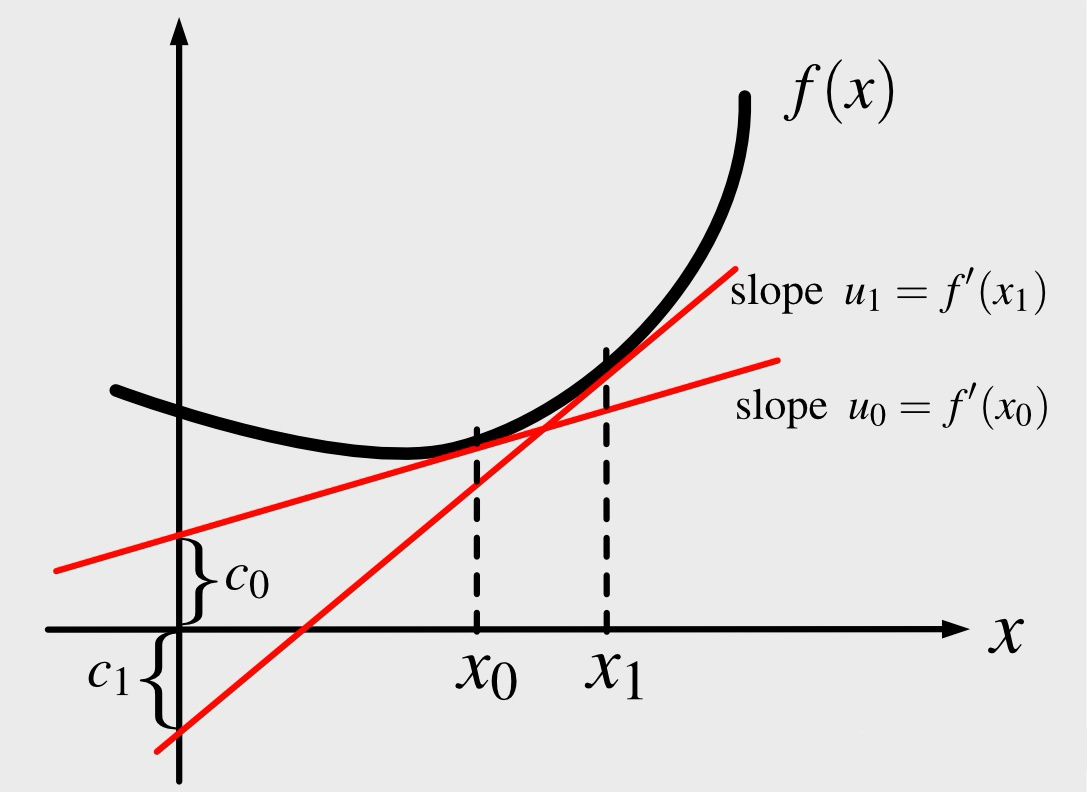
\includegraphics[scale=0.2]{./fig/Legendre Transform/1.png}
\end{figure}

一维情形下,如果我们想利用$f(x)$在某点$x_0$的切线斜率$u_0=f'(x_0)$确定$f(x_0)$,我们还需要知道这条切线的纵截距记为$c(x_0)$:
\[f(x_0)=f'(x_0)x_0+c(x_0)\]
我们也可以进一步将上式扩展到全定义域:
\[f(x)=f'(x)x+c(x)\]
由于切线斜率是已知的,所以这里我们更希望得到一个曲线斜率“表象”下的信息而非目前现有的坐标“表象”。因此,我们希望引入反函数
\[x=[f']^{-1}(u)\]
易知,这里我们要求$f':x \rightarrow u$是一个双射,故一般我们要求做$Legendre$变换的对象函数$f$是凸的,
当然也可以是凹的,不过一般物理上需要做$Legendre$变换的能量项都是凸的,故我们一般都默认$Legendre$变换是定义在凸函数上的。

明确上述要求后,我们继续往下
\[f([f']^{-1}(u))=u[f']^{-1}(u)+c([f']^{-1}(u))\]
这时,我们引入记号$\tilde{f}(u)$\textbf{称做$f(x)$的$Legendre$变换}:
\[\tilde{f}(u):=-c([f']^{-1}(u))=ux-f(x)\]

\begin{definition}[一维$Legendre$变换]
    定义$f(x)$为一个实变量的实值凸函数,我们称$\tilde{f}(u)$为$f(x)$的$Legendre$变换如果其满足
    \[\tilde{f}(u)=ux-f(x)\]
\end{definition}

函数的曲线$x \ vs. \ f(x)$表示的信息与由它在所有点的切线斜率$u=f'(x)$和截距$-\tilde{f}(u)$完全等价。
如果把图中所有点的的切线都画出来,它们描绘(切)出的曲线边缘就是$f(x)$的形状。
\begin{figure}[htbp]
    \centering
    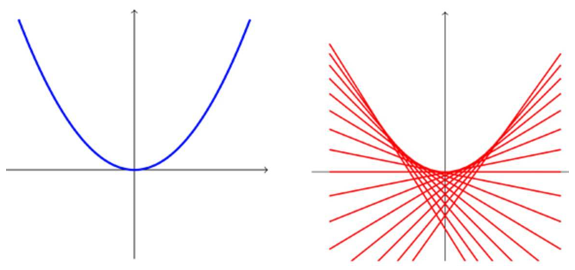
\includegraphics[scale=0.8]{./fig/Legendre Transform/2.png}
\end{figure}
所以说$Legendre$变换将点与线的信息关联起来,也称作对偶性($duality$)。
$f(x)$和$\tilde{f}(u)$互为$Legendre$变换,且$Legendre$变换具有对合性,即$\tilde{\tilde{f}}=f$。

$Legendre$变换是一个实变量的实值凸函数的对合变换,代数意义上,$Legendre$变换是一将向量空间($Vector \ space$)映射到对偶空间($Dual \ Space$)的双射;
在微分几何语言描述中它是切丛到余切丛的同构映射。

进而我们可以二维情形,给定二元凸函数$f(x,y)$,其全微分如下:
\[df=\frac{\partial f}{\partial x}dx+\frac{\partial f}{\partial y}dy:=udx+vdy\]

考虑表象变换$(x,y) \ \rightarrow \ (u,v)$:
\[\frac{\partial f}{\partial u}=\frac{\partial f}{\partial x}\frac{\partial x}{\partial u}+\frac{\partial f}{\partial y}\frac{\partial y}{\partial u}=u\frac{\partial x}{\partial u}+v\frac{\partial y}{\partial u}=\frac{\partial (ux)}{\partial u}-x+v\frac{\partial y}{\partial u}\]
\[\frac{\partial f}{\partial v}=\frac{\partial f}{\partial x}\frac{\partial x}{\partial v}+\frac{\partial f}{\partial y}\frac{\partial y}{\partial v}=u\frac{\partial x}{\partial v}+v\frac{\partial y}{\partial v}=u\frac{\partial x}{\partial v}+\frac{\partial (vy)}{\partial v}-y\]
易得
\[x=\frac{\partial (ux+vy-f)}{\partial u}:=\frac{\partial \tilde{f}}{\partial u}\]
\[y=\frac{\partial (ux+vy-f)}{\partial v}:=\frac{\partial \tilde{f}}{\partial v}\]

同样地,我们也可以定义n维$Legendre$变换。

\begin{definition}[n维$Legendre$变换]
    定义$f(x_1,x_2,\cdots,x_n)$为一个实变量的实值凸函数,我们称$\tilde{f}(u_1,u_2,\cdots,u_n)$为$f(x_1,x_2,\cdots,x_n)$的$Legendre$变换如果其满足
    \[\tilde{f}(u_1,u_2,\cdots,u_n)=\sum_{i=1}^nx_iu_i-f(x_1,x_2,\cdots,x_n)\]
    其中
    \[u_i=\frac{\partial f}{\partial x} \qquad x_i=\frac{\partial \tilde{f}}{\partial u} \qquad (i-1,2,\cdots,n)\]
\end{definition}

容易验证
\[d\tilde{f}=\sum_{i=1}^n(x_idu_i+u_idx_i)-df=\sum_{i=1}^nx_idu_i \qquad x_i=\frac{\partial \tilde{f}}{\partial u} \qquad (i-1,2,\cdots,n)\]

$Legendre$变换在热力学上有应用,其中一个例子就是四个热力学函数之间的转换,四个热力学函数的相互转化关系如下
\[U=U(S,V)\]
\[H=H(S,p)=U+pV \qquad F=F(T,V)=U-TS \qquad G=G(T,p)=H-TS=U+pV-TS\]
由
\[dU=TdS-pdV\]
可以得到其他函数的全微分
\[dH=d(U+pV)=TdS-pdV+pdV+Vdp=TdS+Vdp=dH(S,p)\]
\[dF=d(U-TS)=TdS-pdV-TdS-SdT=-SdT-pdV=dF(T,V)\]
\[dG=d(U+pV-TS)=TdS-pdV+pdV+Vdp-TdS-SdT=Vdp-SdT=dG(T,p)\]

进而可以得到$Maxwell$关系
\[dU=TdS-pdV \quad \Rightarrow \quad \left(\frac{\partial T}{\partial V}\right)_S=-\left(\frac{\partial p}{\partial S}\right)_V\]
\[dH=TdS+Vdp \quad \Rightarrow \quad \left(\frac{\partial T}{\partial p}\right)_S=\left(\frac{\partial V}{\partial S}\right)_p\]
\[dF=-SdT-pdV \quad \Rightarrow \quad \left(\frac{\partial S}{\partial V}\right)_T=\left(\frac{\partial p}{\partial T}\right)_V\]
\[dG=Vdp-SdT \quad \Rightarrow \quad \left(\frac{\partial S}{\partial p}\right)_T=-\left(\frac{\partial V}{\partial T}\right)_p\]

在经典力学中,拉格朗日量到哈密顿量的变换也是有$Legendre$变换完成的。
$Lagrangian$可以描述为$L=L(\mathbf{q},\dot{\mathbf{q}},t)$这里$q_i$、$\dot{q}_i$、$t$分别为广义坐标、广义速度和一维时间。利用$Euler-Lagrange$方程
\[\frac{d}{dt}\frac{\partial L}{\partial \dot{q}_i}=\frac{\partial L}{\partial q_i}\]
对$L$求全微分
\[dL=\sum_i\frac{\partial L}{\partial q_i}dq_i+\sum_i\frac{\partial L}{\partial \dot{q}_i}d\dot{q}_i+\frac{\partial L}{\partial t}dt
=\sum_i\frac{\partial L}{\partial q_i}dq_i+\sum_i\left[d\left(\frac{\partial L}{\partial \dot{q}_i}\dot{q}_i\right)-\dot{q}_id\left(\frac{\partial L}{\partial \dot{q}_i}\right)\right]+\frac{\partial L}{\partial t}dt\]

现引入广义动量$p_i$
\[\dot{p_i}=\frac{d}{dt}\frac{\partial L}{\partial \dot{q}_i}=\frac{\partial L}{\partial q_i}\]
则
\[dL=\sum_i\dot{p_i}dq_i+\sum_id\left(p_i\dot{q}_i\right)-\sum_i\dot{q}_idp_i+\frac{\partial L}{\partial t}dt\]
$Hamiltonian$是广义坐标、广义动量和时间的函数$H=H(\mathbf{q},\mathbf{p},t)$,利用$Legendre$变换
\[H(\mathbf{q},\mathbf{p},t)=\sum_ip_i\dot{q}_i-L(\mathbf{q},\dot{\mathbf{q}},t)\]
\[dH=\sum_id\left(p_i\dot{q}_i\right)-dL=\sum_i\dot{q}_idp_i-\sum_i\dot{p_i}dq_i-\frac{\partial L}{\partial t}dt\]

直接对$H$求全微分
\[dH=\sum_i\frac{\partial H}{\partial q_i}dq_i+\sum_i\frac{\partial H}{\partial p_i}dp_i+\frac{\partial H}{\partial t}dt\]
可得\textbf{$Hamilton$正则运动方程}
\[\dot{q}_i=\frac{\partial H}{\partial p_i} \qquad \dot{p}_i=-\frac{\partial H}{\partial q_i} \qquad (i=1,2,\cdots,n)\]
以及
\[\frac{\partial L}{\partial t}=-\frac{\partial H}{\partial t}\]
\textbf{注意:拉格朗日力学里广义坐标和广义速度是相互独立的,哈密顿力学里广义坐标和广义动量是相互独立的!}

\section{绝热表象和透热表象}
\chapter{讨论题}
\section{如何理解原子、分子上电子运动范围和能量的关系}
运动范围可以考虑成以下两种情况,一是最概然分布位置,二是边界束缚。

首先考虑最概然分布位置,最概然分布的情况对应于波函数的收敛性质不依赖于边界条件,如氢原子中的轨道等,在这种情况下主量子数决定了轨道的最概然分布位置$<r>$,主量子数越大,$<r>$越大,$<V>$势能越大,考虑位力定理,$2<T>=n<V>$,这里取$n=-1$,体系能量的均值$<E>=-\frac{1}{2}<V>$越大。

其次考虑边界束缚,边界束缚的条件对应于波函数收敛性质与边界条件有关,如势箱,在这种情况下,电子的运动范围越广,能量越低。

\end{document}
